\documentclass[twoside]{book}

% Packages required by doxygen
\usepackage{fixltx2e}
\usepackage{calc}
\usepackage{doxygen}
\usepackage[export]{adjustbox} % also loads graphicx
\usepackage{graphicx}
\usepackage[utf8]{inputenc}
\usepackage{makeidx}
\usepackage{multicol}
\usepackage{multirow}
\PassOptionsToPackage{warn}{textcomp}
\usepackage{textcomp}
\usepackage[nointegrals]{wasysym}
\usepackage[table]{xcolor}

% Font selection
\usepackage[T1]{fontenc}
\usepackage[scaled=.90]{helvet}
\usepackage{courier}
\usepackage{amssymb}
\usepackage{sectsty}
\renewcommand{\familydefault}{\sfdefault}
\allsectionsfont{%
  \fontseries{bc}\selectfont%
  \color{darkgray}%
}
\renewcommand{\DoxyLabelFont}{%
  \fontseries{bc}\selectfont%
  \color{darkgray}%
}
\newcommand{\+}{\discretionary{\mbox{\scriptsize$\hookleftarrow$}}{}{}}

% Page & text layout
\usepackage{geometry}
\geometry{%
  a4paper,%
  top=2.5cm,%
  bottom=2.5cm,%
  left=2.5cm,%
  right=2.5cm%
}
\tolerance=750
\hfuzz=15pt
\hbadness=750
\setlength{\emergencystretch}{15pt}
\setlength{\parindent}{0cm}
\setlength{\parskip}{3ex plus 2ex minus 2ex}
\makeatletter
\renewcommand{\paragraph}{%
  \@startsection{paragraph}{4}{0ex}{-1.0ex}{1.0ex}{%
    \normalfont\normalsize\bfseries\SS@parafont%
  }%
}
\renewcommand{\subparagraph}{%
  \@startsection{subparagraph}{5}{0ex}{-1.0ex}{1.0ex}{%
    \normalfont\normalsize\bfseries\SS@subparafont%
  }%
}
\makeatother

% Headers & footers
\usepackage{fancyhdr}
\pagestyle{fancyplain}
\fancyhead[LE]{\fancyplain{}{\bfseries\thepage}}
\fancyhead[CE]{\fancyplain{}{}}
\fancyhead[RE]{\fancyplain{}{\bfseries\leftmark}}
\fancyhead[LO]{\fancyplain{}{\bfseries\rightmark}}
\fancyhead[CO]{\fancyplain{}{}}
\fancyhead[RO]{\fancyplain{}{\bfseries\thepage}}
\fancyfoot[LE]{\fancyplain{}{}}
\fancyfoot[CE]{\fancyplain{}{}}
\fancyfoot[RE]{\fancyplain{}{\bfseries\scriptsize Generated by Doxygen }}
\fancyfoot[LO]{\fancyplain{}{\bfseries\scriptsize Generated by Doxygen }}
\fancyfoot[CO]{\fancyplain{}{}}
\fancyfoot[RO]{\fancyplain{}{}}
\renewcommand{\footrulewidth}{0.4pt}
\renewcommand{\chaptermark}[1]{%
  \markboth{#1}{}%
}
\renewcommand{\sectionmark}[1]{%
  \markright{\thesection\ #1}%
}

% Indices & bibliography
\usepackage{natbib}
\usepackage[titles]{tocloft}
\setcounter{tocdepth}{3}
\setcounter{secnumdepth}{5}
\makeindex

% Hyperlinks (required, but should be loaded last)
\usepackage{ifpdf}
\ifpdf
  \usepackage[pdftex,pagebackref=true]{hyperref}
\else
  \usepackage[ps2pdf,pagebackref=true]{hyperref}
\fi
\hypersetup{%
  colorlinks=true,%
  linkcolor=blue,%
  citecolor=blue,%
  unicode%
}

% Custom commands
\newcommand{\clearemptydoublepage}{%
  \newpage{\pagestyle{empty}\cleardoublepage}%
}

\usepackage{caption}
\captionsetup{labelsep=space,justification=centering,font={bf},singlelinecheck=off,skip=4pt,position=top}

%===== C O N T E N T S =====

\begin{document}

% Titlepage & ToC
\hypersetup{pageanchor=false,
             bookmarksnumbered=true,
             pdfencoding=unicode
            }
\pagenumbering{alph}
\begin{titlepage}
\vspace*{7cm}
\begin{center}%
{\Large Application\+Documentation }\\
\vspace*{1cm}
{\large Generated by Doxygen 1.8.14}\\
\end{center}
\end{titlepage}
\clearemptydoublepage
\pagenumbering{roman}
\tableofcontents
\clearemptydoublepage
\pagenumbering{arabic}
\hypersetup{pageanchor=true}

%--- Begin generated contents ---
\chapter{Namespace Index}
\section{Packages}
Here are the packages with brief descriptions (if available)\+:\begin{DoxyCompactList}
\item\contentsline{section}{\mbox{\hyperlink{namespace_application}{Application}} }{\pageref{namespace_application}}{}
\item\contentsline{section}{\mbox{\hyperlink{namespace_application_1_1_controllers}{Application.\+Controllers}} }{\pageref{namespace_application_1_1_controllers}}{}
\item\contentsline{section}{\mbox{\hyperlink{namespace_application_1_1_interfaces}{Application.\+Interfaces}} }{\pageref{namespace_application_1_1_interfaces}}{}
\item\contentsline{section}{\mbox{\hyperlink{namespace_application_1_1_managers}{Application.\+Managers}} }{\pageref{namespace_application_1_1_managers}}{}
\item\contentsline{section}{\mbox{\hyperlink{namespace_application_1_1_misc}{Application.\+Misc}} }{\pageref{namespace_application_1_1_misc}}{}
\end{DoxyCompactList}

\chapter{Hierarchical Index}
\section{Class Hierarchy}
This inheritance list is sorted roughly, but not completely, alphabetically\+:\begin{DoxyCompactList}
\item \contentsline{section}{Application.\+Misc.\+Cache\+List$<$ T\+Class $>$}{\pageref{class_application_1_1_misc_1_1_cache_list}}{}
\item \contentsline{section}{Application.\+Misc.\+Cache\+List$<$ string $>$}{\pageref{class_application_1_1_misc_1_1_cache_list}}{}
\item \contentsline{section}{Application.\+Misc.\+Cache\+List$<$ T\+Class $>$.Contained\+Item}{\pageref{class_application_1_1_misc_1_1_cache_list_1_1_contained_item}}{}
\item Event\+Args\begin{DoxyCompactList}
\item \contentsline{section}{Application.\+Interfaces.\+Timed\+Out\+User\+Event\+Args}{\pageref{class_application_1_1_interfaces_1_1_timed_out_user_event_args}}{}
\end{DoxyCompactList}
\item \contentsline{section}{Application.\+Misc.\+I\+Cache\+Handle}{\pageref{interface_application_1_1_misc_1_1_i_cache_handle}}{}
\item I\+Disposable\begin{DoxyCompactList}
\item \contentsline{section}{Application.\+Misc.\+Smart\+Lock.\+Releaser}{\pageref{struct_application_1_1_misc_1_1_smart_lock_1_1_releaser}}{}
\end{DoxyCompactList}
\item \contentsline{section}{Application.\+Interfaces.\+I\+Game\+Controller}{\pageref{interface_application_1_1_interfaces_1_1_i_game_controller}}{}
\begin{DoxyCompactList}
\item \contentsline{section}{Application.\+Controllers.\+Game\+Controller}{\pageref{class_application_1_1_controllers_1_1_game_controller}}{}
\end{DoxyCompactList}
\item \contentsline{section}{Application.\+Interfaces.\+I\+Lobby\+Controller}{\pageref{interface_application_1_1_interfaces_1_1_i_lobby_controller}}{}
\begin{DoxyCompactList}
\item \contentsline{section}{Application.\+Controllers.\+Lobby\+Controller}{\pageref{class_application_1_1_controllers_1_1_lobby_controller}}{}
\end{DoxyCompactList}
\item \contentsline{section}{Application.\+Interfaces.\+I\+Lobby\+Pool}{\pageref{interface_application_1_1_interfaces_1_1_i_lobby_pool}}{}
\begin{DoxyCompactList}
\item \contentsline{section}{Application.\+Misc.\+Lobby\+Pool}{\pageref{class_application_1_1_misc_1_1_lobby_pool}}{}
\end{DoxyCompactList}
\item \contentsline{section}{Application.\+Interfaces.\+I\+Login\+Manager}{\pageref{interface_application_1_1_interfaces_1_1_i_login_manager}}{}
\begin{DoxyCompactList}
\item \contentsline{section}{Application.\+Managers.\+Login\+Manager}{\pageref{class_application_1_1_managers_1_1_login_manager}}{}
\end{DoxyCompactList}
\item \contentsline{section}{Application.\+Interfaces.\+I\+Timer}{\pageref{interface_application_1_1_interfaces_1_1_i_timer}}{}
\begin{DoxyCompactList}
\item \contentsline{section}{Application.\+Misc.\+Count\+Down\+Timer}{\pageref{class_application_1_1_misc_1_1_count_down_timer}}{}
\end{DoxyCompactList}
\item \contentsline{section}{Application.\+Interfaces.\+I\+User\+Cache}{\pageref{interface_application_1_1_interfaces_1_1_i_user_cache}}{}
\begin{DoxyCompactList}
\item \contentsline{section}{Application.\+Misc.\+User\+Cache}{\pageref{class_application_1_1_misc_1_1_user_cache}}{}
\end{DoxyCompactList}
\item \contentsline{section}{Application.\+Interfaces.\+I\+User\+Controller}{\pageref{interface_application_1_1_interfaces_1_1_i_user_controller}}{}
\begin{DoxyCompactList}
\item \contentsline{section}{Application.\+Controllers.\+User\+Controller}{\pageref{class_application_1_1_controllers_1_1_user_controller}}{}
\end{DoxyCompactList}
\item \contentsline{section}{Application.\+Misc.\+Smart\+Lock}{\pageref{class_application_1_1_misc_1_1_smart_lock}}{}
\end{DoxyCompactList}

\chapter{Class Index}
\section{Class List}
Here are the classes, structs, unions and interfaces with brief descriptions\+:\begin{DoxyCompactList}
\item\contentsline{section}{\mbox{\hyperlink{class_application_1_1_misc_1_1_cache_list}{Application.\+Misc.\+Cache\+List$<$ T\+Class $>$}} }{\pageref{class_application_1_1_misc_1_1_cache_list}}{}
\item\contentsline{section}{\mbox{\hyperlink{class_application_1_1_misc_1_1_cache_list_1_1_contained_item}{Application.\+Misc.\+Cache\+List$<$ T\+Class $>$.\+Contained\+Item}} }{\pageref{class_application_1_1_misc_1_1_cache_list_1_1_contained_item}}{}
\item\contentsline{section}{\mbox{\hyperlink{class_application_1_1_misc_1_1_count_down_timer}{Application.\+Misc.\+Count\+Down\+Timer}} }{\pageref{class_application_1_1_misc_1_1_count_down_timer}}{}
\item\contentsline{section}{\mbox{\hyperlink{class_application_1_1_controllers_1_1_game_controller}{Application.\+Controllers.\+Game\+Controller}} }{\pageref{class_application_1_1_controllers_1_1_game_controller}}{}
\item\contentsline{section}{\mbox{\hyperlink{interface_application_1_1_misc_1_1_i_cache_handle}{Application.\+Misc.\+I\+Cache\+Handle}} }{\pageref{interface_application_1_1_misc_1_1_i_cache_handle}}{}
\item\contentsline{section}{\mbox{\hyperlink{interface_application_1_1_interfaces_1_1_i_game_controller}{Application.\+Interfaces.\+I\+Game\+Controller}} }{\pageref{interface_application_1_1_interfaces_1_1_i_game_controller}}{}
\item\contentsline{section}{\mbox{\hyperlink{interface_application_1_1_interfaces_1_1_i_lobby_controller}{Application.\+Interfaces.\+I\+Lobby\+Controller}} }{\pageref{interface_application_1_1_interfaces_1_1_i_lobby_controller}}{}
\item\contentsline{section}{\mbox{\hyperlink{interface_application_1_1_interfaces_1_1_i_lobby_pool}{Application.\+Interfaces.\+I\+Lobby\+Pool}} }{\pageref{interface_application_1_1_interfaces_1_1_i_lobby_pool}}{}
\item\contentsline{section}{\mbox{\hyperlink{interface_application_1_1_interfaces_1_1_i_login_manager}{Application.\+Interfaces.\+I\+Login\+Manager}} }{\pageref{interface_application_1_1_interfaces_1_1_i_login_manager}}{}
\item\contentsline{section}{\mbox{\hyperlink{interface_application_1_1_interfaces_1_1_i_timer}{Application.\+Interfaces.\+I\+Timer}} }{\pageref{interface_application_1_1_interfaces_1_1_i_timer}}{}
\item\contentsline{section}{\mbox{\hyperlink{interface_application_1_1_interfaces_1_1_i_user_cache}{Application.\+Interfaces.\+I\+User\+Cache}} }{\pageref{interface_application_1_1_interfaces_1_1_i_user_cache}}{}
\item\contentsline{section}{\mbox{\hyperlink{interface_application_1_1_interfaces_1_1_i_user_controller}{Application.\+Interfaces.\+I\+User\+Controller}} }{\pageref{interface_application_1_1_interfaces_1_1_i_user_controller}}{}
\item\contentsline{section}{\mbox{\hyperlink{class_application_1_1_controllers_1_1_lobby_controller}{Application.\+Controllers.\+Lobby\+Controller}} }{\pageref{class_application_1_1_controllers_1_1_lobby_controller}}{}
\item\contentsline{section}{\mbox{\hyperlink{class_application_1_1_misc_1_1_lobby_pool}{Application.\+Misc.\+Lobby\+Pool}} }{\pageref{class_application_1_1_misc_1_1_lobby_pool}}{}
\item\contentsline{section}{\mbox{\hyperlink{class_application_1_1_managers_1_1_login_manager}{Application.\+Managers.\+Login\+Manager}} }{\pageref{class_application_1_1_managers_1_1_login_manager}}{}
\item\contentsline{section}{\mbox{\hyperlink{struct_application_1_1_misc_1_1_smart_lock_1_1_releaser}{Application.\+Misc.\+Smart\+Lock.\+Releaser}} }{\pageref{struct_application_1_1_misc_1_1_smart_lock_1_1_releaser}}{}
\item\contentsline{section}{\mbox{\hyperlink{class_application_1_1_misc_1_1_smart_lock}{Application.\+Misc.\+Smart\+Lock}} \\*Inspired by\+: \href{https://blogs.msdn.microsoft.com/pfxteam/2012/02/12/building-async-coordination-primitives-part-6-asynclock/}{\tt https\+://blogs.\+msdn.\+microsoft.\+com/pfxteam/2012/02/12/building-\/async-\/coordination-\/primitives-\/part-\/6-\/asynclock/} }{\pageref{class_application_1_1_misc_1_1_smart_lock}}{}
\item\contentsline{section}{\mbox{\hyperlink{class_application_1_1_interfaces_1_1_timed_out_user_event_args}{Application.\+Interfaces.\+Timed\+Out\+User\+Event\+Args}} }{\pageref{class_application_1_1_interfaces_1_1_timed_out_user_event_args}}{}
\item\contentsline{section}{\mbox{\hyperlink{class_application_1_1_misc_1_1_user_cache}{Application.\+Misc.\+User\+Cache}} }{\pageref{class_application_1_1_misc_1_1_user_cache}}{}
\item\contentsline{section}{\mbox{\hyperlink{class_application_1_1_controllers_1_1_user_controller}{Application.\+Controllers.\+User\+Controller}} \\*\mbox{\hyperlink{namespace_application}{Application}} User Controller The main purpose of this class is to decouple the framework from our application logic }{\pageref{class_application_1_1_controllers_1_1_user_controller}}{}
\end{DoxyCompactList}

\chapter{File Index}
\section{File List}
Here is a list of all files with brief descriptions\+:\begin{DoxyCompactList}
\item\contentsline{section}{\mbox{\hyperlink{_program_8cs}{Program.\+cs}} }{\pageref{_program_8cs}}{}
\item\contentsline{section}{\mbox{\hyperlink{_startup_8cs}{Startup.\+cs}} }{\pageref{_startup_8cs}}{}
\item\contentsline{section}{Filters/\mbox{\hyperlink{_authorization_swag_attribute_8cs}{Authorization\+Swag\+Attribute.\+cs}} }{\pageref{_authorization_swag_attribute_8cs}}{}
\item\contentsline{section}{Filters/\mbox{\hyperlink{_require_from_query_attribute_8cs}{Require\+From\+Query\+Attribute.\+cs}} }{\pageref{_require_from_query_attribute_8cs}}{}
\item\contentsline{section}{Filters/\mbox{\hyperlink{_validate_model_state_attribute_8cs}{Validate\+Model\+State\+Attribute.\+cs}} }{\pageref{_validate_model_state_attribute_8cs}}{}
\item\contentsline{section}{Formatters/\mbox{\hyperlink{_json_input_formatter_8cs}{Json\+Input\+Formatter.\+cs}} }{\pageref{_json_input_formatter_8cs}}{}
\item\contentsline{section}{Interfaces/\mbox{\hyperlink{_i_lobby_controller_8cs}{I\+Lobby\+Controller.\+cs}} }{\pageref{_i_lobby_controller_8cs}}{}
\item\contentsline{section}{Json\+Serializer\+Extensions/\mbox{\hyperlink{_utility_8cs}{Utility.\+cs}} }{\pageref{_utility_8cs}}{}
\item\contentsline{section}{Model\+Binders(\+Deprecated)/\mbox{\hyperlink{_from_swag_dto_model_binder_8cs}{From\+Swag\+Dto\+Model\+Binder.\+cs}} }{\pageref{_from_swag_dto_model_binder_8cs}}{}
\item\contentsline{section}{Model\+Binders(\+Deprecated)/\+Attributes/\mbox{\hyperlink{_from_swag_dto_attribute_8cs}{From\+Swag\+Dto\+Attribute.\+cs}} }{\pageref{_from_swag_dto_attribute_8cs}}{}
\item\contentsline{section}{Model\+Binders(\+Deprecated)/\+Attributes/\mbox{\hyperlink{_i_from_swag_dto_attribute_8cs}{I\+From\+Swag\+Dto\+Attribute.\+cs}} }{\pageref{_i_from_swag_dto_attribute_8cs}}{}
\item\contentsline{section}{Model\+Binders(\+Deprecated)/\+Value\+Providers/\mbox{\hyperlink{_from_dto_value_provider_8cs}{From\+Dto\+Value\+Provider.\+cs}} }{\pageref{_from_dto_value_provider_8cs}}{}
\item\contentsline{section}{Model\+Binders(\+Deprecated)/\+Value\+Providers/\mbox{\hyperlink{_from_dto_value_provider_factory_8cs}{From\+Dto\+Value\+Provider\+Factory.\+cs}} }{\pageref{_from_dto_value_provider_factory_8cs}}{}
\item\contentsline{section}{obj/\+Debug/netcoreapp2.\+0/\mbox{\hyperlink{_debug_2netcoreapp2_80_2_communication_8_assembly_info_8cs}{Communication.\+Assembly\+Info.\+cs}} }{\pageref{_debug_2netcoreapp2_80_2_communication_8_assembly_info_8cs}}{}
\item\contentsline{section}{obj/\+Release/netcoreapp2.\+0/\mbox{\hyperlink{_release_2netcoreapp2_80_2_communication_8_assembly_info_8cs}{Communication.\+Assembly\+Info.\+cs}} }{\pageref{_release_2netcoreapp2_80_2_communication_8_assembly_info_8cs}}{}
\item\contentsline{section}{R\+E\+S\+T\+Controllers/\mbox{\hyperlink{_lobby_controller_8cs}{Lobby\+Controller.\+cs}} }{\pageref{_lobby_controller_8cs}}{}
\item\contentsline{section}{R\+E\+S\+T\+Controllers/\mbox{\hyperlink{_user_controller_8cs}{User\+Controller.\+cs}} }{\pageref{_user_controller_8cs}}{}
\end{DoxyCompactList}

\chapter{Namespace Documentation}
\hypertarget{namespace_application}{}\section{Application Namespace Reference}
\label{namespace_application}\index{Application@{Application}}
\subsection*{Namespaces}
\begin{DoxyCompactItemize}
\item 
namespace \mbox{\hyperlink{namespace_application_1_1_controllers}{Controllers}}
\item 
namespace \mbox{\hyperlink{namespace_application_1_1_interfaces}{Interfaces}}
\item 
namespace \mbox{\hyperlink{namespace_application_1_1_managers}{Managers}}
\item 
namespace \mbox{\hyperlink{namespace_application_1_1_misc}{Misc}}
\end{DoxyCompactItemize}

\hypertarget{namespace_application_1_1_controllers}{}\section{Application.\+Controllers Namespace Reference}
\label{namespace_application_1_1_controllers}\index{Application.\+Controllers@{Application.\+Controllers}}
\subsection*{Classes}
\begin{DoxyCompactItemize}
\item 
class \mbox{\hyperlink{class_application_1_1_controllers_1_1_game_controller}{Game\+Controller}}
\item 
class \mbox{\hyperlink{class_application_1_1_controllers_1_1_lobby_controller}{Lobby\+Controller}}
\item 
class \mbox{\hyperlink{class_application_1_1_controllers_1_1_user_controller}{User\+Controller}}
\begin{DoxyCompactList}\small\item\em \mbox{\hyperlink{namespace_application}{Application}} User Controller The main purpose of this class is to decouple the framework from our application logic \end{DoxyCompactList}\end{DoxyCompactItemize}

\hypertarget{namespace_application_1_1_interfaces}{}\section{Application.\+Interfaces Namespace Reference}
\label{namespace_application_1_1_interfaces}\index{Application.\+Interfaces@{Application.\+Interfaces}}
\subsection*{Classes}
\begin{DoxyCompactItemize}
\item 
interface \mbox{\hyperlink{interface_application_1_1_interfaces_1_1_i_game_controller}{I\+Game\+Controller}}
\item 
interface \mbox{\hyperlink{interface_application_1_1_interfaces_1_1_i_lobby_controller}{I\+Lobby\+Controller}}
\item 
interface \mbox{\hyperlink{interface_application_1_1_interfaces_1_1_i_lobby_pool}{I\+Lobby\+Pool}}
\item 
interface \mbox{\hyperlink{interface_application_1_1_interfaces_1_1_i_login_manager}{I\+Login\+Manager}}
\item 
interface \mbox{\hyperlink{interface_application_1_1_interfaces_1_1_i_timer}{I\+Timer}}
\item 
interface \mbox{\hyperlink{interface_application_1_1_interfaces_1_1_i_user_cache}{I\+User\+Cache}}
\item 
interface \mbox{\hyperlink{interface_application_1_1_interfaces_1_1_i_user_controller}{I\+User\+Controller}}
\item 
class \mbox{\hyperlink{class_application_1_1_interfaces_1_1_timed_out_user_event_args}{Timed\+Out\+User\+Event\+Args}}
\end{DoxyCompactItemize}
\subsection*{Functions}
\begin{DoxyCompactItemize}
\item 
delegate void \mbox{\hyperlink{namespace_application_1_1_interfaces_a3ba96a057acca29f3e2e533aeb2f30e0}{User\+Logged\+Out\+Handle}} (object obj, string username)
\begin{DoxyCompactList}\small\item\em The handler for \textquotesingle{}User Logged-\/\+Out\textquotesingle{} events \end{DoxyCompactList}\end{DoxyCompactItemize}


\subsection{Function Documentation}
\mbox{\Hypertarget{namespace_application_1_1_interfaces_a3ba96a057acca29f3e2e533aeb2f30e0}\label{namespace_application_1_1_interfaces_a3ba96a057acca29f3e2e533aeb2f30e0}} 
\index{Application\+::\+Interfaces@{Application\+::\+Interfaces}!User\+Logged\+Out\+Handle@{User\+Logged\+Out\+Handle}}
\index{User\+Logged\+Out\+Handle@{User\+Logged\+Out\+Handle}!Application\+::\+Interfaces@{Application\+::\+Interfaces}}
\subsubsection{\texorpdfstring{User\+Logged\+Out\+Handle()}{UserLoggedOutHandle()}}
{\footnotesize\ttfamily delegate void Application.\+Interfaces.\+User\+Logged\+Out\+Handle (\begin{DoxyParamCaption}\item[{object}]{obj,  }\item[{string}]{username }\end{DoxyParamCaption})}



The handler for \textquotesingle{}User Logged-\/\+Out\textquotesingle{} events 


\begin{DoxyParams}{Parameters}
{\em obj} & \\
\hline
{\em username} & \\
\hline
\end{DoxyParams}

\hypertarget{namespace_application_1_1_managers}{}\section{Application.\+Managers Namespace Reference}
\label{namespace_application_1_1_managers}\index{Application.\+Managers@{Application.\+Managers}}
\subsection*{Classes}
\begin{DoxyCompactItemize}
\item 
class \mbox{\hyperlink{class_application_1_1_managers_1_1_login_manager}{Login\+Manager}}
\end{DoxyCompactItemize}

\hypertarget{namespace_application_1_1_misc}{}\section{Application.\+Misc Namespace Reference}
\label{namespace_application_1_1_misc}\index{Application.\+Misc@{Application.\+Misc}}
\subsection*{Classes}
\begin{DoxyCompactItemize}
\item 
class \mbox{\hyperlink{class_application_1_1_misc_1_1_cache_list}{Cache\+List}}
\item 
class \mbox{\hyperlink{class_application_1_1_misc_1_1_count_down_timer}{Count\+Down\+Timer}}
\item 
class {\bfseries Date\+Time\+Extentions}
\item 
class {\bfseries Date\+Time\+Helper}
\item 
interface \mbox{\hyperlink{interface_application_1_1_misc_1_1_i_cache_handle}{I\+Cache\+Handle}}
\item 
class \mbox{\hyperlink{class_application_1_1_misc_1_1_lobby_pool}{Lobby\+Pool}}
\item 
class \mbox{\hyperlink{class_application_1_1_misc_1_1_smart_lock}{Smart\+Lock}}
\begin{DoxyCompactList}\small\item\em Inspired by\+: \href{https://blogs.msdn.microsoft.com/pfxteam/2012/02/12/building-async-coordination-primitives-part-6-asynclock/}{\tt https\+://blogs.\+msdn.\+microsoft.\+com/pfxteam/2012/02/12/building-\/async-\/coordination-\/primitives-\/part-\/6-\/asynclock/} \end{DoxyCompactList}\item 
class \mbox{\hyperlink{class_application_1_1_misc_1_1_user_cache}{User\+Cache}}
\end{DoxyCompactItemize}

\chapter{Class Documentation}
\hypertarget{class_application_1_1_misc_1_1_cache_list}{}\section{Application.\+Misc.\+Cache\+List$<$ T\+Class $>$ Class Template Reference}
\label{class_application_1_1_misc_1_1_cache_list}\index{Application.\+Misc.\+Cache\+List$<$ T\+Class $>$@{Application.\+Misc.\+Cache\+List$<$ T\+Class $>$}}
\subsection*{Classes}
\begin{DoxyCompactItemize}
\item 
class \mbox{\hyperlink{class_application_1_1_misc_1_1_cache_list_1_1_contained_item}{Contained\+Item}}
\end{DoxyCompactItemize}
\subsection*{Public Member Functions}
\begin{DoxyCompactItemize}
\item 
\mbox{\hyperlink{class_application_1_1_misc_1_1_cache_list_aa90b33801fe1b0cba3437908aa470f25}{Cache\+List}} ()
\item 
void \mbox{\hyperlink{class_application_1_1_misc_1_1_cache_list_a00141bfa7925e94f1eb396cc00c2d9c1}{Add}} (T\+Class item, Date\+Time expiration, out \mbox{\hyperlink{interface_application_1_1_misc_1_1_i_cache_handle}{I\+Cache\+Handle}} handle)
\item 
void \mbox{\hyperlink{class_application_1_1_misc_1_1_cache_list_aa497244166710a24aa1aed9efc739256}{Remove}} (\mbox{\hyperlink{interface_application_1_1_misc_1_1_i_cache_handle}{I\+Cache\+Handle}} cache\+Handle)
\item 
void \mbox{\hyperlink{class_application_1_1_misc_1_1_cache_list_a7ffcd0d1d2df50cf6e58ad68eaeb670d}{Update}} (\mbox{\hyperlink{interface_application_1_1_misc_1_1_i_cache_handle}{I\+Cache\+Handle}} cache\+Handle, Date\+Time expiration, T\+Class item=null)
\item 
bool \mbox{\hyperlink{class_application_1_1_misc_1_1_cache_list_ab84c82298def7a9d3c11d3c401f43b45}{Contains\+Outdated\+Item}} (Date\+Time compare\+To)
\item 
T\+Class \mbox{\hyperlink{class_application_1_1_misc_1_1_cache_list_af1093c1339d895ab16286b7834d0f1c1}{Remove\+And\+Get}} ()
\end{DoxyCompactItemize}
\subsection*{Public Attributes}
\begin{DoxyCompactItemize}
\item 
I\+Read\+Only\+List$<$ \mbox{\hyperlink{class_application_1_1_misc_1_1_cache_list_1_1_contained_item}{Contained\+Item}} $>$ \mbox{\hyperlink{class_application_1_1_misc_1_1_cache_list_a76ecbd816361d086f756cbe086b505e6}{Collection}} =$>$ \+\_\+collection.\+To\+List()
\end{DoxyCompactItemize}


\subsection{Constructor \& Destructor Documentation}
\mbox{\Hypertarget{class_application_1_1_misc_1_1_cache_list_aa90b33801fe1b0cba3437908aa470f25}\label{class_application_1_1_misc_1_1_cache_list_aa90b33801fe1b0cba3437908aa470f25}} 
\index{Application\+::\+Misc\+::\+Cache\+List@{Application\+::\+Misc\+::\+Cache\+List}!Cache\+List@{Cache\+List}}
\index{Cache\+List@{Cache\+List}!Application\+::\+Misc\+::\+Cache\+List@{Application\+::\+Misc\+::\+Cache\+List}}
\subsubsection{\texorpdfstring{Cache\+List()}{CacheList()}}
{\footnotesize\ttfamily \mbox{\hyperlink{class_application_1_1_misc_1_1_cache_list}{Application.\+Misc.\+Cache\+List}}$<$ T\+Class $>$.\mbox{\hyperlink{class_application_1_1_misc_1_1_cache_list}{Cache\+List}} (\begin{DoxyParamCaption}{ }\end{DoxyParamCaption})}



\subsection{Member Function Documentation}
\mbox{\Hypertarget{class_application_1_1_misc_1_1_cache_list_a00141bfa7925e94f1eb396cc00c2d9c1}\label{class_application_1_1_misc_1_1_cache_list_a00141bfa7925e94f1eb396cc00c2d9c1}} 
\index{Application\+::\+Misc\+::\+Cache\+List@{Application\+::\+Misc\+::\+Cache\+List}!Add@{Add}}
\index{Add@{Add}!Application\+::\+Misc\+::\+Cache\+List@{Application\+::\+Misc\+::\+Cache\+List}}
\subsubsection{\texorpdfstring{Add()}{Add()}}
{\footnotesize\ttfamily void \mbox{\hyperlink{class_application_1_1_misc_1_1_cache_list}{Application.\+Misc.\+Cache\+List}}$<$ T\+Class $>$.Add (\begin{DoxyParamCaption}\item[{T\+Class}]{item,  }\item[{Date\+Time}]{expiration,  }\item[{out \mbox{\hyperlink{interface_application_1_1_misc_1_1_i_cache_handle}{I\+Cache\+Handle}}}]{handle }\end{DoxyParamCaption})}

\mbox{\Hypertarget{class_application_1_1_misc_1_1_cache_list_ab84c82298def7a9d3c11d3c401f43b45}\label{class_application_1_1_misc_1_1_cache_list_ab84c82298def7a9d3c11d3c401f43b45}} 
\index{Application\+::\+Misc\+::\+Cache\+List@{Application\+::\+Misc\+::\+Cache\+List}!Contains\+Outdated\+Item@{Contains\+Outdated\+Item}}
\index{Contains\+Outdated\+Item@{Contains\+Outdated\+Item}!Application\+::\+Misc\+::\+Cache\+List@{Application\+::\+Misc\+::\+Cache\+List}}
\subsubsection{\texorpdfstring{Contains\+Outdated\+Item()}{ContainsOutdatedItem()}}
{\footnotesize\ttfamily bool \mbox{\hyperlink{class_application_1_1_misc_1_1_cache_list}{Application.\+Misc.\+Cache\+List}}$<$ T\+Class $>$.Contains\+Outdated\+Item (\begin{DoxyParamCaption}\item[{Date\+Time}]{compare\+To }\end{DoxyParamCaption})}

\mbox{\Hypertarget{class_application_1_1_misc_1_1_cache_list_aa497244166710a24aa1aed9efc739256}\label{class_application_1_1_misc_1_1_cache_list_aa497244166710a24aa1aed9efc739256}} 
\index{Application\+::\+Misc\+::\+Cache\+List@{Application\+::\+Misc\+::\+Cache\+List}!Remove@{Remove}}
\index{Remove@{Remove}!Application\+::\+Misc\+::\+Cache\+List@{Application\+::\+Misc\+::\+Cache\+List}}
\subsubsection{\texorpdfstring{Remove()}{Remove()}}
{\footnotesize\ttfamily void \mbox{\hyperlink{class_application_1_1_misc_1_1_cache_list}{Application.\+Misc.\+Cache\+List}}$<$ T\+Class $>$.Remove (\begin{DoxyParamCaption}\item[{\mbox{\hyperlink{interface_application_1_1_misc_1_1_i_cache_handle}{I\+Cache\+Handle}}}]{cache\+Handle }\end{DoxyParamCaption})}

\mbox{\Hypertarget{class_application_1_1_misc_1_1_cache_list_af1093c1339d895ab16286b7834d0f1c1}\label{class_application_1_1_misc_1_1_cache_list_af1093c1339d895ab16286b7834d0f1c1}} 
\index{Application\+::\+Misc\+::\+Cache\+List@{Application\+::\+Misc\+::\+Cache\+List}!Remove\+And\+Get@{Remove\+And\+Get}}
\index{Remove\+And\+Get@{Remove\+And\+Get}!Application\+::\+Misc\+::\+Cache\+List@{Application\+::\+Misc\+::\+Cache\+List}}
\subsubsection{\texorpdfstring{Remove\+And\+Get()}{RemoveAndGet()}}
{\footnotesize\ttfamily T\+Class \mbox{\hyperlink{class_application_1_1_misc_1_1_cache_list}{Application.\+Misc.\+Cache\+List}}$<$ T\+Class $>$.Remove\+And\+Get (\begin{DoxyParamCaption}{ }\end{DoxyParamCaption})}

\mbox{\Hypertarget{class_application_1_1_misc_1_1_cache_list_a7ffcd0d1d2df50cf6e58ad68eaeb670d}\label{class_application_1_1_misc_1_1_cache_list_a7ffcd0d1d2df50cf6e58ad68eaeb670d}} 
\index{Application\+::\+Misc\+::\+Cache\+List@{Application\+::\+Misc\+::\+Cache\+List}!Update@{Update}}
\index{Update@{Update}!Application\+::\+Misc\+::\+Cache\+List@{Application\+::\+Misc\+::\+Cache\+List}}
\subsubsection{\texorpdfstring{Update()}{Update()}}
{\footnotesize\ttfamily void \mbox{\hyperlink{class_application_1_1_misc_1_1_cache_list}{Application.\+Misc.\+Cache\+List}}$<$ T\+Class $>$.Update (\begin{DoxyParamCaption}\item[{\mbox{\hyperlink{interface_application_1_1_misc_1_1_i_cache_handle}{I\+Cache\+Handle}}}]{cache\+Handle,  }\item[{Date\+Time}]{expiration,  }\item[{T\+Class}]{item = {\ttfamily null} }\end{DoxyParamCaption})}



\subsection{Member Data Documentation}
\mbox{\Hypertarget{class_application_1_1_misc_1_1_cache_list_a76ecbd816361d086f756cbe086b505e6}\label{class_application_1_1_misc_1_1_cache_list_a76ecbd816361d086f756cbe086b505e6}} 
\index{Application\+::\+Misc\+::\+Cache\+List@{Application\+::\+Misc\+::\+Cache\+List}!Collection@{Collection}}
\index{Collection@{Collection}!Application\+::\+Misc\+::\+Cache\+List@{Application\+::\+Misc\+::\+Cache\+List}}
\subsubsection{\texorpdfstring{Collection}{Collection}}
{\footnotesize\ttfamily I\+Read\+Only\+List$<$\mbox{\hyperlink{class_application_1_1_misc_1_1_cache_list_1_1_contained_item}{Contained\+Item}}$>$ \mbox{\hyperlink{class_application_1_1_misc_1_1_cache_list}{Application.\+Misc.\+Cache\+List}}$<$ T\+Class $>$.Collection =$>$ \+\_\+collection.\+To\+List()}



The documentation for this class was generated from the following file\+:\begin{DoxyCompactItemize}
\item 
Misc/\mbox{\hyperlink{_cache_list_8cs}{Cache\+List.\+cs}}\end{DoxyCompactItemize}

\hypertarget{class_application_1_1_misc_1_1_cache_list_1_1_contained_item}{}\section{Application.\+Misc.\+Cache\+List$<$ T\+Class $>$.Contained\+Item Class Reference}
\label{class_application_1_1_misc_1_1_cache_list_1_1_contained_item}\index{Application.\+Misc.\+Cache\+List$<$ T\+Class $>$.\+Contained\+Item@{Application.\+Misc.\+Cache\+List$<$ T\+Class $>$.\+Contained\+Item}}
\subsection*{Properties}
\begin{DoxyCompactItemize}
\item 
T\+Class \mbox{\hyperlink{class_application_1_1_misc_1_1_cache_list_1_1_contained_item_a7799bd7352a769f1f7ff540d369d4743}{Item}}\hspace{0.3cm}{\ttfamily  \mbox{[}get, set\mbox{]}}
\item 
Date\+Time \mbox{\hyperlink{class_application_1_1_misc_1_1_cache_list_1_1_contained_item_a5d6865f58fd14bfcf4d9ceb6dba91b84}{Expiration}}\hspace{0.3cm}{\ttfamily  \mbox{[}get, set\mbox{]}}
\end{DoxyCompactItemize}


\subsection{Property Documentation}
\mbox{\Hypertarget{class_application_1_1_misc_1_1_cache_list_1_1_contained_item_a5d6865f58fd14bfcf4d9ceb6dba91b84}\label{class_application_1_1_misc_1_1_cache_list_1_1_contained_item_a5d6865f58fd14bfcf4d9ceb6dba91b84}} 
\index{Application\+::\+Misc\+::\+Cache\+List\+::\+Contained\+Item@{Application\+::\+Misc\+::\+Cache\+List\+::\+Contained\+Item}!Expiration@{Expiration}}
\index{Expiration@{Expiration}!Application\+::\+Misc\+::\+Cache\+List\+::\+Contained\+Item@{Application\+::\+Misc\+::\+Cache\+List\+::\+Contained\+Item}}
\subsubsection{\texorpdfstring{Expiration}{Expiration}}
{\footnotesize\ttfamily Date\+Time \mbox{\hyperlink{class_application_1_1_misc_1_1_cache_list}{Application.\+Misc.\+Cache\+List}}$<$ T\+Class $>$.Contained\+Item.\+Expiration\hspace{0.3cm}{\ttfamily [get]}, {\ttfamily [set]}}

\mbox{\Hypertarget{class_application_1_1_misc_1_1_cache_list_1_1_contained_item_a7799bd7352a769f1f7ff540d369d4743}\label{class_application_1_1_misc_1_1_cache_list_1_1_contained_item_a7799bd7352a769f1f7ff540d369d4743}} 
\index{Application\+::\+Misc\+::\+Cache\+List\+::\+Contained\+Item@{Application\+::\+Misc\+::\+Cache\+List\+::\+Contained\+Item}!Item@{Item}}
\index{Item@{Item}!Application\+::\+Misc\+::\+Cache\+List\+::\+Contained\+Item@{Application\+::\+Misc\+::\+Cache\+List\+::\+Contained\+Item}}
\subsubsection{\texorpdfstring{Item}{Item}}
{\footnotesize\ttfamily T\+Class \mbox{\hyperlink{class_application_1_1_misc_1_1_cache_list}{Application.\+Misc.\+Cache\+List}}$<$ T\+Class $>$.Contained\+Item.\+Item\hspace{0.3cm}{\ttfamily [get]}, {\ttfamily [set]}}



The documentation for this class was generated from the following file\+:\begin{DoxyCompactItemize}
\item 
Misc/\mbox{\hyperlink{_cache_list_8cs}{Cache\+List.\+cs}}\end{DoxyCompactItemize}

\hypertarget{class_application_1_1_misc_1_1_count_down_timer}{}\section{Application.\+Misc.\+Count\+Down\+Timer Class Reference}
\label{class_application_1_1_misc_1_1_count_down_timer}\index{Application.\+Misc.\+Count\+Down\+Timer@{Application.\+Misc.\+Count\+Down\+Timer}}
Inheritance diagram for Application.\+Misc.\+Count\+Down\+Timer\+:\begin{figure}[H]
\begin{center}
\leavevmode
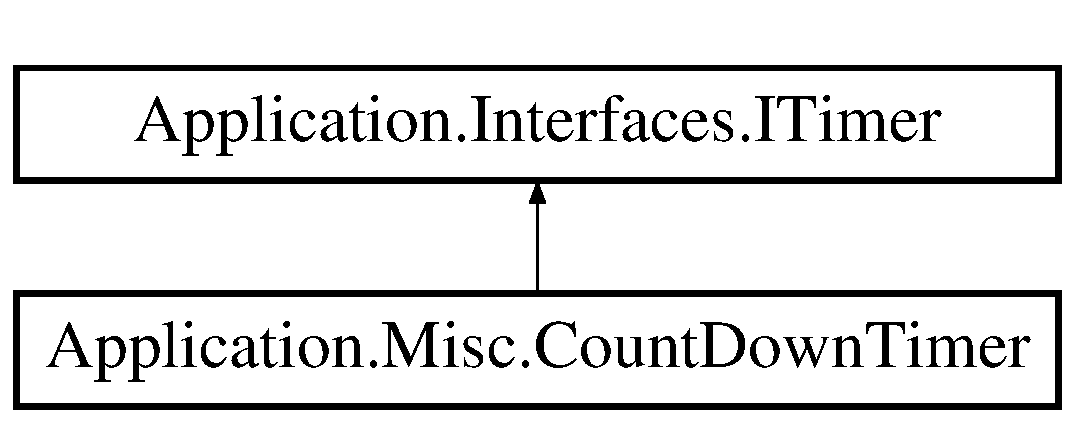
\includegraphics[height=2.000000cm]{class_application_1_1_misc_1_1_count_down_timer}
\end{center}
\end{figure}
\subsection*{Public Member Functions}
\begin{DoxyCompactItemize}
\item 
\mbox{\hyperlink{class_application_1_1_misc_1_1_count_down_timer_af178bc6b12712cd232e490c99446837d}{Count\+Down\+Timer}} ()
\item 
void \mbox{\hyperlink{class_application_1_1_misc_1_1_count_down_timer_ad07500432508a81df8f19fc55da7fc27}{Start\+With\+Seconds}} (int seconds)
\item 
void \mbox{\hyperlink{class_application_1_1_misc_1_1_count_down_timer_a46a066ed728519a096d6e47a9df080a3}{Start\+With\+Minutes}} (int minutes)
\item 
void \mbox{\hyperlink{class_application_1_1_misc_1_1_count_down_timer_a287fe196667f4c6aca7fb14506f14916}{Start}} (int minutes, int seconds)
\item 
void \mbox{\hyperlink{class_application_1_1_misc_1_1_count_down_timer_a07b90cc7a451174c7f183127d9965385}{Stop}} ()
\end{DoxyCompactItemize}
\subsection*{Events}
\begin{DoxyCompactItemize}
\item 
Event\+Handler \mbox{\hyperlink{class_application_1_1_misc_1_1_count_down_timer_a8a28f9ffa8a36fc4c71918b554fdb397}{Tick\+Event}}
\item 
Event\+Handler \mbox{\hyperlink{class_application_1_1_misc_1_1_count_down_timer_a6064d64a9bd2b1bb2ae734db384ffb46}{Expired\+Event}}
\end{DoxyCompactItemize}


\subsection{Constructor \& Destructor Documentation}
\mbox{\Hypertarget{class_application_1_1_misc_1_1_count_down_timer_af178bc6b12712cd232e490c99446837d}\label{class_application_1_1_misc_1_1_count_down_timer_af178bc6b12712cd232e490c99446837d}} 
\index{Application\+::\+Misc\+::\+Count\+Down\+Timer@{Application\+::\+Misc\+::\+Count\+Down\+Timer}!Count\+Down\+Timer@{Count\+Down\+Timer}}
\index{Count\+Down\+Timer@{Count\+Down\+Timer}!Application\+::\+Misc\+::\+Count\+Down\+Timer@{Application\+::\+Misc\+::\+Count\+Down\+Timer}}
\subsubsection{\texorpdfstring{Count\+Down\+Timer()}{CountDownTimer()}}
{\footnotesize\ttfamily Application.\+Misc.\+Count\+Down\+Timer.\+Count\+Down\+Timer (\begin{DoxyParamCaption}{ }\end{DoxyParamCaption})}



\subsection{Member Function Documentation}
\mbox{\Hypertarget{class_application_1_1_misc_1_1_count_down_timer_a287fe196667f4c6aca7fb14506f14916}\label{class_application_1_1_misc_1_1_count_down_timer_a287fe196667f4c6aca7fb14506f14916}} 
\index{Application\+::\+Misc\+::\+Count\+Down\+Timer@{Application\+::\+Misc\+::\+Count\+Down\+Timer}!Start@{Start}}
\index{Start@{Start}!Application\+::\+Misc\+::\+Count\+Down\+Timer@{Application\+::\+Misc\+::\+Count\+Down\+Timer}}
\subsubsection{\texorpdfstring{Start()}{Start()}}
{\footnotesize\ttfamily void Application.\+Misc.\+Count\+Down\+Timer.\+Start (\begin{DoxyParamCaption}\item[{int}]{minutes,  }\item[{int}]{seconds }\end{DoxyParamCaption})}



Implements \mbox{\hyperlink{interface_application_1_1_interfaces_1_1_i_timer_a127e73defb495fef00e24cdc0f73936e}{Application.\+Interfaces.\+I\+Timer}}.

\mbox{\Hypertarget{class_application_1_1_misc_1_1_count_down_timer_a46a066ed728519a096d6e47a9df080a3}\label{class_application_1_1_misc_1_1_count_down_timer_a46a066ed728519a096d6e47a9df080a3}} 
\index{Application\+::\+Misc\+::\+Count\+Down\+Timer@{Application\+::\+Misc\+::\+Count\+Down\+Timer}!Start\+With\+Minutes@{Start\+With\+Minutes}}
\index{Start\+With\+Minutes@{Start\+With\+Minutes}!Application\+::\+Misc\+::\+Count\+Down\+Timer@{Application\+::\+Misc\+::\+Count\+Down\+Timer}}
\subsubsection{\texorpdfstring{Start\+With\+Minutes()}{StartWithMinutes()}}
{\footnotesize\ttfamily void Application.\+Misc.\+Count\+Down\+Timer.\+Start\+With\+Minutes (\begin{DoxyParamCaption}\item[{int}]{minutes }\end{DoxyParamCaption})}



Implements \mbox{\hyperlink{interface_application_1_1_interfaces_1_1_i_timer_af2759fd575f1ae0a8df31f753bfeaf07}{Application.\+Interfaces.\+I\+Timer}}.

\mbox{\Hypertarget{class_application_1_1_misc_1_1_count_down_timer_ad07500432508a81df8f19fc55da7fc27}\label{class_application_1_1_misc_1_1_count_down_timer_ad07500432508a81df8f19fc55da7fc27}} 
\index{Application\+::\+Misc\+::\+Count\+Down\+Timer@{Application\+::\+Misc\+::\+Count\+Down\+Timer}!Start\+With\+Seconds@{Start\+With\+Seconds}}
\index{Start\+With\+Seconds@{Start\+With\+Seconds}!Application\+::\+Misc\+::\+Count\+Down\+Timer@{Application\+::\+Misc\+::\+Count\+Down\+Timer}}
\subsubsection{\texorpdfstring{Start\+With\+Seconds()}{StartWithSeconds()}}
{\footnotesize\ttfamily void Application.\+Misc.\+Count\+Down\+Timer.\+Start\+With\+Seconds (\begin{DoxyParamCaption}\item[{int}]{seconds }\end{DoxyParamCaption})}



Implements \mbox{\hyperlink{interface_application_1_1_interfaces_1_1_i_timer_a220100133da4e47f2a1654966f33e9e6}{Application.\+Interfaces.\+I\+Timer}}.

\mbox{\Hypertarget{class_application_1_1_misc_1_1_count_down_timer_a07b90cc7a451174c7f183127d9965385}\label{class_application_1_1_misc_1_1_count_down_timer_a07b90cc7a451174c7f183127d9965385}} 
\index{Application\+::\+Misc\+::\+Count\+Down\+Timer@{Application\+::\+Misc\+::\+Count\+Down\+Timer}!Stop@{Stop}}
\index{Stop@{Stop}!Application\+::\+Misc\+::\+Count\+Down\+Timer@{Application\+::\+Misc\+::\+Count\+Down\+Timer}}
\subsubsection{\texorpdfstring{Stop()}{Stop()}}
{\footnotesize\ttfamily void Application.\+Misc.\+Count\+Down\+Timer.\+Stop (\begin{DoxyParamCaption}{ }\end{DoxyParamCaption})}



Implements \mbox{\hyperlink{interface_application_1_1_interfaces_1_1_i_timer_a20bbfb25ff2343e0d3ea4b6ea708af90}{Application.\+Interfaces.\+I\+Timer}}.



\subsection{Event Documentation}
\mbox{\Hypertarget{class_application_1_1_misc_1_1_count_down_timer_a6064d64a9bd2b1bb2ae734db384ffb46}\label{class_application_1_1_misc_1_1_count_down_timer_a6064d64a9bd2b1bb2ae734db384ffb46}} 
\index{Application\+::\+Misc\+::\+Count\+Down\+Timer@{Application\+::\+Misc\+::\+Count\+Down\+Timer}!Expired\+Event@{Expired\+Event}}
\index{Expired\+Event@{Expired\+Event}!Application\+::\+Misc\+::\+Count\+Down\+Timer@{Application\+::\+Misc\+::\+Count\+Down\+Timer}}
\subsubsection{\texorpdfstring{Expired\+Event}{ExpiredEvent}}
{\footnotesize\ttfamily Event\+Handler Application.\+Misc.\+Count\+Down\+Timer.\+Expired\+Event}

\mbox{\Hypertarget{class_application_1_1_misc_1_1_count_down_timer_a8a28f9ffa8a36fc4c71918b554fdb397}\label{class_application_1_1_misc_1_1_count_down_timer_a8a28f9ffa8a36fc4c71918b554fdb397}} 
\index{Application\+::\+Misc\+::\+Count\+Down\+Timer@{Application\+::\+Misc\+::\+Count\+Down\+Timer}!Tick\+Event@{Tick\+Event}}
\index{Tick\+Event@{Tick\+Event}!Application\+::\+Misc\+::\+Count\+Down\+Timer@{Application\+::\+Misc\+::\+Count\+Down\+Timer}}
\subsubsection{\texorpdfstring{Tick\+Event}{TickEvent}}
{\footnotesize\ttfamily Event\+Handler Application.\+Misc.\+Count\+Down\+Timer.\+Tick\+Event}



The documentation for this class was generated from the following file\+:\begin{DoxyCompactItemize}
\item 
Misc/\mbox{\hyperlink{_count_down_timer_8cs}{Count\+Down\+Timer.\+cs}}\end{DoxyCompactItemize}

\hypertarget{class_application_1_1_controllers_1_1_game_controller}{}\section{Application.\+Controllers.\+Game\+Controller Class Reference}
\label{class_application_1_1_controllers_1_1_game_controller}\index{Application.\+Controllers.\+Game\+Controller@{Application.\+Controllers.\+Game\+Controller}}
Inheritance diagram for Application.\+Controllers.\+Game\+Controller\+:\begin{figure}[H]
\begin{center}
\leavevmode
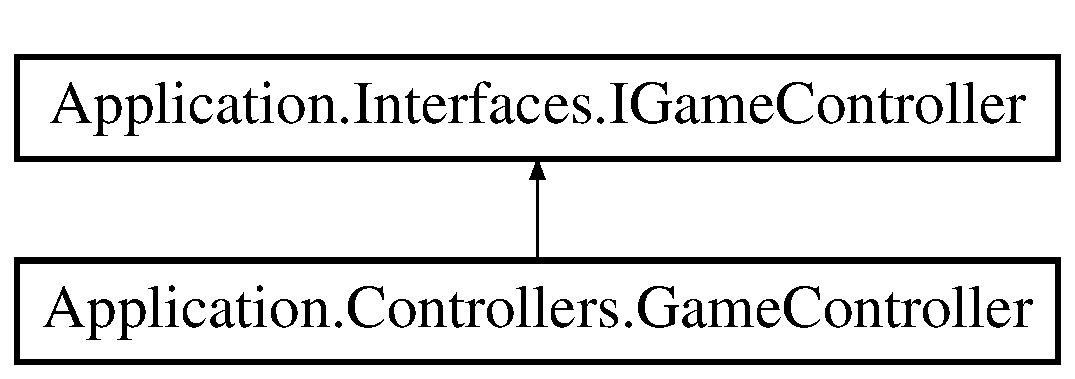
\includegraphics[height=2.000000cm]{class_application_1_1_controllers_1_1_game_controller}
\end{center}
\end{figure}
\subsection*{Public Member Functions}
\begin{DoxyCompactItemize}
\item 
\mbox{\hyperlink{class_application_1_1_controllers_1_1_game_controller_a0576d983a11c3d8f276314ebacece291}{Game\+Controller}} (I\+Game\+Repository game\+Repo)
\item 
void \mbox{\hyperlink{class_application_1_1_controllers_1_1_game_controller_aca897a6c639e043db85b41049d550cf2}{Start\+Game}} (string game\+Id, List$<$ string $>$ playesr\+List)
\begin{DoxyCompactList}\small\item\em starts a game with a Id and a list of player names \end{DoxyCompactList}\item 
I\+Game\+Player\+Info \mbox{\hyperlink{class_application_1_1_controllers_1_1_game_controller_aa0d0e2d74e14771144c1923c77186bb2}{Get\+Players\+Game\+Info}} (string game\+Id, string username)
\item 
bool \mbox{\hyperlink{class_application_1_1_controllers_1_1_game_controller_a5ed6117775253438a76aadcacd44a984}{Leave\+Game}} (string game\+Id, string username)
\end{DoxyCompactItemize}


\subsection{Constructor \& Destructor Documentation}
\mbox{\Hypertarget{class_application_1_1_controllers_1_1_game_controller_a0576d983a11c3d8f276314ebacece291}\label{class_application_1_1_controllers_1_1_game_controller_a0576d983a11c3d8f276314ebacece291}} 
\index{Application\+::\+Controllers\+::\+Game\+Controller@{Application\+::\+Controllers\+::\+Game\+Controller}!Game\+Controller@{Game\+Controller}}
\index{Game\+Controller@{Game\+Controller}!Application\+::\+Controllers\+::\+Game\+Controller@{Application\+::\+Controllers\+::\+Game\+Controller}}
\subsubsection{\texorpdfstring{Game\+Controller()}{GameController()}}
{\footnotesize\ttfamily Application.\+Controllers.\+Game\+Controller.\+Game\+Controller (\begin{DoxyParamCaption}\item[{I\+Game\+Repository}]{game\+Repo }\end{DoxyParamCaption})}



\subsection{Member Function Documentation}
\mbox{\Hypertarget{class_application_1_1_controllers_1_1_game_controller_aa0d0e2d74e14771144c1923c77186bb2}\label{class_application_1_1_controllers_1_1_game_controller_aa0d0e2d74e14771144c1923c77186bb2}} 
\index{Application\+::\+Controllers\+::\+Game\+Controller@{Application\+::\+Controllers\+::\+Game\+Controller}!Get\+Players\+Game\+Info@{Get\+Players\+Game\+Info}}
\index{Get\+Players\+Game\+Info@{Get\+Players\+Game\+Info}!Application\+::\+Controllers\+::\+Game\+Controller@{Application\+::\+Controllers\+::\+Game\+Controller}}
\subsubsection{\texorpdfstring{Get\+Players\+Game\+Info()}{GetPlayersGameInfo()}}
{\footnotesize\ttfamily I\+Game\+Player\+Info Application.\+Controllers.\+Game\+Controller.\+Get\+Players\+Game\+Info (\begin{DoxyParamCaption}\item[{string}]{game\+Id,  }\item[{string}]{username }\end{DoxyParamCaption})}



Implements \mbox{\hyperlink{interface_application_1_1_interfaces_1_1_i_game_controller_a5a0a319e7bbc7c2d4786acf9f78994cb}{Application.\+Interfaces.\+I\+Game\+Controller}}.

\mbox{\Hypertarget{class_application_1_1_controllers_1_1_game_controller_a5ed6117775253438a76aadcacd44a984}\label{class_application_1_1_controllers_1_1_game_controller_a5ed6117775253438a76aadcacd44a984}} 
\index{Application\+::\+Controllers\+::\+Game\+Controller@{Application\+::\+Controllers\+::\+Game\+Controller}!Leave\+Game@{Leave\+Game}}
\index{Leave\+Game@{Leave\+Game}!Application\+::\+Controllers\+::\+Game\+Controller@{Application\+::\+Controllers\+::\+Game\+Controller}}
\subsubsection{\texorpdfstring{Leave\+Game()}{LeaveGame()}}
{\footnotesize\ttfamily bool Application.\+Controllers.\+Game\+Controller.\+Leave\+Game (\begin{DoxyParamCaption}\item[{string}]{game\+Id,  }\item[{string}]{username }\end{DoxyParamCaption})}



Implements \mbox{\hyperlink{interface_application_1_1_interfaces_1_1_i_game_controller_ae81ea4aa4d3146c023277fbf17107623}{Application.\+Interfaces.\+I\+Game\+Controller}}.

\mbox{\Hypertarget{class_application_1_1_controllers_1_1_game_controller_aca897a6c639e043db85b41049d550cf2}\label{class_application_1_1_controllers_1_1_game_controller_aca897a6c639e043db85b41049d550cf2}} 
\index{Application\+::\+Controllers\+::\+Game\+Controller@{Application\+::\+Controllers\+::\+Game\+Controller}!Start\+Game@{Start\+Game}}
\index{Start\+Game@{Start\+Game}!Application\+::\+Controllers\+::\+Game\+Controller@{Application\+::\+Controllers\+::\+Game\+Controller}}
\subsubsection{\texorpdfstring{Start\+Game()}{StartGame()}}
{\footnotesize\ttfamily void Application.\+Controllers.\+Game\+Controller.\+Start\+Game (\begin{DoxyParamCaption}\item[{string}]{game\+Id,  }\item[{List$<$ string $>$}]{playesr\+List }\end{DoxyParamCaption})}



starts a game with a Id and a list of player names 


\begin{DoxyParams}{Parameters}
{\em game\+Id} & \\
\hline
{\em playesr\+List} & \\
\hline
\end{DoxyParams}


Implements \mbox{\hyperlink{interface_application_1_1_interfaces_1_1_i_game_controller_ab3f492a78bbefc5de5dd3de5d1d26f79}{Application.\+Interfaces.\+I\+Game\+Controller}}.



The documentation for this class was generated from the following file\+:\begin{DoxyCompactItemize}
\item 
Controllers/\mbox{\hyperlink{_game_controller_8cs}{Game\+Controller.\+cs}}\end{DoxyCompactItemize}

\hypertarget{interface_application_1_1_misc_1_1_i_cache_handle}{}\section{Application.\+Misc.\+I\+Cache\+Handle Interface Reference}
\label{interface_application_1_1_misc_1_1_i_cache_handle}\index{Application.\+Misc.\+I\+Cache\+Handle@{Application.\+Misc.\+I\+Cache\+Handle}}


The documentation for this interface was generated from the following file\+:\begin{DoxyCompactItemize}
\item 
Misc/\mbox{\hyperlink{_cache_list_8cs}{Cache\+List.\+cs}}\end{DoxyCompactItemize}

\hypertarget{interface_application_1_1_interfaces_1_1_i_game_controller}{}\section{Application.\+Interfaces.\+I\+Game\+Controller Interface Reference}
\label{interface_application_1_1_interfaces_1_1_i_game_controller}\index{Application.\+Interfaces.\+I\+Game\+Controller@{Application.\+Interfaces.\+I\+Game\+Controller}}
Inheritance diagram for Application.\+Interfaces.\+I\+Game\+Controller\+:\begin{figure}[H]
\begin{center}
\leavevmode
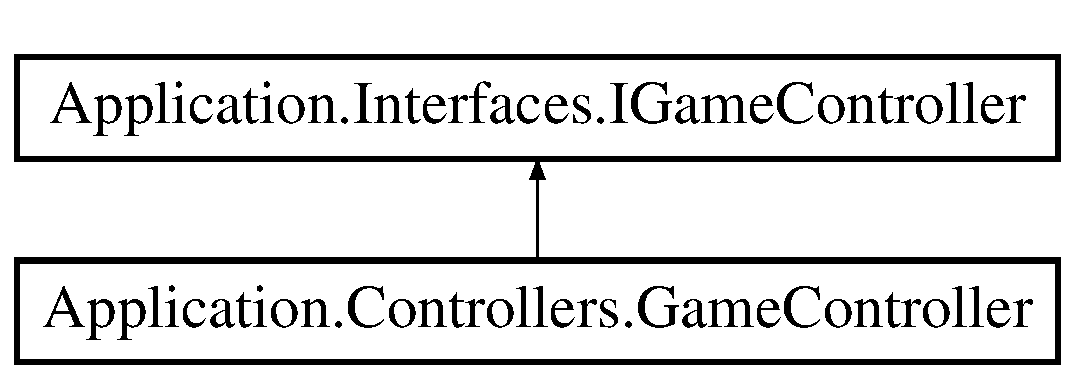
\includegraphics[height=2.000000cm]{interface_application_1_1_interfaces_1_1_i_game_controller}
\end{center}
\end{figure}
\subsection*{Public Member Functions}
\begin{DoxyCompactItemize}
\item 
void \mbox{\hyperlink{interface_application_1_1_interfaces_1_1_i_game_controller_ab3f492a78bbefc5de5dd3de5d1d26f79}{Start\+Game}} (string game\+Id, List$<$ string $>$ playesr\+List)
\begin{DoxyCompactList}\small\item\em starts a game with a Id and a list of player names \end{DoxyCompactList}\item 
I\+Game\+Player\+Info \mbox{\hyperlink{interface_application_1_1_interfaces_1_1_i_game_controller_a5a0a319e7bbc7c2d4786acf9f78994cb}{Get\+Players\+Game\+Info}} (string game\+Id, string username)
\item 
bool \mbox{\hyperlink{interface_application_1_1_interfaces_1_1_i_game_controller_ae81ea4aa4d3146c023277fbf17107623}{Leave\+Game}} (string game\+Id, string username)
\end{DoxyCompactItemize}


\subsection{Member Function Documentation}
\mbox{\Hypertarget{interface_application_1_1_interfaces_1_1_i_game_controller_a5a0a319e7bbc7c2d4786acf9f78994cb}\label{interface_application_1_1_interfaces_1_1_i_game_controller_a5a0a319e7bbc7c2d4786acf9f78994cb}} 
\index{Application\+::\+Interfaces\+::\+I\+Game\+Controller@{Application\+::\+Interfaces\+::\+I\+Game\+Controller}!Get\+Players\+Game\+Info@{Get\+Players\+Game\+Info}}
\index{Get\+Players\+Game\+Info@{Get\+Players\+Game\+Info}!Application\+::\+Interfaces\+::\+I\+Game\+Controller@{Application\+::\+Interfaces\+::\+I\+Game\+Controller}}
\subsubsection{\texorpdfstring{Get\+Players\+Game\+Info()}{GetPlayersGameInfo()}}
{\footnotesize\ttfamily I\+Game\+Player\+Info Application.\+Interfaces.\+I\+Game\+Controller.\+Get\+Players\+Game\+Info (\begin{DoxyParamCaption}\item[{string}]{game\+Id,  }\item[{string}]{username }\end{DoxyParamCaption})}



Implemented in \mbox{\hyperlink{class_application_1_1_controllers_1_1_game_controller_aa0d0e2d74e14771144c1923c77186bb2}{Application.\+Controllers.\+Game\+Controller}}.

\mbox{\Hypertarget{interface_application_1_1_interfaces_1_1_i_game_controller_ae81ea4aa4d3146c023277fbf17107623}\label{interface_application_1_1_interfaces_1_1_i_game_controller_ae81ea4aa4d3146c023277fbf17107623}} 
\index{Application\+::\+Interfaces\+::\+I\+Game\+Controller@{Application\+::\+Interfaces\+::\+I\+Game\+Controller}!Leave\+Game@{Leave\+Game}}
\index{Leave\+Game@{Leave\+Game}!Application\+::\+Interfaces\+::\+I\+Game\+Controller@{Application\+::\+Interfaces\+::\+I\+Game\+Controller}}
\subsubsection{\texorpdfstring{Leave\+Game()}{LeaveGame()}}
{\footnotesize\ttfamily bool Application.\+Interfaces.\+I\+Game\+Controller.\+Leave\+Game (\begin{DoxyParamCaption}\item[{string}]{game\+Id,  }\item[{string}]{username }\end{DoxyParamCaption})}



Implemented in \mbox{\hyperlink{class_application_1_1_controllers_1_1_game_controller_a5ed6117775253438a76aadcacd44a984}{Application.\+Controllers.\+Game\+Controller}}.

\mbox{\Hypertarget{interface_application_1_1_interfaces_1_1_i_game_controller_ab3f492a78bbefc5de5dd3de5d1d26f79}\label{interface_application_1_1_interfaces_1_1_i_game_controller_ab3f492a78bbefc5de5dd3de5d1d26f79}} 
\index{Application\+::\+Interfaces\+::\+I\+Game\+Controller@{Application\+::\+Interfaces\+::\+I\+Game\+Controller}!Start\+Game@{Start\+Game}}
\index{Start\+Game@{Start\+Game}!Application\+::\+Interfaces\+::\+I\+Game\+Controller@{Application\+::\+Interfaces\+::\+I\+Game\+Controller}}
\subsubsection{\texorpdfstring{Start\+Game()}{StartGame()}}
{\footnotesize\ttfamily void Application.\+Interfaces.\+I\+Game\+Controller.\+Start\+Game (\begin{DoxyParamCaption}\item[{string}]{game\+Id,  }\item[{List$<$ string $>$}]{playesr\+List }\end{DoxyParamCaption})}



starts a game with a Id and a list of player names 


\begin{DoxyParams}{Parameters}
{\em game\+Id} & \\
\hline
{\em playesr\+List} & \\
\hline
\end{DoxyParams}


Implemented in \mbox{\hyperlink{class_application_1_1_controllers_1_1_game_controller_aca897a6c639e043db85b41049d550cf2}{Application.\+Controllers.\+Game\+Controller}}.



The documentation for this interface was generated from the following file\+:\begin{DoxyCompactItemize}
\item 
Interfaces/\mbox{\hyperlink{_i_game_controller_8cs}{I\+Game\+Controller.\+cs}}\end{DoxyCompactItemize}

\hypertarget{interface_application_1_1_interfaces_1_1_i_lobby_controller}{}\section{Application.\+Interfaces.\+I\+Lobby\+Controller Interface Reference}
\label{interface_application_1_1_interfaces_1_1_i_lobby_controller}\index{Application.\+Interfaces.\+I\+Lobby\+Controller@{Application.\+Interfaces.\+I\+Lobby\+Controller}}
Inheritance diagram for Application.\+Interfaces.\+I\+Lobby\+Controller\+:\begin{figure}[H]
\begin{center}
\leavevmode
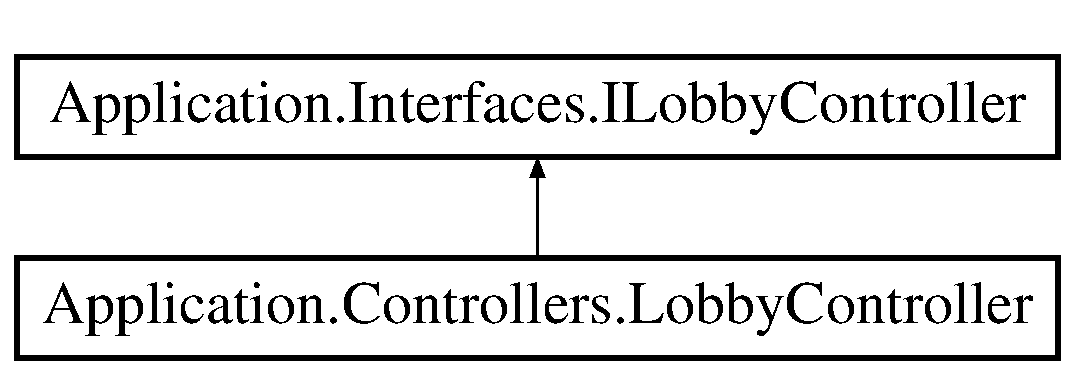
\includegraphics[height=2.000000cm]{interface_application_1_1_interfaces_1_1_i_lobby_controller}
\end{center}
\end{figure}
\subsection*{Public Member Functions}
\begin{DoxyCompactItemize}
\item 
I\+Lobby \mbox{\hyperlink{interface_application_1_1_interfaces_1_1_i_lobby_controller_abefe3510b20e3db41c4d8062f8cdc2bc}{Create\+Lobby}} (string lobby\+Id, string admin\+Username)
\begin{DoxyCompactList}\small\item\em Creates a new lobby and returns this \end{DoxyCompactList}\item 
I\+Lobby \mbox{\hyperlink{interface_application_1_1_interfaces_1_1_i_lobby_controller_a17c37ec6dbb98ab07deb4e4f9800a68e}{Join\+Lobby}} (string lobby\+Id, string username)
\item 
bool \mbox{\hyperlink{interface_application_1_1_interfaces_1_1_i_lobby_controller_ad95e5c656813094f7abec7b81ea568e1}{Leave\+Lobby}} (string lobby\+Id, string username)
\item 
I\+Lobby \mbox{\hyperlink{interface_application_1_1_interfaces_1_1_i_lobby_controller_aaa584fec6fc0e1e0690aa81e7fde3af2}{Get\+Lobby\+By\+Id}} (string lobby\+Id)
\item 
I\+Lobby \mbox{\hyperlink{interface_application_1_1_interfaces_1_1_i_lobby_controller_a4d0618e880423f15785360453bf90f90}{Update\+Lobby}} (string admin\+Username, I\+Lobby lobby)
\begin{DoxyCompactList}\small\item\em Might not be useful. Is meant to update a lobby in scenarios where the admin user wishes to pass on this role to another user. \end{DoxyCompactList}\item 
I\+Collection$<$ string $>$ \mbox{\hyperlink{interface_application_1_1_interfaces_1_1_i_lobby_controller_a2e1d8f72361ee48e956fb473ceabadf4}{Get\+All\+Lobbies}} ()
\item 
Task$<$ I\+Lobby $>$ \mbox{\hyperlink{interface_application_1_1_interfaces_1_1_i_lobby_controller_ae507a1d23088662b8c37692bbb93040e}{Create\+Lobby\+Async}} (string lobby\+Id, string admin\+Username)
\item 
Task$<$ I\+Lobby $>$ \mbox{\hyperlink{interface_application_1_1_interfaces_1_1_i_lobby_controller_aba87a2245b2c274cf977aeaf193eef73}{Join\+Lobby\+Async}} (string lobby\+Id, string username)
\item 
Task$<$ bool $>$ \mbox{\hyperlink{interface_application_1_1_interfaces_1_1_i_lobby_controller_a46975c7e9219d5324f786542a23d9e7e}{Leave\+Lobby\+Async}} (string lobbyid, string username)
\item 
Task$<$ I\+Lobby $>$ \mbox{\hyperlink{interface_application_1_1_interfaces_1_1_i_lobby_controller_a40457a8fb8d6801a8e42f1e75f9d3480}{Update\+Lobby\+Async}} (string admin\+Username, I\+Lobby lobby)
\item 
Task$<$ I\+Collection$<$ string $>$ $>$ \mbox{\hyperlink{interface_application_1_1_interfaces_1_1_i_lobby_controller_acf938121367844d623fa4127cf643e50}{Get\+All\+Lobbies\+Async}} ()
\item 
Task$<$ I\+Lobby $>$ \mbox{\hyperlink{interface_application_1_1_interfaces_1_1_i_lobby_controller_abe3ce90e900391a0c4ffa25195800ab2}{Get\+Lobby\+By\+Id\+Async}} (string lobby\+Id)
\end{DoxyCompactItemize}


\subsection{Member Function Documentation}
\mbox{\Hypertarget{interface_application_1_1_interfaces_1_1_i_lobby_controller_abefe3510b20e3db41c4d8062f8cdc2bc}\label{interface_application_1_1_interfaces_1_1_i_lobby_controller_abefe3510b20e3db41c4d8062f8cdc2bc}} 
\index{Application\+::\+Interfaces\+::\+I\+Lobby\+Controller@{Application\+::\+Interfaces\+::\+I\+Lobby\+Controller}!Create\+Lobby@{Create\+Lobby}}
\index{Create\+Lobby@{Create\+Lobby}!Application\+::\+Interfaces\+::\+I\+Lobby\+Controller@{Application\+::\+Interfaces\+::\+I\+Lobby\+Controller}}
\subsubsection{\texorpdfstring{Create\+Lobby()}{CreateLobby()}}
{\footnotesize\ttfamily I\+Lobby Application.\+Interfaces.\+I\+Lobby\+Controller.\+Create\+Lobby (\begin{DoxyParamCaption}\item[{string}]{lobby\+Id,  }\item[{string}]{admin\+Username }\end{DoxyParamCaption})}



Creates a new lobby and returns this 


\begin{DoxyParams}{Parameters}
{\em lobby\+Id} & The id of the lobby to create\\
\hline
{\em admin\+Username} & The username to be assigned as admin of the lobby\\
\hline
\end{DoxyParams}
\begin{DoxyReturn}{Returns}
Returns a new lobby with the passed information if the lobby id isen\textquotesingle{}t taken and if the user is not currently attached to another lobby. Else null.
\end{DoxyReturn}


Implemented in \mbox{\hyperlink{class_application_1_1_controllers_1_1_lobby_controller_ad0684f9eace44951fcb75c805fb8574c}{Application.\+Controllers.\+Lobby\+Controller}}.

\mbox{\Hypertarget{interface_application_1_1_interfaces_1_1_i_lobby_controller_ae507a1d23088662b8c37692bbb93040e}\label{interface_application_1_1_interfaces_1_1_i_lobby_controller_ae507a1d23088662b8c37692bbb93040e}} 
\index{Application\+::\+Interfaces\+::\+I\+Lobby\+Controller@{Application\+::\+Interfaces\+::\+I\+Lobby\+Controller}!Create\+Lobby\+Async@{Create\+Lobby\+Async}}
\index{Create\+Lobby\+Async@{Create\+Lobby\+Async}!Application\+::\+Interfaces\+::\+I\+Lobby\+Controller@{Application\+::\+Interfaces\+::\+I\+Lobby\+Controller}}
\subsubsection{\texorpdfstring{Create\+Lobby\+Async()}{CreateLobbyAsync()}}
{\footnotesize\ttfamily Task$<$I\+Lobby$>$ Application.\+Interfaces.\+I\+Lobby\+Controller.\+Create\+Lobby\+Async (\begin{DoxyParamCaption}\item[{string}]{lobby\+Id,  }\item[{string}]{admin\+Username }\end{DoxyParamCaption})}



Implemented in \mbox{\hyperlink{class_application_1_1_controllers_1_1_lobby_controller_ac08d941f7da12f7791a691dbbdf0c1f3}{Application.\+Controllers.\+Lobby\+Controller}}.

\mbox{\Hypertarget{interface_application_1_1_interfaces_1_1_i_lobby_controller_a2e1d8f72361ee48e956fb473ceabadf4}\label{interface_application_1_1_interfaces_1_1_i_lobby_controller_a2e1d8f72361ee48e956fb473ceabadf4}} 
\index{Application\+::\+Interfaces\+::\+I\+Lobby\+Controller@{Application\+::\+Interfaces\+::\+I\+Lobby\+Controller}!Get\+All\+Lobbies@{Get\+All\+Lobbies}}
\index{Get\+All\+Lobbies@{Get\+All\+Lobbies}!Application\+::\+Interfaces\+::\+I\+Lobby\+Controller@{Application\+::\+Interfaces\+::\+I\+Lobby\+Controller}}
\subsubsection{\texorpdfstring{Get\+All\+Lobbies()}{GetAllLobbies()}}
{\footnotesize\ttfamily I\+Collection$<$string$>$ Application.\+Interfaces.\+I\+Lobby\+Controller.\+Get\+All\+Lobbies (\begin{DoxyParamCaption}{ }\end{DoxyParamCaption})}



Implemented in \mbox{\hyperlink{class_application_1_1_controllers_1_1_lobby_controller_a1aec115271209fc4ea59ed5f790d3011}{Application.\+Controllers.\+Lobby\+Controller}}.

\mbox{\Hypertarget{interface_application_1_1_interfaces_1_1_i_lobby_controller_acf938121367844d623fa4127cf643e50}\label{interface_application_1_1_interfaces_1_1_i_lobby_controller_acf938121367844d623fa4127cf643e50}} 
\index{Application\+::\+Interfaces\+::\+I\+Lobby\+Controller@{Application\+::\+Interfaces\+::\+I\+Lobby\+Controller}!Get\+All\+Lobbies\+Async@{Get\+All\+Lobbies\+Async}}
\index{Get\+All\+Lobbies\+Async@{Get\+All\+Lobbies\+Async}!Application\+::\+Interfaces\+::\+I\+Lobby\+Controller@{Application\+::\+Interfaces\+::\+I\+Lobby\+Controller}}
\subsubsection{\texorpdfstring{Get\+All\+Lobbies\+Async()}{GetAllLobbiesAsync()}}
{\footnotesize\ttfamily Task$<$I\+Collection$<$string$>$ $>$ Application.\+Interfaces.\+I\+Lobby\+Controller.\+Get\+All\+Lobbies\+Async (\begin{DoxyParamCaption}{ }\end{DoxyParamCaption})}



Implemented in \mbox{\hyperlink{class_application_1_1_controllers_1_1_lobby_controller_a881adadc726a5daa68fe702439723630}{Application.\+Controllers.\+Lobby\+Controller}}.

\mbox{\Hypertarget{interface_application_1_1_interfaces_1_1_i_lobby_controller_aaa584fec6fc0e1e0690aa81e7fde3af2}\label{interface_application_1_1_interfaces_1_1_i_lobby_controller_aaa584fec6fc0e1e0690aa81e7fde3af2}} 
\index{Application\+::\+Interfaces\+::\+I\+Lobby\+Controller@{Application\+::\+Interfaces\+::\+I\+Lobby\+Controller}!Get\+Lobby\+By\+Id@{Get\+Lobby\+By\+Id}}
\index{Get\+Lobby\+By\+Id@{Get\+Lobby\+By\+Id}!Application\+::\+Interfaces\+::\+I\+Lobby\+Controller@{Application\+::\+Interfaces\+::\+I\+Lobby\+Controller}}
\subsubsection{\texorpdfstring{Get\+Lobby\+By\+Id()}{GetLobbyById()}}
{\footnotesize\ttfamily I\+Lobby Application.\+Interfaces.\+I\+Lobby\+Controller.\+Get\+Lobby\+By\+Id (\begin{DoxyParamCaption}\item[{string}]{lobby\+Id }\end{DoxyParamCaption})}



Implemented in \mbox{\hyperlink{class_application_1_1_controllers_1_1_lobby_controller_a5ea797c6456dc8d40e16b87077a16693}{Application.\+Controllers.\+Lobby\+Controller}}.

\mbox{\Hypertarget{interface_application_1_1_interfaces_1_1_i_lobby_controller_abe3ce90e900391a0c4ffa25195800ab2}\label{interface_application_1_1_interfaces_1_1_i_lobby_controller_abe3ce90e900391a0c4ffa25195800ab2}} 
\index{Application\+::\+Interfaces\+::\+I\+Lobby\+Controller@{Application\+::\+Interfaces\+::\+I\+Lobby\+Controller}!Get\+Lobby\+By\+Id\+Async@{Get\+Lobby\+By\+Id\+Async}}
\index{Get\+Lobby\+By\+Id\+Async@{Get\+Lobby\+By\+Id\+Async}!Application\+::\+Interfaces\+::\+I\+Lobby\+Controller@{Application\+::\+Interfaces\+::\+I\+Lobby\+Controller}}
\subsubsection{\texorpdfstring{Get\+Lobby\+By\+Id\+Async()}{GetLobbyByIdAsync()}}
{\footnotesize\ttfamily Task$<$I\+Lobby$>$ Application.\+Interfaces.\+I\+Lobby\+Controller.\+Get\+Lobby\+By\+Id\+Async (\begin{DoxyParamCaption}\item[{string}]{lobby\+Id }\end{DoxyParamCaption})}



Implemented in \mbox{\hyperlink{class_application_1_1_controllers_1_1_lobby_controller_afe14da64961a1667fd7411484204c692}{Application.\+Controllers.\+Lobby\+Controller}}.

\mbox{\Hypertarget{interface_application_1_1_interfaces_1_1_i_lobby_controller_a17c37ec6dbb98ab07deb4e4f9800a68e}\label{interface_application_1_1_interfaces_1_1_i_lobby_controller_a17c37ec6dbb98ab07deb4e4f9800a68e}} 
\index{Application\+::\+Interfaces\+::\+I\+Lobby\+Controller@{Application\+::\+Interfaces\+::\+I\+Lobby\+Controller}!Join\+Lobby@{Join\+Lobby}}
\index{Join\+Lobby@{Join\+Lobby}!Application\+::\+Interfaces\+::\+I\+Lobby\+Controller@{Application\+::\+Interfaces\+::\+I\+Lobby\+Controller}}
\subsubsection{\texorpdfstring{Join\+Lobby()}{JoinLobby()}}
{\footnotesize\ttfamily I\+Lobby Application.\+Interfaces.\+I\+Lobby\+Controller.\+Join\+Lobby (\begin{DoxyParamCaption}\item[{string}]{lobby\+Id,  }\item[{string}]{username }\end{DoxyParamCaption})}



Implemented in \mbox{\hyperlink{class_application_1_1_controllers_1_1_lobby_controller_ac081cab03ea49323b57c294ca95c6a09}{Application.\+Controllers.\+Lobby\+Controller}}.

\mbox{\Hypertarget{interface_application_1_1_interfaces_1_1_i_lobby_controller_aba87a2245b2c274cf977aeaf193eef73}\label{interface_application_1_1_interfaces_1_1_i_lobby_controller_aba87a2245b2c274cf977aeaf193eef73}} 
\index{Application\+::\+Interfaces\+::\+I\+Lobby\+Controller@{Application\+::\+Interfaces\+::\+I\+Lobby\+Controller}!Join\+Lobby\+Async@{Join\+Lobby\+Async}}
\index{Join\+Lobby\+Async@{Join\+Lobby\+Async}!Application\+::\+Interfaces\+::\+I\+Lobby\+Controller@{Application\+::\+Interfaces\+::\+I\+Lobby\+Controller}}
\subsubsection{\texorpdfstring{Join\+Lobby\+Async()}{JoinLobbyAsync()}}
{\footnotesize\ttfamily Task$<$I\+Lobby$>$ Application.\+Interfaces.\+I\+Lobby\+Controller.\+Join\+Lobby\+Async (\begin{DoxyParamCaption}\item[{string}]{lobby\+Id,  }\item[{string}]{username }\end{DoxyParamCaption})}



Implemented in \mbox{\hyperlink{class_application_1_1_controllers_1_1_lobby_controller_af9484a4c054717c0975175d93e45149c}{Application.\+Controllers.\+Lobby\+Controller}}.

\mbox{\Hypertarget{interface_application_1_1_interfaces_1_1_i_lobby_controller_ad95e5c656813094f7abec7b81ea568e1}\label{interface_application_1_1_interfaces_1_1_i_lobby_controller_ad95e5c656813094f7abec7b81ea568e1}} 
\index{Application\+::\+Interfaces\+::\+I\+Lobby\+Controller@{Application\+::\+Interfaces\+::\+I\+Lobby\+Controller}!Leave\+Lobby@{Leave\+Lobby}}
\index{Leave\+Lobby@{Leave\+Lobby}!Application\+::\+Interfaces\+::\+I\+Lobby\+Controller@{Application\+::\+Interfaces\+::\+I\+Lobby\+Controller}}
\subsubsection{\texorpdfstring{Leave\+Lobby()}{LeaveLobby()}}
{\footnotesize\ttfamily bool Application.\+Interfaces.\+I\+Lobby\+Controller.\+Leave\+Lobby (\begin{DoxyParamCaption}\item[{string}]{lobby\+Id,  }\item[{string}]{username }\end{DoxyParamCaption})}



Implemented in \mbox{\hyperlink{class_application_1_1_controllers_1_1_lobby_controller_aa075018713d8ac7fdf84cf6349e2f10d}{Application.\+Controllers.\+Lobby\+Controller}}.

\mbox{\Hypertarget{interface_application_1_1_interfaces_1_1_i_lobby_controller_a46975c7e9219d5324f786542a23d9e7e}\label{interface_application_1_1_interfaces_1_1_i_lobby_controller_a46975c7e9219d5324f786542a23d9e7e}} 
\index{Application\+::\+Interfaces\+::\+I\+Lobby\+Controller@{Application\+::\+Interfaces\+::\+I\+Lobby\+Controller}!Leave\+Lobby\+Async@{Leave\+Lobby\+Async}}
\index{Leave\+Lobby\+Async@{Leave\+Lobby\+Async}!Application\+::\+Interfaces\+::\+I\+Lobby\+Controller@{Application\+::\+Interfaces\+::\+I\+Lobby\+Controller}}
\subsubsection{\texorpdfstring{Leave\+Lobby\+Async()}{LeaveLobbyAsync()}}
{\footnotesize\ttfamily Task$<$bool$>$ Application.\+Interfaces.\+I\+Lobby\+Controller.\+Leave\+Lobby\+Async (\begin{DoxyParamCaption}\item[{string}]{lobbyid,  }\item[{string}]{username }\end{DoxyParamCaption})}



Implemented in \mbox{\hyperlink{class_application_1_1_controllers_1_1_lobby_controller_a7f0fb3932a42b76d5e4a9788aa0510e0}{Application.\+Controllers.\+Lobby\+Controller}}.

\mbox{\Hypertarget{interface_application_1_1_interfaces_1_1_i_lobby_controller_a4d0618e880423f15785360453bf90f90}\label{interface_application_1_1_interfaces_1_1_i_lobby_controller_a4d0618e880423f15785360453bf90f90}} 
\index{Application\+::\+Interfaces\+::\+I\+Lobby\+Controller@{Application\+::\+Interfaces\+::\+I\+Lobby\+Controller}!Update\+Lobby@{Update\+Lobby}}
\index{Update\+Lobby@{Update\+Lobby}!Application\+::\+Interfaces\+::\+I\+Lobby\+Controller@{Application\+::\+Interfaces\+::\+I\+Lobby\+Controller}}
\subsubsection{\texorpdfstring{Update\+Lobby()}{UpdateLobby()}}
{\footnotesize\ttfamily I\+Lobby Application.\+Interfaces.\+I\+Lobby\+Controller.\+Update\+Lobby (\begin{DoxyParamCaption}\item[{string}]{admin\+Username,  }\item[{I\+Lobby}]{lobby }\end{DoxyParamCaption})}



Might not be useful. Is meant to update a lobby in scenarios where the admin user wishes to pass on this role to another user. 


\begin{DoxyParams}{Parameters}
{\em admin\+Username} & Username of the current admin of the passed \mbox{\hyperlink{}{I\+Lobby}} lobby\\
\hline
{\em lobby} & The lobby to update\\
\hline
\end{DoxyParams}
\begin{DoxyReturn}{Returns}
The updated lobby upon succes. Else null.
\end{DoxyReturn}


Implemented in \mbox{\hyperlink{class_application_1_1_controllers_1_1_lobby_controller_a415b61b5c78ba52619ac4d3606ecc32e}{Application.\+Controllers.\+Lobby\+Controller}}.

\mbox{\Hypertarget{interface_application_1_1_interfaces_1_1_i_lobby_controller_a40457a8fb8d6801a8e42f1e75f9d3480}\label{interface_application_1_1_interfaces_1_1_i_lobby_controller_a40457a8fb8d6801a8e42f1e75f9d3480}} 
\index{Application\+::\+Interfaces\+::\+I\+Lobby\+Controller@{Application\+::\+Interfaces\+::\+I\+Lobby\+Controller}!Update\+Lobby\+Async@{Update\+Lobby\+Async}}
\index{Update\+Lobby\+Async@{Update\+Lobby\+Async}!Application\+::\+Interfaces\+::\+I\+Lobby\+Controller@{Application\+::\+Interfaces\+::\+I\+Lobby\+Controller}}
\subsubsection{\texorpdfstring{Update\+Lobby\+Async()}{UpdateLobbyAsync()}}
{\footnotesize\ttfamily Task$<$I\+Lobby$>$ Application.\+Interfaces.\+I\+Lobby\+Controller.\+Update\+Lobby\+Async (\begin{DoxyParamCaption}\item[{string}]{admin\+Username,  }\item[{I\+Lobby}]{lobby }\end{DoxyParamCaption})}



Implemented in \mbox{\hyperlink{class_application_1_1_controllers_1_1_lobby_controller_a2f30842e0480f28ddbe51ab420b35049}{Application.\+Controllers.\+Lobby\+Controller}}.



The documentation for this interface was generated from the following file\+:\begin{DoxyCompactItemize}
\item 
Interfaces/\mbox{\hyperlink{_i_lobby_controller_8cs}{I\+Lobby\+Controller.\+cs}}\end{DoxyCompactItemize}

\hypertarget{interface_application_1_1_interfaces_1_1_i_lobby_pool}{}\section{Application.\+Interfaces.\+I\+Lobby\+Pool Interface Reference}
\label{interface_application_1_1_interfaces_1_1_i_lobby_pool}\index{Application.\+Interfaces.\+I\+Lobby\+Pool@{Application.\+Interfaces.\+I\+Lobby\+Pool}}
Inheritance diagram for Application.\+Interfaces.\+I\+Lobby\+Pool\+:\begin{figure}[H]
\begin{center}
\leavevmode
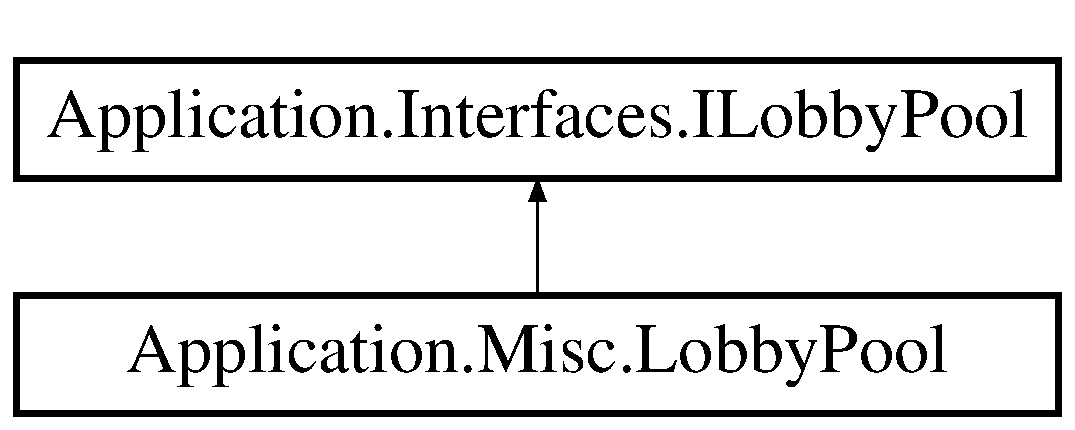
\includegraphics[height=2.000000cm]{interface_application_1_1_interfaces_1_1_i_lobby_pool}
\end{center}
\end{figure}
\subsection*{Public Member Functions}
\begin{DoxyCompactItemize}
\item 
I\+Lobby \mbox{\hyperlink{interface_application_1_1_interfaces_1_1_i_lobby_pool_a044d19c090cbd70a17de4b487fd6d613}{Get\+Lobby}} (string lobby\+Id)
\item 
bool \mbox{\hyperlink{interface_application_1_1_interfaces_1_1_i_lobby_pool_a2aa933d501630b665f67c68e39012a4c}{Add\+Lobby}} (I\+Lobby lobby)
\item 
bool \mbox{\hyperlink{interface_application_1_1_interfaces_1_1_i_lobby_pool_a61058848af185e20841421e7f52e8b94}{Release\+Lobby}} (string lobby\+Id)
\item 
bool \mbox{\hyperlink{interface_application_1_1_interfaces_1_1_i_lobby_pool_a9a09df8415ae760c99d5a6bcd1ac91f9}{Contains}} (string lobby\+Id)
\item 
I\+Enumerable$<$ I\+Lobby $>$ \mbox{\hyperlink{interface_application_1_1_interfaces_1_1_i_lobby_pool_ac64adf71b4ab967725dec520bab627c3}{Find}} (Func$<$ I\+Lobby, bool $>$ func)
\item 
I\+Lobby \mbox{\hyperlink{interface_application_1_1_interfaces_1_1_i_lobby_pool_aa518351cc8b58ef5997f7ecef19633bb}{First\+Or\+Default}} (Func$<$ I\+Lobby, bool $>$ func)
\end{DoxyCompactItemize}
\subsection*{Properties}
\begin{DoxyCompactItemize}
\item 
I\+Collection$<$ string $>$ \mbox{\hyperlink{interface_application_1_1_interfaces_1_1_i_lobby_pool_acbba38f6800479622a56b3347bbd1f63}{Lobbies\+Collection}}\hspace{0.3cm}{\ttfamily  \mbox{[}get\mbox{]}}
\end{DoxyCompactItemize}


\subsection{Member Function Documentation}
\mbox{\Hypertarget{interface_application_1_1_interfaces_1_1_i_lobby_pool_a2aa933d501630b665f67c68e39012a4c}\label{interface_application_1_1_interfaces_1_1_i_lobby_pool_a2aa933d501630b665f67c68e39012a4c}} 
\index{Application\+::\+Interfaces\+::\+I\+Lobby\+Pool@{Application\+::\+Interfaces\+::\+I\+Lobby\+Pool}!Add\+Lobby@{Add\+Lobby}}
\index{Add\+Lobby@{Add\+Lobby}!Application\+::\+Interfaces\+::\+I\+Lobby\+Pool@{Application\+::\+Interfaces\+::\+I\+Lobby\+Pool}}
\subsubsection{\texorpdfstring{Add\+Lobby()}{AddLobby()}}
{\footnotesize\ttfamily bool Application.\+Interfaces.\+I\+Lobby\+Pool.\+Add\+Lobby (\begin{DoxyParamCaption}\item[{I\+Lobby}]{lobby }\end{DoxyParamCaption})}



Implemented in \mbox{\hyperlink{class_application_1_1_misc_1_1_lobby_pool_a442eb666b16bc75025732413f38b0846}{Application.\+Misc.\+Lobby\+Pool}}.

\mbox{\Hypertarget{interface_application_1_1_interfaces_1_1_i_lobby_pool_a9a09df8415ae760c99d5a6bcd1ac91f9}\label{interface_application_1_1_interfaces_1_1_i_lobby_pool_a9a09df8415ae760c99d5a6bcd1ac91f9}} 
\index{Application\+::\+Interfaces\+::\+I\+Lobby\+Pool@{Application\+::\+Interfaces\+::\+I\+Lobby\+Pool}!Contains@{Contains}}
\index{Contains@{Contains}!Application\+::\+Interfaces\+::\+I\+Lobby\+Pool@{Application\+::\+Interfaces\+::\+I\+Lobby\+Pool}}
\subsubsection{\texorpdfstring{Contains()}{Contains()}}
{\footnotesize\ttfamily bool Application.\+Interfaces.\+I\+Lobby\+Pool.\+Contains (\begin{DoxyParamCaption}\item[{string}]{lobby\+Id }\end{DoxyParamCaption})}



Implemented in \mbox{\hyperlink{class_application_1_1_misc_1_1_lobby_pool_af9f3a5b65c1a948fa63796a907c1684d}{Application.\+Misc.\+Lobby\+Pool}}.

\mbox{\Hypertarget{interface_application_1_1_interfaces_1_1_i_lobby_pool_ac64adf71b4ab967725dec520bab627c3}\label{interface_application_1_1_interfaces_1_1_i_lobby_pool_ac64adf71b4ab967725dec520bab627c3}} 
\index{Application\+::\+Interfaces\+::\+I\+Lobby\+Pool@{Application\+::\+Interfaces\+::\+I\+Lobby\+Pool}!Find@{Find}}
\index{Find@{Find}!Application\+::\+Interfaces\+::\+I\+Lobby\+Pool@{Application\+::\+Interfaces\+::\+I\+Lobby\+Pool}}
\subsubsection{\texorpdfstring{Find()}{Find()}}
{\footnotesize\ttfamily I\+Enumerable$<$I\+Lobby$>$ Application.\+Interfaces.\+I\+Lobby\+Pool.\+Find (\begin{DoxyParamCaption}\item[{Func$<$ I\+Lobby, bool $>$}]{func }\end{DoxyParamCaption})}



Implemented in \mbox{\hyperlink{class_application_1_1_misc_1_1_lobby_pool_a3d1c9e496386713ad5d8ede307e6c28c}{Application.\+Misc.\+Lobby\+Pool}}.

\mbox{\Hypertarget{interface_application_1_1_interfaces_1_1_i_lobby_pool_aa518351cc8b58ef5997f7ecef19633bb}\label{interface_application_1_1_interfaces_1_1_i_lobby_pool_aa518351cc8b58ef5997f7ecef19633bb}} 
\index{Application\+::\+Interfaces\+::\+I\+Lobby\+Pool@{Application\+::\+Interfaces\+::\+I\+Lobby\+Pool}!First\+Or\+Default@{First\+Or\+Default}}
\index{First\+Or\+Default@{First\+Or\+Default}!Application\+::\+Interfaces\+::\+I\+Lobby\+Pool@{Application\+::\+Interfaces\+::\+I\+Lobby\+Pool}}
\subsubsection{\texorpdfstring{First\+Or\+Default()}{FirstOrDefault()}}
{\footnotesize\ttfamily I\+Lobby Application.\+Interfaces.\+I\+Lobby\+Pool.\+First\+Or\+Default (\begin{DoxyParamCaption}\item[{Func$<$ I\+Lobby, bool $>$}]{func }\end{DoxyParamCaption})}



Implemented in \mbox{\hyperlink{class_application_1_1_misc_1_1_lobby_pool_a5676f006bc10c46224c1b3bb266702a3}{Application.\+Misc.\+Lobby\+Pool}}.

\mbox{\Hypertarget{interface_application_1_1_interfaces_1_1_i_lobby_pool_a044d19c090cbd70a17de4b487fd6d613}\label{interface_application_1_1_interfaces_1_1_i_lobby_pool_a044d19c090cbd70a17de4b487fd6d613}} 
\index{Application\+::\+Interfaces\+::\+I\+Lobby\+Pool@{Application\+::\+Interfaces\+::\+I\+Lobby\+Pool}!Get\+Lobby@{Get\+Lobby}}
\index{Get\+Lobby@{Get\+Lobby}!Application\+::\+Interfaces\+::\+I\+Lobby\+Pool@{Application\+::\+Interfaces\+::\+I\+Lobby\+Pool}}
\subsubsection{\texorpdfstring{Get\+Lobby()}{GetLobby()}}
{\footnotesize\ttfamily I\+Lobby Application.\+Interfaces.\+I\+Lobby\+Pool.\+Get\+Lobby (\begin{DoxyParamCaption}\item[{string}]{lobby\+Id }\end{DoxyParamCaption})}



Implemented in \mbox{\hyperlink{class_application_1_1_misc_1_1_lobby_pool_a61b2a303bd4bc1e72e31b3ee3d1e06d5}{Application.\+Misc.\+Lobby\+Pool}}.

\mbox{\Hypertarget{interface_application_1_1_interfaces_1_1_i_lobby_pool_a61058848af185e20841421e7f52e8b94}\label{interface_application_1_1_interfaces_1_1_i_lobby_pool_a61058848af185e20841421e7f52e8b94}} 
\index{Application\+::\+Interfaces\+::\+I\+Lobby\+Pool@{Application\+::\+Interfaces\+::\+I\+Lobby\+Pool}!Release\+Lobby@{Release\+Lobby}}
\index{Release\+Lobby@{Release\+Lobby}!Application\+::\+Interfaces\+::\+I\+Lobby\+Pool@{Application\+::\+Interfaces\+::\+I\+Lobby\+Pool}}
\subsubsection{\texorpdfstring{Release\+Lobby()}{ReleaseLobby()}}
{\footnotesize\ttfamily bool Application.\+Interfaces.\+I\+Lobby\+Pool.\+Release\+Lobby (\begin{DoxyParamCaption}\item[{string}]{lobby\+Id }\end{DoxyParamCaption})}



Implemented in \mbox{\hyperlink{class_application_1_1_misc_1_1_lobby_pool_a747cfa417f8932fa8b006b6662c45099}{Application.\+Misc.\+Lobby\+Pool}}.



\subsection{Property Documentation}
\mbox{\Hypertarget{interface_application_1_1_interfaces_1_1_i_lobby_pool_acbba38f6800479622a56b3347bbd1f63}\label{interface_application_1_1_interfaces_1_1_i_lobby_pool_acbba38f6800479622a56b3347bbd1f63}} 
\index{Application\+::\+Interfaces\+::\+I\+Lobby\+Pool@{Application\+::\+Interfaces\+::\+I\+Lobby\+Pool}!Lobbies\+Collection@{Lobbies\+Collection}}
\index{Lobbies\+Collection@{Lobbies\+Collection}!Application\+::\+Interfaces\+::\+I\+Lobby\+Pool@{Application\+::\+Interfaces\+::\+I\+Lobby\+Pool}}
\subsubsection{\texorpdfstring{Lobbies\+Collection}{LobbiesCollection}}
{\footnotesize\ttfamily I\+Collection$<$string$>$ Application.\+Interfaces.\+I\+Lobby\+Pool.\+Lobbies\+Collection\hspace{0.3cm}{\ttfamily [get]}}



The documentation for this interface was generated from the following file\+:\begin{DoxyCompactItemize}
\item 
Interfaces/\mbox{\hyperlink{_i_lobby_pool_8cs}{I\+Lobby\+Pool.\+cs}}\end{DoxyCompactItemize}

\hypertarget{interface_application_1_1_interfaces_1_1_i_login_manager}{}\section{Application.\+Interfaces.\+I\+Login\+Manager Interface Reference}
\label{interface_application_1_1_interfaces_1_1_i_login_manager}\index{Application.\+Interfaces.\+I\+Login\+Manager@{Application.\+Interfaces.\+I\+Login\+Manager}}
Inheritance diagram for Application.\+Interfaces.\+I\+Login\+Manager\+:\begin{figure}[H]
\begin{center}
\leavevmode
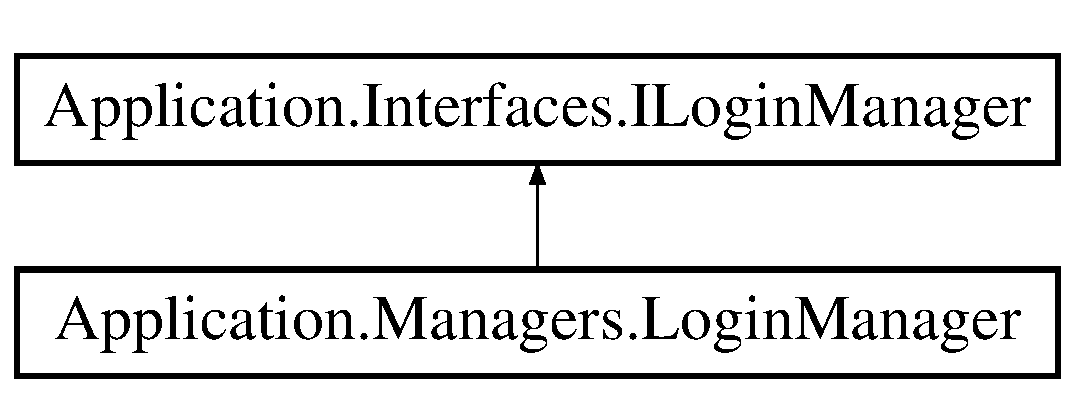
\includegraphics[height=2.000000cm]{interface_application_1_1_interfaces_1_1_i_login_manager}
\end{center}
\end{figure}
\subsection*{Public Member Functions}
\begin{DoxyCompactItemize}
\item 
void \mbox{\hyperlink{interface_application_1_1_interfaces_1_1_i_login_manager_abfad12b55f211087464278f6301ba2e6}{Login}} (I\+User user)
\begin{DoxyCompactList}\small\item\em Logs in the user \end{DoxyCompactList}\item 
bool \mbox{\hyperlink{interface_application_1_1_interfaces_1_1_i_login_manager_a31282ac878dc798af1a542f23efc7c8b}{Check\+Login\+Status}} (string username, string password)
\begin{DoxyCompactList}\small\item\em Returns whether the user with username is logged in. If this is the case it updates the users time stamp \end{DoxyCompactList}\item 
bool \mbox{\hyperlink{interface_application_1_1_interfaces_1_1_i_login_manager_a81fc028c701e8e372d635d6bd9664570}{Subscribe\+On\+Log\+Out}} (string username, \mbox{\hyperlink{namespace_application_1_1_interfaces_a3ba96a057acca29f3e2e533aeb2f30e0}{User\+Logged\+Out\+Handle}} handle)
\begin{DoxyCompactList}\small\item\em Subscribe to the username with the given handler. If the user is logged out the handler will get called. Make sure to call Check\+Login\+Status prior to this call \end{DoxyCompactList}\item 
bool \mbox{\hyperlink{interface_application_1_1_interfaces_1_1_i_login_manager_aeb60a7935fa777e629db6098ce2f458d}{Unsubscribe\+On\+Log\+Out}} (string username, \mbox{\hyperlink{namespace_application_1_1_interfaces_a3ba96a057acca29f3e2e533aeb2f30e0}{User\+Logged\+Out\+Handle}} handle)
\begin{DoxyCompactList}\small\item\em Unsubscribes the handler from the username. \end{DoxyCompactList}\end{DoxyCompactItemize}


\subsection{Member Function Documentation}
\mbox{\Hypertarget{interface_application_1_1_interfaces_1_1_i_login_manager_a31282ac878dc798af1a542f23efc7c8b}\label{interface_application_1_1_interfaces_1_1_i_login_manager_a31282ac878dc798af1a542f23efc7c8b}} 
\index{Application\+::\+Interfaces\+::\+I\+Login\+Manager@{Application\+::\+Interfaces\+::\+I\+Login\+Manager}!Check\+Login\+Status@{Check\+Login\+Status}}
\index{Check\+Login\+Status@{Check\+Login\+Status}!Application\+::\+Interfaces\+::\+I\+Login\+Manager@{Application\+::\+Interfaces\+::\+I\+Login\+Manager}}
\subsubsection{\texorpdfstring{Check\+Login\+Status()}{CheckLoginStatus()}}
{\footnotesize\ttfamily bool Application.\+Interfaces.\+I\+Login\+Manager.\+Check\+Login\+Status (\begin{DoxyParamCaption}\item[{string}]{username,  }\item[{string}]{password }\end{DoxyParamCaption})}



Returns whether the user with username is logged in. If this is the case it updates the users time stamp 


\begin{DoxyParams}{Parameters}
{\em username} & \\
\hline
\end{DoxyParams}
\begin{DoxyReturn}{Returns}

\end{DoxyReturn}


Implemented in \mbox{\hyperlink{class_application_1_1_managers_1_1_login_manager_ab485bd570a5d994461c54eb07e97a43a}{Application.\+Managers.\+Login\+Manager}}.

\mbox{\Hypertarget{interface_application_1_1_interfaces_1_1_i_login_manager_abfad12b55f211087464278f6301ba2e6}\label{interface_application_1_1_interfaces_1_1_i_login_manager_abfad12b55f211087464278f6301ba2e6}} 
\index{Application\+::\+Interfaces\+::\+I\+Login\+Manager@{Application\+::\+Interfaces\+::\+I\+Login\+Manager}!Login@{Login}}
\index{Login@{Login}!Application\+::\+Interfaces\+::\+I\+Login\+Manager@{Application\+::\+Interfaces\+::\+I\+Login\+Manager}}
\subsubsection{\texorpdfstring{Login()}{Login()}}
{\footnotesize\ttfamily void Application.\+Interfaces.\+I\+Login\+Manager.\+Login (\begin{DoxyParamCaption}\item[{I\+User}]{user }\end{DoxyParamCaption})}



Logs in the user 


\begin{DoxyParams}{Parameters}
{\em user} & \\
\hline
\end{DoxyParams}


Implemented in \mbox{\hyperlink{class_application_1_1_managers_1_1_login_manager_a561516fbf8f97f695efdb1cb696899e8}{Application.\+Managers.\+Login\+Manager}}.

\mbox{\Hypertarget{interface_application_1_1_interfaces_1_1_i_login_manager_a81fc028c701e8e372d635d6bd9664570}\label{interface_application_1_1_interfaces_1_1_i_login_manager_a81fc028c701e8e372d635d6bd9664570}} 
\index{Application\+::\+Interfaces\+::\+I\+Login\+Manager@{Application\+::\+Interfaces\+::\+I\+Login\+Manager}!Subscribe\+On\+Log\+Out@{Subscribe\+On\+Log\+Out}}
\index{Subscribe\+On\+Log\+Out@{Subscribe\+On\+Log\+Out}!Application\+::\+Interfaces\+::\+I\+Login\+Manager@{Application\+::\+Interfaces\+::\+I\+Login\+Manager}}
\subsubsection{\texorpdfstring{Subscribe\+On\+Log\+Out()}{SubscribeOnLogOut()}}
{\footnotesize\ttfamily bool Application.\+Interfaces.\+I\+Login\+Manager.\+Subscribe\+On\+Log\+Out (\begin{DoxyParamCaption}\item[{string}]{username,  }\item[{\mbox{\hyperlink{namespace_application_1_1_interfaces_a3ba96a057acca29f3e2e533aeb2f30e0}{User\+Logged\+Out\+Handle}}}]{handle }\end{DoxyParamCaption})}



Subscribe to the username with the given handler. If the user is logged out the handler will get called. Make sure to call Check\+Login\+Status prior to this call 


\begin{DoxyParams}{Parameters}
{\em username} & \\
\hline
{\em handle} & \\
\hline
\end{DoxyParams}
\begin{DoxyReturn}{Returns}

\end{DoxyReturn}


Implemented in \mbox{\hyperlink{class_application_1_1_managers_1_1_login_manager_a9502ab9e9e8d04a42a9c3cdf451b405b}{Application.\+Managers.\+Login\+Manager}}.

\mbox{\Hypertarget{interface_application_1_1_interfaces_1_1_i_login_manager_aeb60a7935fa777e629db6098ce2f458d}\label{interface_application_1_1_interfaces_1_1_i_login_manager_aeb60a7935fa777e629db6098ce2f458d}} 
\index{Application\+::\+Interfaces\+::\+I\+Login\+Manager@{Application\+::\+Interfaces\+::\+I\+Login\+Manager}!Unsubscribe\+On\+Log\+Out@{Unsubscribe\+On\+Log\+Out}}
\index{Unsubscribe\+On\+Log\+Out@{Unsubscribe\+On\+Log\+Out}!Application\+::\+Interfaces\+::\+I\+Login\+Manager@{Application\+::\+Interfaces\+::\+I\+Login\+Manager}}
\subsubsection{\texorpdfstring{Unsubscribe\+On\+Log\+Out()}{UnsubscribeOnLogOut()}}
{\footnotesize\ttfamily bool Application.\+Interfaces.\+I\+Login\+Manager.\+Unsubscribe\+On\+Log\+Out (\begin{DoxyParamCaption}\item[{string}]{username,  }\item[{\mbox{\hyperlink{namespace_application_1_1_interfaces_a3ba96a057acca29f3e2e533aeb2f30e0}{User\+Logged\+Out\+Handle}}}]{handle }\end{DoxyParamCaption})}



Unsubscribes the handler from the username. 


\begin{DoxyParams}{Parameters}
{\em username} & \\
\hline
{\em handle} & \\
\hline
\end{DoxyParams}
\begin{DoxyReturn}{Returns}

\end{DoxyReturn}


Implemented in \mbox{\hyperlink{class_application_1_1_managers_1_1_login_manager_a4490bbdc301ad6eab762fd1a567fd970}{Application.\+Managers.\+Login\+Manager}}.



The documentation for this interface was generated from the following file\+:\begin{DoxyCompactItemize}
\item 
Interfaces/\mbox{\hyperlink{_i_login_manager_8cs}{I\+Login\+Manager.\+cs}}\end{DoxyCompactItemize}

\hypertarget{interface_application_1_1_interfaces_1_1_i_timer}{}\section{Application.\+Interfaces.\+I\+Timer Interface Reference}
\label{interface_application_1_1_interfaces_1_1_i_timer}\index{Application.\+Interfaces.\+I\+Timer@{Application.\+Interfaces.\+I\+Timer}}
Inheritance diagram for Application.\+Interfaces.\+I\+Timer\+:\begin{figure}[H]
\begin{center}
\leavevmode
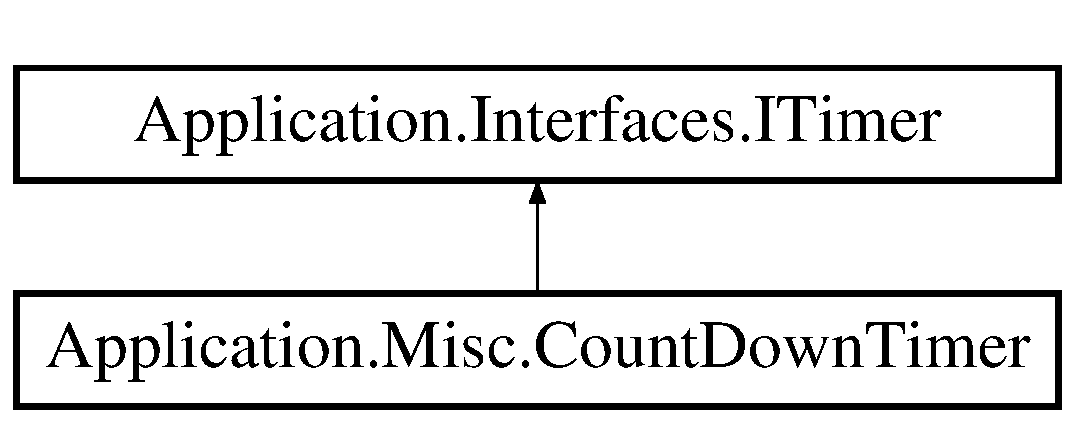
\includegraphics[height=2.000000cm]{interface_application_1_1_interfaces_1_1_i_timer}
\end{center}
\end{figure}
\subsection*{Public Member Functions}
\begin{DoxyCompactItemize}
\item 
void \mbox{\hyperlink{interface_application_1_1_interfaces_1_1_i_timer_a220100133da4e47f2a1654966f33e9e6}{Start\+With\+Seconds}} (int seconds)
\item 
void \mbox{\hyperlink{interface_application_1_1_interfaces_1_1_i_timer_af2759fd575f1ae0a8df31f753bfeaf07}{Start\+With\+Minutes}} (int minutes)
\item 
void \mbox{\hyperlink{interface_application_1_1_interfaces_1_1_i_timer_a127e73defb495fef00e24cdc0f73936e}{Start}} (int minutes, int seconds)
\item 
void \mbox{\hyperlink{interface_application_1_1_interfaces_1_1_i_timer_a20bbfb25ff2343e0d3ea4b6ea708af90}{Stop}} ()
\end{DoxyCompactItemize}
\subsection*{Events}
\begin{DoxyCompactItemize}
\item 
Event\+Handler \mbox{\hyperlink{interface_application_1_1_interfaces_1_1_i_timer_af8955cf4dc8aa8183653cb62b713defd}{Tick\+Event}}
\item 
Event\+Handler \mbox{\hyperlink{interface_application_1_1_interfaces_1_1_i_timer_a0deff851942159fe368552fbeeaa3686}{Expired\+Event}}
\end{DoxyCompactItemize}


\subsection{Member Function Documentation}
\mbox{\Hypertarget{interface_application_1_1_interfaces_1_1_i_timer_a127e73defb495fef00e24cdc0f73936e}\label{interface_application_1_1_interfaces_1_1_i_timer_a127e73defb495fef00e24cdc0f73936e}} 
\index{Application\+::\+Interfaces\+::\+I\+Timer@{Application\+::\+Interfaces\+::\+I\+Timer}!Start@{Start}}
\index{Start@{Start}!Application\+::\+Interfaces\+::\+I\+Timer@{Application\+::\+Interfaces\+::\+I\+Timer}}
\subsubsection{\texorpdfstring{Start()}{Start()}}
{\footnotesize\ttfamily void Application.\+Interfaces.\+I\+Timer.\+Start (\begin{DoxyParamCaption}\item[{int}]{minutes,  }\item[{int}]{seconds }\end{DoxyParamCaption})}



Implemented in \mbox{\hyperlink{class_application_1_1_misc_1_1_count_down_timer_a287fe196667f4c6aca7fb14506f14916}{Application.\+Misc.\+Count\+Down\+Timer}}.

\mbox{\Hypertarget{interface_application_1_1_interfaces_1_1_i_timer_af2759fd575f1ae0a8df31f753bfeaf07}\label{interface_application_1_1_interfaces_1_1_i_timer_af2759fd575f1ae0a8df31f753bfeaf07}} 
\index{Application\+::\+Interfaces\+::\+I\+Timer@{Application\+::\+Interfaces\+::\+I\+Timer}!Start\+With\+Minutes@{Start\+With\+Minutes}}
\index{Start\+With\+Minutes@{Start\+With\+Minutes}!Application\+::\+Interfaces\+::\+I\+Timer@{Application\+::\+Interfaces\+::\+I\+Timer}}
\subsubsection{\texorpdfstring{Start\+With\+Minutes()}{StartWithMinutes()}}
{\footnotesize\ttfamily void Application.\+Interfaces.\+I\+Timer.\+Start\+With\+Minutes (\begin{DoxyParamCaption}\item[{int}]{minutes }\end{DoxyParamCaption})}



Implemented in \mbox{\hyperlink{class_application_1_1_misc_1_1_count_down_timer_a46a066ed728519a096d6e47a9df080a3}{Application.\+Misc.\+Count\+Down\+Timer}}.

\mbox{\Hypertarget{interface_application_1_1_interfaces_1_1_i_timer_a220100133da4e47f2a1654966f33e9e6}\label{interface_application_1_1_interfaces_1_1_i_timer_a220100133da4e47f2a1654966f33e9e6}} 
\index{Application\+::\+Interfaces\+::\+I\+Timer@{Application\+::\+Interfaces\+::\+I\+Timer}!Start\+With\+Seconds@{Start\+With\+Seconds}}
\index{Start\+With\+Seconds@{Start\+With\+Seconds}!Application\+::\+Interfaces\+::\+I\+Timer@{Application\+::\+Interfaces\+::\+I\+Timer}}
\subsubsection{\texorpdfstring{Start\+With\+Seconds()}{StartWithSeconds()}}
{\footnotesize\ttfamily void Application.\+Interfaces.\+I\+Timer.\+Start\+With\+Seconds (\begin{DoxyParamCaption}\item[{int}]{seconds }\end{DoxyParamCaption})}



Implemented in \mbox{\hyperlink{class_application_1_1_misc_1_1_count_down_timer_ad07500432508a81df8f19fc55da7fc27}{Application.\+Misc.\+Count\+Down\+Timer}}.

\mbox{\Hypertarget{interface_application_1_1_interfaces_1_1_i_timer_a20bbfb25ff2343e0d3ea4b6ea708af90}\label{interface_application_1_1_interfaces_1_1_i_timer_a20bbfb25ff2343e0d3ea4b6ea708af90}} 
\index{Application\+::\+Interfaces\+::\+I\+Timer@{Application\+::\+Interfaces\+::\+I\+Timer}!Stop@{Stop}}
\index{Stop@{Stop}!Application\+::\+Interfaces\+::\+I\+Timer@{Application\+::\+Interfaces\+::\+I\+Timer}}
\subsubsection{\texorpdfstring{Stop()}{Stop()}}
{\footnotesize\ttfamily void Application.\+Interfaces.\+I\+Timer.\+Stop (\begin{DoxyParamCaption}{ }\end{DoxyParamCaption})}



Implemented in \mbox{\hyperlink{class_application_1_1_misc_1_1_count_down_timer_a07b90cc7a451174c7f183127d9965385}{Application.\+Misc.\+Count\+Down\+Timer}}.



\subsection{Event Documentation}
\mbox{\Hypertarget{interface_application_1_1_interfaces_1_1_i_timer_a0deff851942159fe368552fbeeaa3686}\label{interface_application_1_1_interfaces_1_1_i_timer_a0deff851942159fe368552fbeeaa3686}} 
\index{Application\+::\+Interfaces\+::\+I\+Timer@{Application\+::\+Interfaces\+::\+I\+Timer}!Expired\+Event@{Expired\+Event}}
\index{Expired\+Event@{Expired\+Event}!Application\+::\+Interfaces\+::\+I\+Timer@{Application\+::\+Interfaces\+::\+I\+Timer}}
\subsubsection{\texorpdfstring{Expired\+Event}{ExpiredEvent}}
{\footnotesize\ttfamily Event\+Handler Application.\+Interfaces.\+I\+Timer.\+Expired\+Event}

\mbox{\Hypertarget{interface_application_1_1_interfaces_1_1_i_timer_af8955cf4dc8aa8183653cb62b713defd}\label{interface_application_1_1_interfaces_1_1_i_timer_af8955cf4dc8aa8183653cb62b713defd}} 
\index{Application\+::\+Interfaces\+::\+I\+Timer@{Application\+::\+Interfaces\+::\+I\+Timer}!Tick\+Event@{Tick\+Event}}
\index{Tick\+Event@{Tick\+Event}!Application\+::\+Interfaces\+::\+I\+Timer@{Application\+::\+Interfaces\+::\+I\+Timer}}
\subsubsection{\texorpdfstring{Tick\+Event}{TickEvent}}
{\footnotesize\ttfamily Event\+Handler Application.\+Interfaces.\+I\+Timer.\+Tick\+Event}



The documentation for this interface was generated from the following file\+:\begin{DoxyCompactItemize}
\item 
Interfaces/\mbox{\hyperlink{_i_timer_8cs}{I\+Timer.\+cs}}\end{DoxyCompactItemize}

\hypertarget{interface_application_1_1_interfaces_1_1_i_user_cache}{}\section{Application.\+Interfaces.\+I\+User\+Cache Interface Reference}
\label{interface_application_1_1_interfaces_1_1_i_user_cache}\index{Application.\+Interfaces.\+I\+User\+Cache@{Application.\+Interfaces.\+I\+User\+Cache}}
Inheritance diagram for Application.\+Interfaces.\+I\+User\+Cache\+:\begin{figure}[H]
\begin{center}
\leavevmode
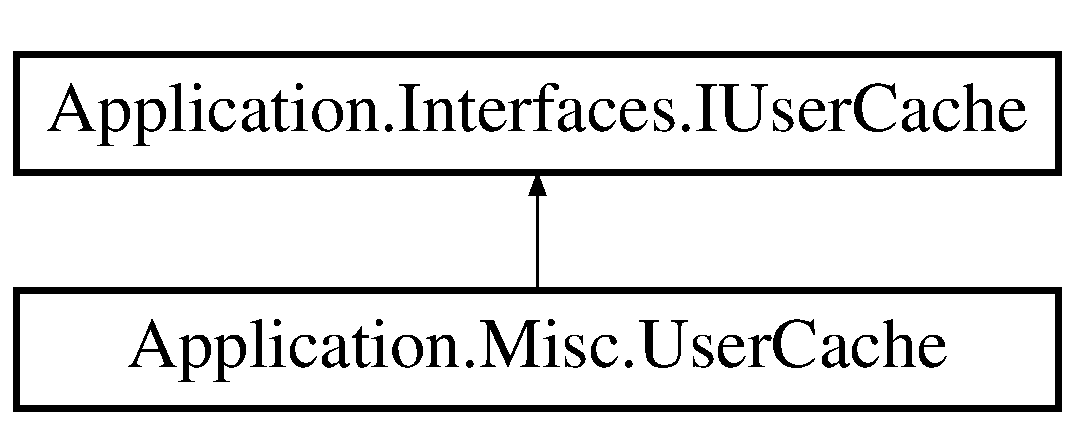
\includegraphics[height=2.000000cm]{interface_application_1_1_interfaces_1_1_i_user_cache}
\end{center}
\end{figure}
\subsection*{Public Member Functions}
\begin{DoxyCompactItemize}
\item 
void \mbox{\hyperlink{interface_application_1_1_interfaces_1_1_i_user_cache_a607deb5ebf1cfb0f237daf9981206d73}{Add\+Or\+Update}} (string username, string password)
\begin{DoxyCompactList}\small\item\em Adds a user to the cache with the default timeout of 20 minutes. \end{DoxyCompactList}\item 
void \mbox{\hyperlink{interface_application_1_1_interfaces_1_1_i_user_cache_aec631e3f0e466a067018b3196457056a}{Add\+Or\+Update}} (string username, string password, Date\+Time timeout)
\begin{DoxyCompactList}\small\item\em Adds a user to the cache with the timeout given in the paramater timeout. \end{DoxyCompactList}\item 
bool \mbox{\hyperlink{interface_application_1_1_interfaces_1_1_i_user_cache_a4978aad56d7292eafa02e8e7ad66f2c2}{Confirm}} (string username)
\begin{DoxyCompactList}\small\item\em Confirms that the user is currently in the cache. Does N\+OT refresh his timeout. \end{DoxyCompactList}\item 
bool \mbox{\hyperlink{interface_application_1_1_interfaces_1_1_i_user_cache_a3516a7abf1f40f9ddd10243cad03bb65}{Confirm\+And\+Refresh}} (string username, string password)
\begin{DoxyCompactList}\small\item\em Confirms that the user is currenty in the cache and if so refreshes the user\textquotesingle{}s timeout. The password must match. Returns true if user is found and refreshed, else false. \end{DoxyCompactList}\item 
bool \mbox{\hyperlink{interface_application_1_1_interfaces_1_1_i_user_cache_ac8ccbf20ac25069528e1e5117d5481ee}{Remove}} (string username, string password)
\begin{DoxyCompactList}\small\item\em Removes the user from the cache. Returns true if succesful. Else false. \end{DoxyCompactList}\end{DoxyCompactItemize}
\subsection*{Events}
\begin{DoxyCompactItemize}
\item 
Event\+Handler$<$ \mbox{\hyperlink{class_application_1_1_interfaces_1_1_timed_out_user_event_args}{Timed\+Out\+User\+Event\+Args}} $>$ \mbox{\hyperlink{interface_application_1_1_interfaces_1_1_i_user_cache_ae30035d1893d41c53cdd16627963a252}{Users\+Timed\+Out\+Event}}
\begin{DoxyCompactList}\small\item\em Users timeout event. Will contain a blocking collection of usernames that have been logged out. \end{DoxyCompactList}\end{DoxyCompactItemize}


\subsection{Member Function Documentation}
\mbox{\Hypertarget{interface_application_1_1_interfaces_1_1_i_user_cache_a607deb5ebf1cfb0f237daf9981206d73}\label{interface_application_1_1_interfaces_1_1_i_user_cache_a607deb5ebf1cfb0f237daf9981206d73}} 
\index{Application\+::\+Interfaces\+::\+I\+User\+Cache@{Application\+::\+Interfaces\+::\+I\+User\+Cache}!Add\+Or\+Update@{Add\+Or\+Update}}
\index{Add\+Or\+Update@{Add\+Or\+Update}!Application\+::\+Interfaces\+::\+I\+User\+Cache@{Application\+::\+Interfaces\+::\+I\+User\+Cache}}
\subsubsection{\texorpdfstring{Add\+Or\+Update()}{AddOrUpdate()}\hspace{0.1cm}{\footnotesize\ttfamily [1/2]}}
{\footnotesize\ttfamily void Application.\+Interfaces.\+I\+User\+Cache.\+Add\+Or\+Update (\begin{DoxyParamCaption}\item[{string}]{username,  }\item[{string}]{password }\end{DoxyParamCaption})}



Adds a user to the cache with the default timeout of 20 minutes. 


\begin{DoxyParams}{Parameters}
{\em username} & Username of user\\
\hline
{\em password} & password of user\\
\hline
\end{DoxyParams}
\begin{DoxyReturn}{Returns}

\end{DoxyReturn}


Implemented in \mbox{\hyperlink{class_application_1_1_misc_1_1_user_cache_ab56ecb52b9a7bc855729b439a5c5bb36}{Application.\+Misc.\+User\+Cache}}.

\mbox{\Hypertarget{interface_application_1_1_interfaces_1_1_i_user_cache_aec631e3f0e466a067018b3196457056a}\label{interface_application_1_1_interfaces_1_1_i_user_cache_aec631e3f0e466a067018b3196457056a}} 
\index{Application\+::\+Interfaces\+::\+I\+User\+Cache@{Application\+::\+Interfaces\+::\+I\+User\+Cache}!Add\+Or\+Update@{Add\+Or\+Update}}
\index{Add\+Or\+Update@{Add\+Or\+Update}!Application\+::\+Interfaces\+::\+I\+User\+Cache@{Application\+::\+Interfaces\+::\+I\+User\+Cache}}
\subsubsection{\texorpdfstring{Add\+Or\+Update()}{AddOrUpdate()}\hspace{0.1cm}{\footnotesize\ttfamily [2/2]}}
{\footnotesize\ttfamily void Application.\+Interfaces.\+I\+User\+Cache.\+Add\+Or\+Update (\begin{DoxyParamCaption}\item[{string}]{username,  }\item[{string}]{password,  }\item[{Date\+Time}]{timeout }\end{DoxyParamCaption})}



Adds a user to the cache with the timeout given in the paramater timeout. 


\begin{DoxyParams}{Parameters}
{\em username} & Username of user\\
\hline
{\em password} & password of user\\
\hline
{\em timeout} & \\
\hline
\end{DoxyParams}
\begin{DoxyReturn}{Returns}

\end{DoxyReturn}


Implemented in \mbox{\hyperlink{class_application_1_1_misc_1_1_user_cache_a7c8d6acdc76809a72a36db8ba8fdd8f8}{Application.\+Misc.\+User\+Cache}}.

\mbox{\Hypertarget{interface_application_1_1_interfaces_1_1_i_user_cache_a4978aad56d7292eafa02e8e7ad66f2c2}\label{interface_application_1_1_interfaces_1_1_i_user_cache_a4978aad56d7292eafa02e8e7ad66f2c2}} 
\index{Application\+::\+Interfaces\+::\+I\+User\+Cache@{Application\+::\+Interfaces\+::\+I\+User\+Cache}!Confirm@{Confirm}}
\index{Confirm@{Confirm}!Application\+::\+Interfaces\+::\+I\+User\+Cache@{Application\+::\+Interfaces\+::\+I\+User\+Cache}}
\subsubsection{\texorpdfstring{Confirm()}{Confirm()}}
{\footnotesize\ttfamily bool Application.\+Interfaces.\+I\+User\+Cache.\+Confirm (\begin{DoxyParamCaption}\item[{string}]{username }\end{DoxyParamCaption})}



Confirms that the user is currently in the cache. Does N\+OT refresh his timeout. 


\begin{DoxyParams}{Parameters}
{\em username} & \\
\hline
\end{DoxyParams}
\begin{DoxyReturn}{Returns}

\end{DoxyReturn}


Implemented in \mbox{\hyperlink{class_application_1_1_misc_1_1_user_cache_a77b10de2cba0f07aa9af6fd5ad53e2c6}{Application.\+Misc.\+User\+Cache}}.

\mbox{\Hypertarget{interface_application_1_1_interfaces_1_1_i_user_cache_a3516a7abf1f40f9ddd10243cad03bb65}\label{interface_application_1_1_interfaces_1_1_i_user_cache_a3516a7abf1f40f9ddd10243cad03bb65}} 
\index{Application\+::\+Interfaces\+::\+I\+User\+Cache@{Application\+::\+Interfaces\+::\+I\+User\+Cache}!Confirm\+And\+Refresh@{Confirm\+And\+Refresh}}
\index{Confirm\+And\+Refresh@{Confirm\+And\+Refresh}!Application\+::\+Interfaces\+::\+I\+User\+Cache@{Application\+::\+Interfaces\+::\+I\+User\+Cache}}
\subsubsection{\texorpdfstring{Confirm\+And\+Refresh()}{ConfirmAndRefresh()}}
{\footnotesize\ttfamily bool Application.\+Interfaces.\+I\+User\+Cache.\+Confirm\+And\+Refresh (\begin{DoxyParamCaption}\item[{string}]{username,  }\item[{string}]{password }\end{DoxyParamCaption})}



Confirms that the user is currenty in the cache and if so refreshes the user\textquotesingle{}s timeout. The password must match. Returns true if user is found and refreshed, else false. 


\begin{DoxyParams}{Parameters}
{\em username} & \\
\hline
{\em password} & \\
\hline
\end{DoxyParams}
\begin{DoxyReturn}{Returns}

\end{DoxyReturn}


Implemented in \mbox{\hyperlink{class_application_1_1_misc_1_1_user_cache_ad11a0422af31b1492098415d8e4aaad8}{Application.\+Misc.\+User\+Cache}}.

\mbox{\Hypertarget{interface_application_1_1_interfaces_1_1_i_user_cache_ac8ccbf20ac25069528e1e5117d5481ee}\label{interface_application_1_1_interfaces_1_1_i_user_cache_ac8ccbf20ac25069528e1e5117d5481ee}} 
\index{Application\+::\+Interfaces\+::\+I\+User\+Cache@{Application\+::\+Interfaces\+::\+I\+User\+Cache}!Remove@{Remove}}
\index{Remove@{Remove}!Application\+::\+Interfaces\+::\+I\+User\+Cache@{Application\+::\+Interfaces\+::\+I\+User\+Cache}}
\subsubsection{\texorpdfstring{Remove()}{Remove()}}
{\footnotesize\ttfamily bool Application.\+Interfaces.\+I\+User\+Cache.\+Remove (\begin{DoxyParamCaption}\item[{string}]{username,  }\item[{string}]{password }\end{DoxyParamCaption})}



Removes the user from the cache. Returns true if succesful. Else false. 


\begin{DoxyParams}{Parameters}
{\em username} & \\
\hline
{\em password} & \\
\hline
\end{DoxyParams}
\begin{DoxyReturn}{Returns}

\end{DoxyReturn}


Implemented in \mbox{\hyperlink{class_application_1_1_misc_1_1_user_cache_af685f56bf378e2bde07f7f6f933a8e0e}{Application.\+Misc.\+User\+Cache}}.



\subsection{Event Documentation}
\mbox{\Hypertarget{interface_application_1_1_interfaces_1_1_i_user_cache_ae30035d1893d41c53cdd16627963a252}\label{interface_application_1_1_interfaces_1_1_i_user_cache_ae30035d1893d41c53cdd16627963a252}} 
\index{Application\+::\+Interfaces\+::\+I\+User\+Cache@{Application\+::\+Interfaces\+::\+I\+User\+Cache}!Users\+Timed\+Out\+Event@{Users\+Timed\+Out\+Event}}
\index{Users\+Timed\+Out\+Event@{Users\+Timed\+Out\+Event}!Application\+::\+Interfaces\+::\+I\+User\+Cache@{Application\+::\+Interfaces\+::\+I\+User\+Cache}}
\subsubsection{\texorpdfstring{Users\+Timed\+Out\+Event}{UsersTimedOutEvent}}
{\footnotesize\ttfamily Event\+Handler$<$\mbox{\hyperlink{class_application_1_1_interfaces_1_1_timed_out_user_event_args}{Timed\+Out\+User\+Event\+Args}}$>$ Application.\+Interfaces.\+I\+User\+Cache.\+Users\+Timed\+Out\+Event}



Users timeout event. Will contain a blocking collection of usernames that have been logged out. 



The documentation for this interface was generated from the following file\+:\begin{DoxyCompactItemize}
\item 
Interfaces/\mbox{\hyperlink{_i_user_cache_8cs}{I\+User\+Cache.\+cs}}\end{DoxyCompactItemize}

\hypertarget{interface_application_1_1_interfaces_1_1_i_user_controller}{}\section{Application.\+Interfaces.\+I\+User\+Controller Interface Reference}
\label{interface_application_1_1_interfaces_1_1_i_user_controller}\index{Application.\+Interfaces.\+I\+User\+Controller@{Application.\+Interfaces.\+I\+User\+Controller}}
Inheritance diagram for Application.\+Interfaces.\+I\+User\+Controller\+:\begin{figure}[H]
\begin{center}
\leavevmode
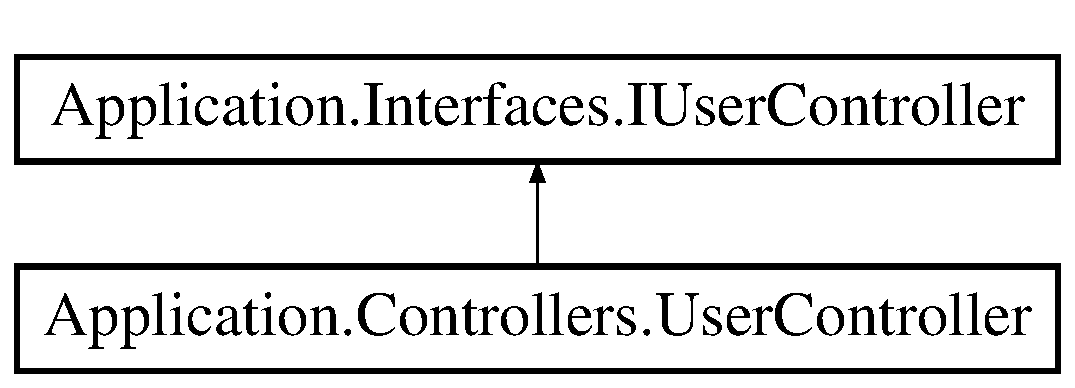
\includegraphics[height=2.000000cm]{interface_application_1_1_interfaces_1_1_i_user_controller}
\end{center}
\end{figure}
\subsection*{Public Member Functions}
\begin{DoxyCompactItemize}
\item 
I\+User \mbox{\hyperlink{interface_application_1_1_interfaces_1_1_i_user_controller_afdea9f68822192392d4b973e300f56af}{Get\+User}} (string username, string password)
\begin{DoxyCompactList}\small\item\em Returns the user with the given username and password. Null if not found \end{DoxyCompactList}\item 
I\+User \mbox{\hyperlink{interface_application_1_1_interfaces_1_1_i_user_controller_aca064ba3a4c3c2d0dd1339b8a4995e86}{Create\+User}} (I\+User user)
\begin{DoxyCompactList}\small\item\em Creates a new user to be stored in the database. Returns valid user upon succes. Otherwise null \end{DoxyCompactList}\item 
I\+User \mbox{\hyperlink{interface_application_1_1_interfaces_1_1_i_user_controller_a433f4021d60dafe735aff4d4b5536370}{Update\+User}} (string username, I\+User user)
\begin{DoxyCompactList}\small\item\em Updates the user as given by username and password. Will return null if unsuccesfull \end{DoxyCompactList}\end{DoxyCompactItemize}


\subsection{Member Function Documentation}
\mbox{\Hypertarget{interface_application_1_1_interfaces_1_1_i_user_controller_aca064ba3a4c3c2d0dd1339b8a4995e86}\label{interface_application_1_1_interfaces_1_1_i_user_controller_aca064ba3a4c3c2d0dd1339b8a4995e86}} 
\index{Application\+::\+Interfaces\+::\+I\+User\+Controller@{Application\+::\+Interfaces\+::\+I\+User\+Controller}!Create\+User@{Create\+User}}
\index{Create\+User@{Create\+User}!Application\+::\+Interfaces\+::\+I\+User\+Controller@{Application\+::\+Interfaces\+::\+I\+User\+Controller}}
\subsubsection{\texorpdfstring{Create\+User()}{CreateUser()}}
{\footnotesize\ttfamily I\+User Application.\+Interfaces.\+I\+User\+Controller.\+Create\+User (\begin{DoxyParamCaption}\item[{I\+User}]{user }\end{DoxyParamCaption})}



Creates a new user to be stored in the database. Returns valid user upon succes. Otherwise null 


\begin{DoxyParams}{Parameters}
{\em user} & User to be stored\\
\hline
\end{DoxyParams}
\begin{DoxyReturn}{Returns}

\end{DoxyReturn}


Implemented in \mbox{\hyperlink{class_application_1_1_controllers_1_1_user_controller_abf08955a5adc363fa137399a961a14fc}{Application.\+Controllers.\+User\+Controller}}.

\mbox{\Hypertarget{interface_application_1_1_interfaces_1_1_i_user_controller_afdea9f68822192392d4b973e300f56af}\label{interface_application_1_1_interfaces_1_1_i_user_controller_afdea9f68822192392d4b973e300f56af}} 
\index{Application\+::\+Interfaces\+::\+I\+User\+Controller@{Application\+::\+Interfaces\+::\+I\+User\+Controller}!Get\+User@{Get\+User}}
\index{Get\+User@{Get\+User}!Application\+::\+Interfaces\+::\+I\+User\+Controller@{Application\+::\+Interfaces\+::\+I\+User\+Controller}}
\subsubsection{\texorpdfstring{Get\+User()}{GetUser()}}
{\footnotesize\ttfamily I\+User Application.\+Interfaces.\+I\+User\+Controller.\+Get\+User (\begin{DoxyParamCaption}\item[{string}]{username,  }\item[{string}]{password }\end{DoxyParamCaption})}



Returns the user with the given username and password. Null if not found 


\begin{DoxyParams}{Parameters}
{\em username} & Username of requested user\\
\hline
{\em password} & Password of requested user\\
\hline
\end{DoxyParams}
\begin{DoxyReturn}{Returns}
User
\end{DoxyReturn}


Implemented in \mbox{\hyperlink{class_application_1_1_controllers_1_1_user_controller_adb2565915559692fae6a146d23d5fe01}{Application.\+Controllers.\+User\+Controller}}.

\mbox{\Hypertarget{interface_application_1_1_interfaces_1_1_i_user_controller_a433f4021d60dafe735aff4d4b5536370}\label{interface_application_1_1_interfaces_1_1_i_user_controller_a433f4021d60dafe735aff4d4b5536370}} 
\index{Application\+::\+Interfaces\+::\+I\+User\+Controller@{Application\+::\+Interfaces\+::\+I\+User\+Controller}!Update\+User@{Update\+User}}
\index{Update\+User@{Update\+User}!Application\+::\+Interfaces\+::\+I\+User\+Controller@{Application\+::\+Interfaces\+::\+I\+User\+Controller}}
\subsubsection{\texorpdfstring{Update\+User()}{UpdateUser()}}
{\footnotesize\ttfamily I\+User Application.\+Interfaces.\+I\+User\+Controller.\+Update\+User (\begin{DoxyParamCaption}\item[{string}]{username,  }\item[{I\+User}]{user }\end{DoxyParamCaption})}



Updates the user as given by username and password. Will return null if unsuccesfull 


\begin{DoxyParams}{Parameters}
{\em username} & Username of user to be updated\\
\hline
{\em user} & User object containing updated information\\
\hline
\end{DoxyParams}
\begin{DoxyReturn}{Returns}

\end{DoxyReturn}


Implemented in \mbox{\hyperlink{class_application_1_1_controllers_1_1_user_controller_af509b1d73f3a654edfb48dcc1f623ca8}{Application.\+Controllers.\+User\+Controller}}.



The documentation for this interface was generated from the following file\+:\begin{DoxyCompactItemize}
\item 
Interfaces/\mbox{\hyperlink{_i_user_controller_8cs}{I\+User\+Controller.\+cs}}\end{DoxyCompactItemize}

\hypertarget{class_application_1_1_controllers_1_1_lobby_controller}{}\section{Application.\+Controllers.\+Lobby\+Controller Class Reference}
\label{class_application_1_1_controllers_1_1_lobby_controller}\index{Application.\+Controllers.\+Lobby\+Controller@{Application.\+Controllers.\+Lobby\+Controller}}
Inheritance diagram for Application.\+Controllers.\+Lobby\+Controller\+:\begin{figure}[H]
\begin{center}
\leavevmode
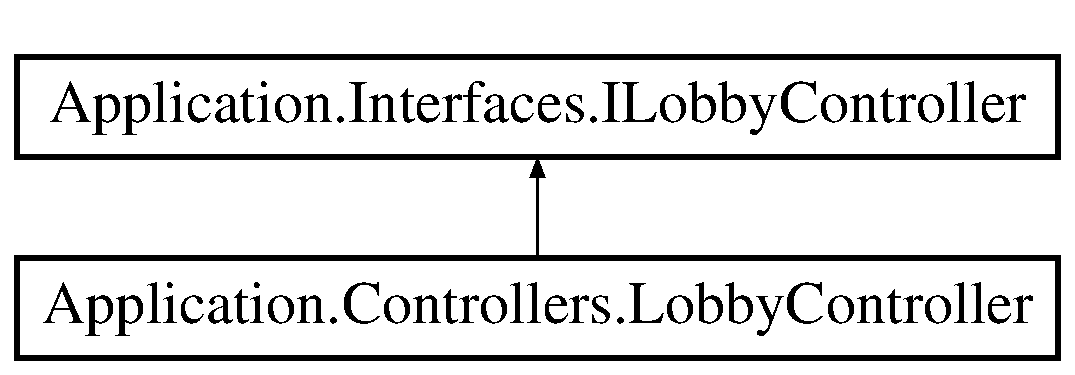
\includegraphics[height=2.000000cm]{class_application_1_1_controllers_1_1_lobby_controller}
\end{center}
\end{figure}
\subsection*{Public Member Functions}
\begin{DoxyCompactItemize}
\item 
\mbox{\hyperlink{class_application_1_1_controllers_1_1_lobby_controller_a9c832739ad9b40794194b0f142279b6e}{Lobby\+Controller}} (\mbox{\hyperlink{interface_application_1_1_interfaces_1_1_i_login_manager}{I\+Login\+Manager}} login\+Manager)
\item 
void \mbox{\hyperlink{class_application_1_1_controllers_1_1_lobby_controller_a3b6eb2c76ba2d3d96ddec5c56ab2abc2}{User\+Logged\+Out\+Event}} (object o, string username)
\item 
I\+Lobby \mbox{\hyperlink{class_application_1_1_controllers_1_1_lobby_controller_ad0684f9eace44951fcb75c805fb8574c}{Create\+Lobby}} (string lobby\+Id, string admin\+Username)
\begin{DoxyCompactList}\small\item\em Creates a new lobby and returns this \end{DoxyCompactList}\item 
I\+Lobby \mbox{\hyperlink{class_application_1_1_controllers_1_1_lobby_controller_ac081cab03ea49323b57c294ca95c6a09}{Join\+Lobby}} (string lobby\+Id, string username)
\item 
bool \mbox{\hyperlink{class_application_1_1_controllers_1_1_lobby_controller_aa075018713d8ac7fdf84cf6349e2f10d}{Leave\+Lobby}} (string lobby\+Id, string username)
\item 
I\+Lobby \mbox{\hyperlink{class_application_1_1_controllers_1_1_lobby_controller_a5ea797c6456dc8d40e16b87077a16693}{Get\+Lobby\+By\+Id}} (string lobby\+Id)
\item 
I\+Lobby \mbox{\hyperlink{class_application_1_1_controllers_1_1_lobby_controller_a415b61b5c78ba52619ac4d3606ecc32e}{Update\+Lobby}} (string admin\+Username, I\+Lobby lobby)
\begin{DoxyCompactList}\small\item\em Might not be useful. Is meant to update a lobby in scenarios where the admin user wishes to pass on this role to another user. \end{DoxyCompactList}\item 
I\+Collection$<$ string $>$ \mbox{\hyperlink{class_application_1_1_controllers_1_1_lobby_controller_a1aec115271209fc4ea59ed5f790d3011}{Get\+All\+Lobbies}} ()
\item 
async Task$<$ I\+Lobby $>$ \mbox{\hyperlink{class_application_1_1_controllers_1_1_lobby_controller_ac08d941f7da12f7791a691dbbdf0c1f3}{Create\+Lobby\+Async}} (string lobby\+Id, string admin\+Username)
\item 
async Task$<$ I\+Lobby $>$ \mbox{\hyperlink{class_application_1_1_controllers_1_1_lobby_controller_af9484a4c054717c0975175d93e45149c}{Join\+Lobby\+Async}} (string lobby\+Id, string username)
\item 
async Task$<$ bool $>$ \mbox{\hyperlink{class_application_1_1_controllers_1_1_lobby_controller_a7f0fb3932a42b76d5e4a9788aa0510e0}{Leave\+Lobby\+Async}} (string lobby\+Id, string username)
\item 
Task$<$ I\+Lobby $>$ \mbox{\hyperlink{class_application_1_1_controllers_1_1_lobby_controller_a2f30842e0480f28ddbe51ab420b35049}{Update\+Lobby\+Async}} (string admin\+Username, I\+Lobby lobby)
\item 
async Task$<$ I\+Collection$<$ string $>$ $>$ \mbox{\hyperlink{class_application_1_1_controllers_1_1_lobby_controller_a881adadc726a5daa68fe702439723630}{Get\+All\+Lobbies\+Async}} ()
\item 
async Task$<$ I\+Lobby $>$ \mbox{\hyperlink{class_application_1_1_controllers_1_1_lobby_controller_afe14da64961a1667fd7411484204c692}{Get\+Lobby\+By\+Id\+Async}} (string lobby\+Id)
\end{DoxyCompactItemize}
\subsection*{Properties}
\begin{DoxyCompactItemize}
\item 
I\+Read\+Only\+Dictionary$<$ string, I\+Lobby $>$ \mbox{\hyperlink{class_application_1_1_controllers_1_1_lobby_controller_adb1b5081f64dfe91e33d00b402632ec4}{Lobby\+Dictionary}}\hspace{0.3cm}{\ttfamily  \mbox{[}get\mbox{]}}
\begin{DoxyCompactList}\small\item\em Included for unit-\/testing purposes. \end{DoxyCompactList}\end{DoxyCompactItemize}


\subsection{Constructor \& Destructor Documentation}
\mbox{\Hypertarget{class_application_1_1_controllers_1_1_lobby_controller_a9c832739ad9b40794194b0f142279b6e}\label{class_application_1_1_controllers_1_1_lobby_controller_a9c832739ad9b40794194b0f142279b6e}} 
\index{Application\+::\+Controllers\+::\+Lobby\+Controller@{Application\+::\+Controllers\+::\+Lobby\+Controller}!Lobby\+Controller@{Lobby\+Controller}}
\index{Lobby\+Controller@{Lobby\+Controller}!Application\+::\+Controllers\+::\+Lobby\+Controller@{Application\+::\+Controllers\+::\+Lobby\+Controller}}
\subsubsection{\texorpdfstring{Lobby\+Controller()}{LobbyController()}}
{\footnotesize\ttfamily Application.\+Controllers.\+Lobby\+Controller.\+Lobby\+Controller (\begin{DoxyParamCaption}\item[{\mbox{\hyperlink{interface_application_1_1_interfaces_1_1_i_login_manager}{I\+Login\+Manager}}}]{login\+Manager }\end{DoxyParamCaption})}



\subsection{Member Function Documentation}
\mbox{\Hypertarget{class_application_1_1_controllers_1_1_lobby_controller_ad0684f9eace44951fcb75c805fb8574c}\label{class_application_1_1_controllers_1_1_lobby_controller_ad0684f9eace44951fcb75c805fb8574c}} 
\index{Application\+::\+Controllers\+::\+Lobby\+Controller@{Application\+::\+Controllers\+::\+Lobby\+Controller}!Create\+Lobby@{Create\+Lobby}}
\index{Create\+Lobby@{Create\+Lobby}!Application\+::\+Controllers\+::\+Lobby\+Controller@{Application\+::\+Controllers\+::\+Lobby\+Controller}}
\subsubsection{\texorpdfstring{Create\+Lobby()}{CreateLobby()}}
{\footnotesize\ttfamily I\+Lobby Application.\+Controllers.\+Lobby\+Controller.\+Create\+Lobby (\begin{DoxyParamCaption}\item[{string}]{lobby\+Id,  }\item[{string}]{admin\+Username }\end{DoxyParamCaption})}



Creates a new lobby and returns this 


\begin{DoxyParams}{Parameters}
{\em lobby\+Id} & The id of the lobby to create\\
\hline
{\em admin\+Username} & The username to be assigned as admin of the lobby\\
\hline
\end{DoxyParams}
\begin{DoxyReturn}{Returns}
Returns a new lobby with the passed information if the lobby id isen\textquotesingle{}t taken and if the user is not currently attached to another lobby. Else null.
\end{DoxyReturn}


Implements \mbox{\hyperlink{interface_application_1_1_interfaces_1_1_i_lobby_controller_abefe3510b20e3db41c4d8062f8cdc2bc}{Application.\+Interfaces.\+I\+Lobby\+Controller}}.

\mbox{\Hypertarget{class_application_1_1_controllers_1_1_lobby_controller_ac08d941f7da12f7791a691dbbdf0c1f3}\label{class_application_1_1_controllers_1_1_lobby_controller_ac08d941f7da12f7791a691dbbdf0c1f3}} 
\index{Application\+::\+Controllers\+::\+Lobby\+Controller@{Application\+::\+Controllers\+::\+Lobby\+Controller}!Create\+Lobby\+Async@{Create\+Lobby\+Async}}
\index{Create\+Lobby\+Async@{Create\+Lobby\+Async}!Application\+::\+Controllers\+::\+Lobby\+Controller@{Application\+::\+Controllers\+::\+Lobby\+Controller}}
\subsubsection{\texorpdfstring{Create\+Lobby\+Async()}{CreateLobbyAsync()}}
{\footnotesize\ttfamily async Task$<$I\+Lobby$>$ Application.\+Controllers.\+Lobby\+Controller.\+Create\+Lobby\+Async (\begin{DoxyParamCaption}\item[{string}]{lobby\+Id,  }\item[{string}]{admin\+Username }\end{DoxyParamCaption})}



Implements \mbox{\hyperlink{interface_application_1_1_interfaces_1_1_i_lobby_controller_ae507a1d23088662b8c37692bbb93040e}{Application.\+Interfaces.\+I\+Lobby\+Controller}}.

\mbox{\Hypertarget{class_application_1_1_controllers_1_1_lobby_controller_a1aec115271209fc4ea59ed5f790d3011}\label{class_application_1_1_controllers_1_1_lobby_controller_a1aec115271209fc4ea59ed5f790d3011}} 
\index{Application\+::\+Controllers\+::\+Lobby\+Controller@{Application\+::\+Controllers\+::\+Lobby\+Controller}!Get\+All\+Lobbies@{Get\+All\+Lobbies}}
\index{Get\+All\+Lobbies@{Get\+All\+Lobbies}!Application\+::\+Controllers\+::\+Lobby\+Controller@{Application\+::\+Controllers\+::\+Lobby\+Controller}}
\subsubsection{\texorpdfstring{Get\+All\+Lobbies()}{GetAllLobbies()}}
{\footnotesize\ttfamily I\+Collection$<$string$>$ Application.\+Controllers.\+Lobby\+Controller.\+Get\+All\+Lobbies (\begin{DoxyParamCaption}{ }\end{DoxyParamCaption})}



Implements \mbox{\hyperlink{interface_application_1_1_interfaces_1_1_i_lobby_controller_a2e1d8f72361ee48e956fb473ceabadf4}{Application.\+Interfaces.\+I\+Lobby\+Controller}}.

\mbox{\Hypertarget{class_application_1_1_controllers_1_1_lobby_controller_a881adadc726a5daa68fe702439723630}\label{class_application_1_1_controllers_1_1_lobby_controller_a881adadc726a5daa68fe702439723630}} 
\index{Application\+::\+Controllers\+::\+Lobby\+Controller@{Application\+::\+Controllers\+::\+Lobby\+Controller}!Get\+All\+Lobbies\+Async@{Get\+All\+Lobbies\+Async}}
\index{Get\+All\+Lobbies\+Async@{Get\+All\+Lobbies\+Async}!Application\+::\+Controllers\+::\+Lobby\+Controller@{Application\+::\+Controllers\+::\+Lobby\+Controller}}
\subsubsection{\texorpdfstring{Get\+All\+Lobbies\+Async()}{GetAllLobbiesAsync()}}
{\footnotesize\ttfamily async Task$<$I\+Collection$<$string$>$ $>$ Application.\+Controllers.\+Lobby\+Controller.\+Get\+All\+Lobbies\+Async (\begin{DoxyParamCaption}{ }\end{DoxyParamCaption})}



Implements \mbox{\hyperlink{interface_application_1_1_interfaces_1_1_i_lobby_controller_acf938121367844d623fa4127cf643e50}{Application.\+Interfaces.\+I\+Lobby\+Controller}}.

\mbox{\Hypertarget{class_application_1_1_controllers_1_1_lobby_controller_a5ea797c6456dc8d40e16b87077a16693}\label{class_application_1_1_controllers_1_1_lobby_controller_a5ea797c6456dc8d40e16b87077a16693}} 
\index{Application\+::\+Controllers\+::\+Lobby\+Controller@{Application\+::\+Controllers\+::\+Lobby\+Controller}!Get\+Lobby\+By\+Id@{Get\+Lobby\+By\+Id}}
\index{Get\+Lobby\+By\+Id@{Get\+Lobby\+By\+Id}!Application\+::\+Controllers\+::\+Lobby\+Controller@{Application\+::\+Controllers\+::\+Lobby\+Controller}}
\subsubsection{\texorpdfstring{Get\+Lobby\+By\+Id()}{GetLobbyById()}}
{\footnotesize\ttfamily I\+Lobby Application.\+Controllers.\+Lobby\+Controller.\+Get\+Lobby\+By\+Id (\begin{DoxyParamCaption}\item[{string}]{lobby\+Id }\end{DoxyParamCaption})}



Implements \mbox{\hyperlink{interface_application_1_1_interfaces_1_1_i_lobby_controller_aaa584fec6fc0e1e0690aa81e7fde3af2}{Application.\+Interfaces.\+I\+Lobby\+Controller}}.

\mbox{\Hypertarget{class_application_1_1_controllers_1_1_lobby_controller_afe14da64961a1667fd7411484204c692}\label{class_application_1_1_controllers_1_1_lobby_controller_afe14da64961a1667fd7411484204c692}} 
\index{Application\+::\+Controllers\+::\+Lobby\+Controller@{Application\+::\+Controllers\+::\+Lobby\+Controller}!Get\+Lobby\+By\+Id\+Async@{Get\+Lobby\+By\+Id\+Async}}
\index{Get\+Lobby\+By\+Id\+Async@{Get\+Lobby\+By\+Id\+Async}!Application\+::\+Controllers\+::\+Lobby\+Controller@{Application\+::\+Controllers\+::\+Lobby\+Controller}}
\subsubsection{\texorpdfstring{Get\+Lobby\+By\+Id\+Async()}{GetLobbyByIdAsync()}}
{\footnotesize\ttfamily async Task$<$I\+Lobby$>$ Application.\+Controllers.\+Lobby\+Controller.\+Get\+Lobby\+By\+Id\+Async (\begin{DoxyParamCaption}\item[{string}]{lobby\+Id }\end{DoxyParamCaption})}



Implements \mbox{\hyperlink{interface_application_1_1_interfaces_1_1_i_lobby_controller_abe3ce90e900391a0c4ffa25195800ab2}{Application.\+Interfaces.\+I\+Lobby\+Controller}}.

\mbox{\Hypertarget{class_application_1_1_controllers_1_1_lobby_controller_ac081cab03ea49323b57c294ca95c6a09}\label{class_application_1_1_controllers_1_1_lobby_controller_ac081cab03ea49323b57c294ca95c6a09}} 
\index{Application\+::\+Controllers\+::\+Lobby\+Controller@{Application\+::\+Controllers\+::\+Lobby\+Controller}!Join\+Lobby@{Join\+Lobby}}
\index{Join\+Lobby@{Join\+Lobby}!Application\+::\+Controllers\+::\+Lobby\+Controller@{Application\+::\+Controllers\+::\+Lobby\+Controller}}
\subsubsection{\texorpdfstring{Join\+Lobby()}{JoinLobby()}}
{\footnotesize\ttfamily I\+Lobby Application.\+Controllers.\+Lobby\+Controller.\+Join\+Lobby (\begin{DoxyParamCaption}\item[{string}]{lobby\+Id,  }\item[{string}]{username }\end{DoxyParamCaption})}



Implements \mbox{\hyperlink{interface_application_1_1_interfaces_1_1_i_lobby_controller_a17c37ec6dbb98ab07deb4e4f9800a68e}{Application.\+Interfaces.\+I\+Lobby\+Controller}}.

\mbox{\Hypertarget{class_application_1_1_controllers_1_1_lobby_controller_af9484a4c054717c0975175d93e45149c}\label{class_application_1_1_controllers_1_1_lobby_controller_af9484a4c054717c0975175d93e45149c}} 
\index{Application\+::\+Controllers\+::\+Lobby\+Controller@{Application\+::\+Controllers\+::\+Lobby\+Controller}!Join\+Lobby\+Async@{Join\+Lobby\+Async}}
\index{Join\+Lobby\+Async@{Join\+Lobby\+Async}!Application\+::\+Controllers\+::\+Lobby\+Controller@{Application\+::\+Controllers\+::\+Lobby\+Controller}}
\subsubsection{\texorpdfstring{Join\+Lobby\+Async()}{JoinLobbyAsync()}}
{\footnotesize\ttfamily async Task$<$I\+Lobby$>$ Application.\+Controllers.\+Lobby\+Controller.\+Join\+Lobby\+Async (\begin{DoxyParamCaption}\item[{string}]{lobby\+Id,  }\item[{string}]{username }\end{DoxyParamCaption})}



Implements \mbox{\hyperlink{interface_application_1_1_interfaces_1_1_i_lobby_controller_aba87a2245b2c274cf977aeaf193eef73}{Application.\+Interfaces.\+I\+Lobby\+Controller}}.

\mbox{\Hypertarget{class_application_1_1_controllers_1_1_lobby_controller_aa075018713d8ac7fdf84cf6349e2f10d}\label{class_application_1_1_controllers_1_1_lobby_controller_aa075018713d8ac7fdf84cf6349e2f10d}} 
\index{Application\+::\+Controllers\+::\+Lobby\+Controller@{Application\+::\+Controllers\+::\+Lobby\+Controller}!Leave\+Lobby@{Leave\+Lobby}}
\index{Leave\+Lobby@{Leave\+Lobby}!Application\+::\+Controllers\+::\+Lobby\+Controller@{Application\+::\+Controllers\+::\+Lobby\+Controller}}
\subsubsection{\texorpdfstring{Leave\+Lobby()}{LeaveLobby()}}
{\footnotesize\ttfamily bool Application.\+Controllers.\+Lobby\+Controller.\+Leave\+Lobby (\begin{DoxyParamCaption}\item[{string}]{lobby\+Id,  }\item[{string}]{username }\end{DoxyParamCaption})}



Implements \mbox{\hyperlink{interface_application_1_1_interfaces_1_1_i_lobby_controller_ad95e5c656813094f7abec7b81ea568e1}{Application.\+Interfaces.\+I\+Lobby\+Controller}}.

\mbox{\Hypertarget{class_application_1_1_controllers_1_1_lobby_controller_a7f0fb3932a42b76d5e4a9788aa0510e0}\label{class_application_1_1_controllers_1_1_lobby_controller_a7f0fb3932a42b76d5e4a9788aa0510e0}} 
\index{Application\+::\+Controllers\+::\+Lobby\+Controller@{Application\+::\+Controllers\+::\+Lobby\+Controller}!Leave\+Lobby\+Async@{Leave\+Lobby\+Async}}
\index{Leave\+Lobby\+Async@{Leave\+Lobby\+Async}!Application\+::\+Controllers\+::\+Lobby\+Controller@{Application\+::\+Controllers\+::\+Lobby\+Controller}}
\subsubsection{\texorpdfstring{Leave\+Lobby\+Async()}{LeaveLobbyAsync()}}
{\footnotesize\ttfamily async Task$<$bool$>$ Application.\+Controllers.\+Lobby\+Controller.\+Leave\+Lobby\+Async (\begin{DoxyParamCaption}\item[{string}]{lobby\+Id,  }\item[{string}]{username }\end{DoxyParamCaption})}



Implements \mbox{\hyperlink{interface_application_1_1_interfaces_1_1_i_lobby_controller_a46975c7e9219d5324f786542a23d9e7e}{Application.\+Interfaces.\+I\+Lobby\+Controller}}.

\mbox{\Hypertarget{class_application_1_1_controllers_1_1_lobby_controller_a415b61b5c78ba52619ac4d3606ecc32e}\label{class_application_1_1_controllers_1_1_lobby_controller_a415b61b5c78ba52619ac4d3606ecc32e}} 
\index{Application\+::\+Controllers\+::\+Lobby\+Controller@{Application\+::\+Controllers\+::\+Lobby\+Controller}!Update\+Lobby@{Update\+Lobby}}
\index{Update\+Lobby@{Update\+Lobby}!Application\+::\+Controllers\+::\+Lobby\+Controller@{Application\+::\+Controllers\+::\+Lobby\+Controller}}
\subsubsection{\texorpdfstring{Update\+Lobby()}{UpdateLobby()}}
{\footnotesize\ttfamily I\+Lobby Application.\+Controllers.\+Lobby\+Controller.\+Update\+Lobby (\begin{DoxyParamCaption}\item[{string}]{admin\+Username,  }\item[{I\+Lobby}]{lobby }\end{DoxyParamCaption})}



Might not be useful. Is meant to update a lobby in scenarios where the admin user wishes to pass on this role to another user. 


\begin{DoxyParams}{Parameters}
{\em admin\+Username} & Username of the current admin of the passed \mbox{\hyperlink{}{I\+Lobby}} lobby\\
\hline
{\em lobby} & The lobby to update\\
\hline
\end{DoxyParams}
\begin{DoxyReturn}{Returns}
The updated lobby upon succes. Else null.
\end{DoxyReturn}


Implements \mbox{\hyperlink{interface_application_1_1_interfaces_1_1_i_lobby_controller_a4d0618e880423f15785360453bf90f90}{Application.\+Interfaces.\+I\+Lobby\+Controller}}.

\mbox{\Hypertarget{class_application_1_1_controllers_1_1_lobby_controller_a2f30842e0480f28ddbe51ab420b35049}\label{class_application_1_1_controllers_1_1_lobby_controller_a2f30842e0480f28ddbe51ab420b35049}} 
\index{Application\+::\+Controllers\+::\+Lobby\+Controller@{Application\+::\+Controllers\+::\+Lobby\+Controller}!Update\+Lobby\+Async@{Update\+Lobby\+Async}}
\index{Update\+Lobby\+Async@{Update\+Lobby\+Async}!Application\+::\+Controllers\+::\+Lobby\+Controller@{Application\+::\+Controllers\+::\+Lobby\+Controller}}
\subsubsection{\texorpdfstring{Update\+Lobby\+Async()}{UpdateLobbyAsync()}}
{\footnotesize\ttfamily Task$<$I\+Lobby$>$ Application.\+Controllers.\+Lobby\+Controller.\+Update\+Lobby\+Async (\begin{DoxyParamCaption}\item[{string}]{admin\+Username,  }\item[{I\+Lobby}]{lobby }\end{DoxyParamCaption})}



Implements \mbox{\hyperlink{interface_application_1_1_interfaces_1_1_i_lobby_controller_a40457a8fb8d6801a8e42f1e75f9d3480}{Application.\+Interfaces.\+I\+Lobby\+Controller}}.

\mbox{\Hypertarget{class_application_1_1_controllers_1_1_lobby_controller_a3b6eb2c76ba2d3d96ddec5c56ab2abc2}\label{class_application_1_1_controllers_1_1_lobby_controller_a3b6eb2c76ba2d3d96ddec5c56ab2abc2}} 
\index{Application\+::\+Controllers\+::\+Lobby\+Controller@{Application\+::\+Controllers\+::\+Lobby\+Controller}!User\+Logged\+Out\+Event@{User\+Logged\+Out\+Event}}
\index{User\+Logged\+Out\+Event@{User\+Logged\+Out\+Event}!Application\+::\+Controllers\+::\+Lobby\+Controller@{Application\+::\+Controllers\+::\+Lobby\+Controller}}
\subsubsection{\texorpdfstring{User\+Logged\+Out\+Event()}{UserLoggedOutEvent()}}
{\footnotesize\ttfamily void Application.\+Controllers.\+Lobby\+Controller.\+User\+Logged\+Out\+Event (\begin{DoxyParamCaption}\item[{object}]{o,  }\item[{string}]{username }\end{DoxyParamCaption})}



\subsection{Property Documentation}
\mbox{\Hypertarget{class_application_1_1_controllers_1_1_lobby_controller_adb1b5081f64dfe91e33d00b402632ec4}\label{class_application_1_1_controllers_1_1_lobby_controller_adb1b5081f64dfe91e33d00b402632ec4}} 
\index{Application\+::\+Controllers\+::\+Lobby\+Controller@{Application\+::\+Controllers\+::\+Lobby\+Controller}!Lobby\+Dictionary@{Lobby\+Dictionary}}
\index{Lobby\+Dictionary@{Lobby\+Dictionary}!Application\+::\+Controllers\+::\+Lobby\+Controller@{Application\+::\+Controllers\+::\+Lobby\+Controller}}
\subsubsection{\texorpdfstring{Lobby\+Dictionary}{LobbyDictionary}}
{\footnotesize\ttfamily I\+Read\+Only\+Dictionary$<$string, I\+Lobby$>$ Application.\+Controllers.\+Lobby\+Controller.\+Lobby\+Dictionary\hspace{0.3cm}{\ttfamily [get]}}



Included for unit-\/testing purposes. 



The documentation for this class was generated from the following file\+:\begin{DoxyCompactItemize}
\item 
Controllers/\mbox{\hyperlink{_lobby_controller_8cs}{Lobby\+Controller.\+cs}}\end{DoxyCompactItemize}

\hypertarget{class_application_1_1_misc_1_1_lobby_pool}{}\section{Application.\+Misc.\+Lobby\+Pool Class Reference}
\label{class_application_1_1_misc_1_1_lobby_pool}\index{Application.\+Misc.\+Lobby\+Pool@{Application.\+Misc.\+Lobby\+Pool}}
Inheritance diagram for Application.\+Misc.\+Lobby\+Pool\+:\begin{figure}[H]
\begin{center}
\leavevmode
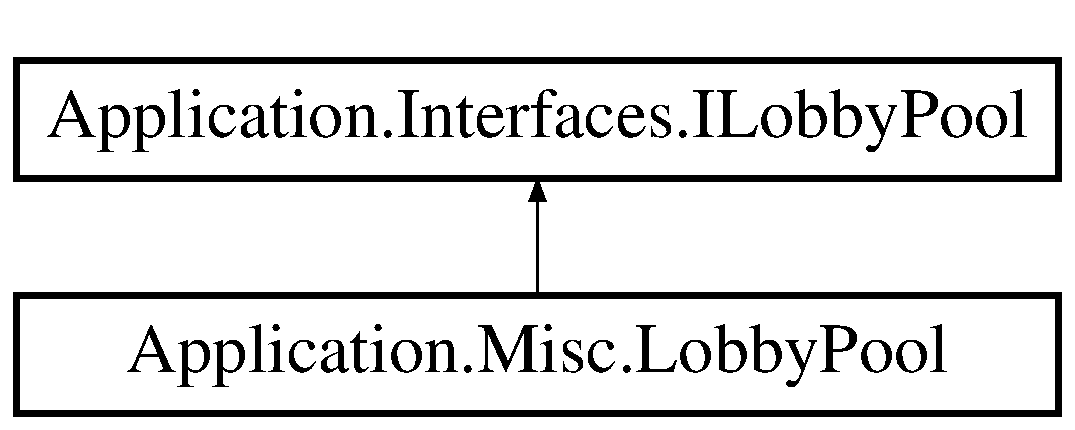
\includegraphics[height=2.000000cm]{class_application_1_1_misc_1_1_lobby_pool}
\end{center}
\end{figure}
\subsection*{Public Member Functions}
\begin{DoxyCompactItemize}
\item 
\mbox{\hyperlink{class_application_1_1_misc_1_1_lobby_pool_adefb9ad44d5c53d09f31a79ff5a96e89}{Lobby\+Pool}} ()
\item 
bool \mbox{\hyperlink{class_application_1_1_misc_1_1_lobby_pool_a442eb666b16bc75025732413f38b0846}{Add\+Lobby}} (I\+Lobby lobby)
\item 
I\+Lobby \mbox{\hyperlink{class_application_1_1_misc_1_1_lobby_pool_a61b2a303bd4bc1e72e31b3ee3d1e06d5}{Get\+Lobby}} (string lobby\+Id)
\item 
bool \mbox{\hyperlink{class_application_1_1_misc_1_1_lobby_pool_a747cfa417f8932fa8b006b6662c45099}{Release\+Lobby}} (string lobby\+Id)
\item 
I\+Enumerable$<$ I\+Lobby $>$ \mbox{\hyperlink{class_application_1_1_misc_1_1_lobby_pool_a3d1c9e496386713ad5d8ede307e6c28c}{Find}} (Func$<$ I\+Lobby, bool $>$ expression)
\item 
I\+Lobby \mbox{\hyperlink{class_application_1_1_misc_1_1_lobby_pool_a5676f006bc10c46224c1b3bb266702a3}{First\+Or\+Default}} (Func$<$ I\+Lobby, bool $>$ func)
\item 
bool \mbox{\hyperlink{class_application_1_1_misc_1_1_lobby_pool_af9f3a5b65c1a948fa63796a907c1684d}{Contains}} (string lobby\+Id)
\end{DoxyCompactItemize}
\subsection*{Public Attributes}
\begin{DoxyCompactItemize}
\item 
I\+Collection$<$ string $>$ \mbox{\hyperlink{class_application_1_1_misc_1_1_lobby_pool_a458073f24e69b53446da0a03050664e1}{Lobbies\+Collection}} =$>$ \+\_\+lobby\+Dictionary\+Pool.\+Keys.\+To\+List()
\item 
I\+Read\+Only\+Dictionary$<$ string, I\+Lobby $>$ \mbox{\hyperlink{class_application_1_1_misc_1_1_lobby_pool_a807b21ba18c87a433c8d9ff1fc5c00f1}{Lobby\+Dictionary}} =$>$ \+\_\+lobby\+Dictionary\+Pool
\end{DoxyCompactItemize}
\subsection*{Additional Inherited Members}


\subsection{Constructor \& Destructor Documentation}
\mbox{\Hypertarget{class_application_1_1_misc_1_1_lobby_pool_adefb9ad44d5c53d09f31a79ff5a96e89}\label{class_application_1_1_misc_1_1_lobby_pool_adefb9ad44d5c53d09f31a79ff5a96e89}} 
\index{Application\+::\+Misc\+::\+Lobby\+Pool@{Application\+::\+Misc\+::\+Lobby\+Pool}!Lobby\+Pool@{Lobby\+Pool}}
\index{Lobby\+Pool@{Lobby\+Pool}!Application\+::\+Misc\+::\+Lobby\+Pool@{Application\+::\+Misc\+::\+Lobby\+Pool}}
\subsubsection{\texorpdfstring{Lobby\+Pool()}{LobbyPool()}}
{\footnotesize\ttfamily Application.\+Misc.\+Lobby\+Pool.\+Lobby\+Pool (\begin{DoxyParamCaption}{ }\end{DoxyParamCaption})}



\subsection{Member Function Documentation}
\mbox{\Hypertarget{class_application_1_1_misc_1_1_lobby_pool_a442eb666b16bc75025732413f38b0846}\label{class_application_1_1_misc_1_1_lobby_pool_a442eb666b16bc75025732413f38b0846}} 
\index{Application\+::\+Misc\+::\+Lobby\+Pool@{Application\+::\+Misc\+::\+Lobby\+Pool}!Add\+Lobby@{Add\+Lobby}}
\index{Add\+Lobby@{Add\+Lobby}!Application\+::\+Misc\+::\+Lobby\+Pool@{Application\+::\+Misc\+::\+Lobby\+Pool}}
\subsubsection{\texorpdfstring{Add\+Lobby()}{AddLobby()}}
{\footnotesize\ttfamily bool Application.\+Misc.\+Lobby\+Pool.\+Add\+Lobby (\begin{DoxyParamCaption}\item[{I\+Lobby}]{lobby }\end{DoxyParamCaption})}



Implements \mbox{\hyperlink{interface_application_1_1_interfaces_1_1_i_lobby_pool_a2aa933d501630b665f67c68e39012a4c}{Application.\+Interfaces.\+I\+Lobby\+Pool}}.

\mbox{\Hypertarget{class_application_1_1_misc_1_1_lobby_pool_af9f3a5b65c1a948fa63796a907c1684d}\label{class_application_1_1_misc_1_1_lobby_pool_af9f3a5b65c1a948fa63796a907c1684d}} 
\index{Application\+::\+Misc\+::\+Lobby\+Pool@{Application\+::\+Misc\+::\+Lobby\+Pool}!Contains@{Contains}}
\index{Contains@{Contains}!Application\+::\+Misc\+::\+Lobby\+Pool@{Application\+::\+Misc\+::\+Lobby\+Pool}}
\subsubsection{\texorpdfstring{Contains()}{Contains()}}
{\footnotesize\ttfamily bool Application.\+Misc.\+Lobby\+Pool.\+Contains (\begin{DoxyParamCaption}\item[{string}]{lobby\+Id }\end{DoxyParamCaption})}



Implements \mbox{\hyperlink{interface_application_1_1_interfaces_1_1_i_lobby_pool_a9a09df8415ae760c99d5a6bcd1ac91f9}{Application.\+Interfaces.\+I\+Lobby\+Pool}}.

\mbox{\Hypertarget{class_application_1_1_misc_1_1_lobby_pool_a3d1c9e496386713ad5d8ede307e6c28c}\label{class_application_1_1_misc_1_1_lobby_pool_a3d1c9e496386713ad5d8ede307e6c28c}} 
\index{Application\+::\+Misc\+::\+Lobby\+Pool@{Application\+::\+Misc\+::\+Lobby\+Pool}!Find@{Find}}
\index{Find@{Find}!Application\+::\+Misc\+::\+Lobby\+Pool@{Application\+::\+Misc\+::\+Lobby\+Pool}}
\subsubsection{\texorpdfstring{Find()}{Find()}}
{\footnotesize\ttfamily I\+Enumerable$<$I\+Lobby$>$ Application.\+Misc.\+Lobby\+Pool.\+Find (\begin{DoxyParamCaption}\item[{Func$<$ I\+Lobby, bool $>$}]{expression }\end{DoxyParamCaption})}



Implements \mbox{\hyperlink{interface_application_1_1_interfaces_1_1_i_lobby_pool_ac64adf71b4ab967725dec520bab627c3}{Application.\+Interfaces.\+I\+Lobby\+Pool}}.

\mbox{\Hypertarget{class_application_1_1_misc_1_1_lobby_pool_a5676f006bc10c46224c1b3bb266702a3}\label{class_application_1_1_misc_1_1_lobby_pool_a5676f006bc10c46224c1b3bb266702a3}} 
\index{Application\+::\+Misc\+::\+Lobby\+Pool@{Application\+::\+Misc\+::\+Lobby\+Pool}!First\+Or\+Default@{First\+Or\+Default}}
\index{First\+Or\+Default@{First\+Or\+Default}!Application\+::\+Misc\+::\+Lobby\+Pool@{Application\+::\+Misc\+::\+Lobby\+Pool}}
\subsubsection{\texorpdfstring{First\+Or\+Default()}{FirstOrDefault()}}
{\footnotesize\ttfamily I\+Lobby Application.\+Misc.\+Lobby\+Pool.\+First\+Or\+Default (\begin{DoxyParamCaption}\item[{Func$<$ I\+Lobby, bool $>$}]{func }\end{DoxyParamCaption})}



Implements \mbox{\hyperlink{interface_application_1_1_interfaces_1_1_i_lobby_pool_aa518351cc8b58ef5997f7ecef19633bb}{Application.\+Interfaces.\+I\+Lobby\+Pool}}.

\mbox{\Hypertarget{class_application_1_1_misc_1_1_lobby_pool_a61b2a303bd4bc1e72e31b3ee3d1e06d5}\label{class_application_1_1_misc_1_1_lobby_pool_a61b2a303bd4bc1e72e31b3ee3d1e06d5}} 
\index{Application\+::\+Misc\+::\+Lobby\+Pool@{Application\+::\+Misc\+::\+Lobby\+Pool}!Get\+Lobby@{Get\+Lobby}}
\index{Get\+Lobby@{Get\+Lobby}!Application\+::\+Misc\+::\+Lobby\+Pool@{Application\+::\+Misc\+::\+Lobby\+Pool}}
\subsubsection{\texorpdfstring{Get\+Lobby()}{GetLobby()}}
{\footnotesize\ttfamily I\+Lobby Application.\+Misc.\+Lobby\+Pool.\+Get\+Lobby (\begin{DoxyParamCaption}\item[{string}]{lobby\+Id }\end{DoxyParamCaption})}



Implements \mbox{\hyperlink{interface_application_1_1_interfaces_1_1_i_lobby_pool_a044d19c090cbd70a17de4b487fd6d613}{Application.\+Interfaces.\+I\+Lobby\+Pool}}.

\mbox{\Hypertarget{class_application_1_1_misc_1_1_lobby_pool_a747cfa417f8932fa8b006b6662c45099}\label{class_application_1_1_misc_1_1_lobby_pool_a747cfa417f8932fa8b006b6662c45099}} 
\index{Application\+::\+Misc\+::\+Lobby\+Pool@{Application\+::\+Misc\+::\+Lobby\+Pool}!Release\+Lobby@{Release\+Lobby}}
\index{Release\+Lobby@{Release\+Lobby}!Application\+::\+Misc\+::\+Lobby\+Pool@{Application\+::\+Misc\+::\+Lobby\+Pool}}
\subsubsection{\texorpdfstring{Release\+Lobby()}{ReleaseLobby()}}
{\footnotesize\ttfamily bool Application.\+Misc.\+Lobby\+Pool.\+Release\+Lobby (\begin{DoxyParamCaption}\item[{string}]{lobby\+Id }\end{DoxyParamCaption})}



Implements \mbox{\hyperlink{interface_application_1_1_interfaces_1_1_i_lobby_pool_a61058848af185e20841421e7f52e8b94}{Application.\+Interfaces.\+I\+Lobby\+Pool}}.



\subsection{Member Data Documentation}
\mbox{\Hypertarget{class_application_1_1_misc_1_1_lobby_pool_a458073f24e69b53446da0a03050664e1}\label{class_application_1_1_misc_1_1_lobby_pool_a458073f24e69b53446da0a03050664e1}} 
\index{Application\+::\+Misc\+::\+Lobby\+Pool@{Application\+::\+Misc\+::\+Lobby\+Pool}!Lobbies\+Collection@{Lobbies\+Collection}}
\index{Lobbies\+Collection@{Lobbies\+Collection}!Application\+::\+Misc\+::\+Lobby\+Pool@{Application\+::\+Misc\+::\+Lobby\+Pool}}
\subsubsection{\texorpdfstring{Lobbies\+Collection}{LobbiesCollection}}
{\footnotesize\ttfamily I\+Collection$<$string$>$ Application.\+Misc.\+Lobby\+Pool.\+Lobbies\+Collection =$>$ \+\_\+lobby\+Dictionary\+Pool.\+Keys.\+To\+List()}

\mbox{\Hypertarget{class_application_1_1_misc_1_1_lobby_pool_a807b21ba18c87a433c8d9ff1fc5c00f1}\label{class_application_1_1_misc_1_1_lobby_pool_a807b21ba18c87a433c8d9ff1fc5c00f1}} 
\index{Application\+::\+Misc\+::\+Lobby\+Pool@{Application\+::\+Misc\+::\+Lobby\+Pool}!Lobby\+Dictionary@{Lobby\+Dictionary}}
\index{Lobby\+Dictionary@{Lobby\+Dictionary}!Application\+::\+Misc\+::\+Lobby\+Pool@{Application\+::\+Misc\+::\+Lobby\+Pool}}
\subsubsection{\texorpdfstring{Lobby\+Dictionary}{LobbyDictionary}}
{\footnotesize\ttfamily I\+Read\+Only\+Dictionary$<$string, I\+Lobby$>$ Application.\+Misc.\+Lobby\+Pool.\+Lobby\+Dictionary =$>$ \+\_\+lobby\+Dictionary\+Pool}



The documentation for this class was generated from the following file\+:\begin{DoxyCompactItemize}
\item 
Misc/\mbox{\hyperlink{_lobby_pool_8cs}{Lobby\+Pool.\+cs}}\end{DoxyCompactItemize}

\hypertarget{class_application_1_1_managers_1_1_login_manager}{}\section{Application.\+Managers.\+Login\+Manager Class Reference}
\label{class_application_1_1_managers_1_1_login_manager}\index{Application.\+Managers.\+Login\+Manager@{Application.\+Managers.\+Login\+Manager}}
Inheritance diagram for Application.\+Managers.\+Login\+Manager\+:\begin{figure}[H]
\begin{center}
\leavevmode
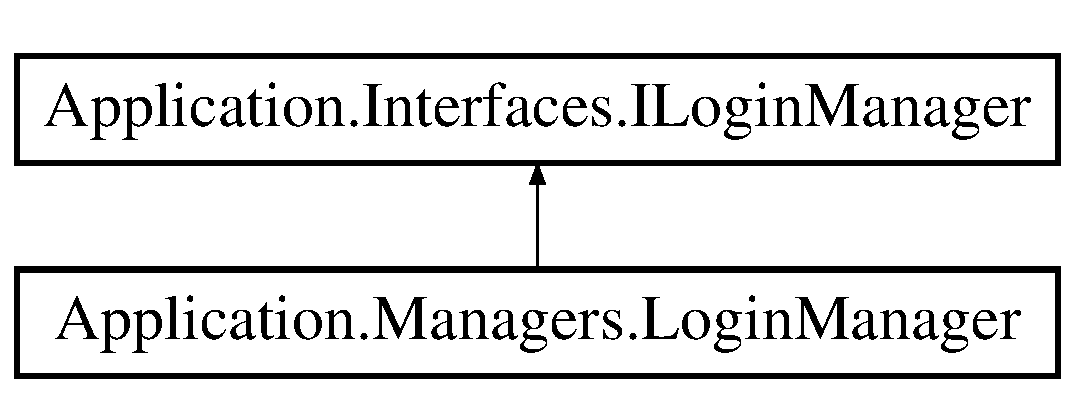
\includegraphics[height=2.000000cm]{class_application_1_1_managers_1_1_login_manager}
\end{center}
\end{figure}
\subsection*{Public Member Functions}
\begin{DoxyCompactItemize}
\item 
void \mbox{\hyperlink{class_application_1_1_managers_1_1_login_manager_a561516fbf8f97f695efdb1cb696899e8}{Login}} (I\+User user)
\begin{DoxyCompactList}\small\item\em Logs in the user \end{DoxyCompactList}\item 
bool \mbox{\hyperlink{class_application_1_1_managers_1_1_login_manager_ab485bd570a5d994461c54eb07e97a43a}{Check\+Login\+Status}} (string username, string password)
\begin{DoxyCompactList}\small\item\em Returns whether the user with username is logged in. If this is the case it updates the users time stamp \end{DoxyCompactList}\item 
bool \mbox{\hyperlink{class_application_1_1_managers_1_1_login_manager_a9502ab9e9e8d04a42a9c3cdf451b405b}{Subscribe\+On\+Log\+Out}} (string username, User\+Logged\+Out\+Handle handle)
\begin{DoxyCompactList}\small\item\em Subscribe to the username with the given handler. If the user is logged out the handler will get called. Make sure to call Check\+Login\+Status prior to this call \end{DoxyCompactList}\item 
bool \mbox{\hyperlink{class_application_1_1_managers_1_1_login_manager_a4490bbdc301ad6eab762fd1a567fd970}{Unsubscribe\+On\+Log\+Out}} (string username, User\+Logged\+Out\+Handle handle)
\begin{DoxyCompactList}\small\item\em Unsubscribes the handler from the username. \end{DoxyCompactList}\item 
\mbox{\hyperlink{class_application_1_1_managers_1_1_login_manager_a22b0fe0bd49da0a911f1cf39a5658d2b}{Login\+Manager}} (\mbox{\hyperlink{interface_application_1_1_interfaces_1_1_i_user_cache}{I\+User\+Cache}} logged\+In\+Pool)
\end{DoxyCompactItemize}
\subsection*{Static Public Member Functions}
\begin{DoxyCompactItemize}
\item 
static \mbox{\hyperlink{interface_application_1_1_interfaces_1_1_i_login_manager}{I\+Login\+Manager}} \mbox{\hyperlink{class_application_1_1_managers_1_1_login_manager_ad9e40fd5ba6a176474a914bb94142ee7}{Get\+Instance}} (\mbox{\hyperlink{interface_application_1_1_interfaces_1_1_i_user_cache}{I\+User\+Cache}} pool=null)
\end{DoxyCompactItemize}


\subsection{Constructor \& Destructor Documentation}
\mbox{\Hypertarget{class_application_1_1_managers_1_1_login_manager_a22b0fe0bd49da0a911f1cf39a5658d2b}\label{class_application_1_1_managers_1_1_login_manager_a22b0fe0bd49da0a911f1cf39a5658d2b}} 
\index{Application\+::\+Managers\+::\+Login\+Manager@{Application\+::\+Managers\+::\+Login\+Manager}!Login\+Manager@{Login\+Manager}}
\index{Login\+Manager@{Login\+Manager}!Application\+::\+Managers\+::\+Login\+Manager@{Application\+::\+Managers\+::\+Login\+Manager}}
\subsubsection{\texorpdfstring{Login\+Manager()}{LoginManager()}}
{\footnotesize\ttfamily Application.\+Managers.\+Login\+Manager.\+Login\+Manager (\begin{DoxyParamCaption}\item[{\mbox{\hyperlink{interface_application_1_1_interfaces_1_1_i_user_cache}{I\+User\+Cache}}}]{logged\+In\+Pool }\end{DoxyParamCaption})}



\subsection{Member Function Documentation}
\mbox{\Hypertarget{class_application_1_1_managers_1_1_login_manager_ab485bd570a5d994461c54eb07e97a43a}\label{class_application_1_1_managers_1_1_login_manager_ab485bd570a5d994461c54eb07e97a43a}} 
\index{Application\+::\+Managers\+::\+Login\+Manager@{Application\+::\+Managers\+::\+Login\+Manager}!Check\+Login\+Status@{Check\+Login\+Status}}
\index{Check\+Login\+Status@{Check\+Login\+Status}!Application\+::\+Managers\+::\+Login\+Manager@{Application\+::\+Managers\+::\+Login\+Manager}}
\subsubsection{\texorpdfstring{Check\+Login\+Status()}{CheckLoginStatus()}}
{\footnotesize\ttfamily bool Application.\+Managers.\+Login\+Manager.\+Check\+Login\+Status (\begin{DoxyParamCaption}\item[{string}]{username,  }\item[{string}]{password }\end{DoxyParamCaption})}



Returns whether the user with username is logged in. If this is the case it updates the users time stamp 


\begin{DoxyParams}{Parameters}
{\em username} & \\
\hline
\end{DoxyParams}
\begin{DoxyReturn}{Returns}

\end{DoxyReturn}


Implements \mbox{\hyperlink{interface_application_1_1_interfaces_1_1_i_login_manager_a31282ac878dc798af1a542f23efc7c8b}{Application.\+Interfaces.\+I\+Login\+Manager}}.

\mbox{\Hypertarget{class_application_1_1_managers_1_1_login_manager_ad9e40fd5ba6a176474a914bb94142ee7}\label{class_application_1_1_managers_1_1_login_manager_ad9e40fd5ba6a176474a914bb94142ee7}} 
\index{Application\+::\+Managers\+::\+Login\+Manager@{Application\+::\+Managers\+::\+Login\+Manager}!Get\+Instance@{Get\+Instance}}
\index{Get\+Instance@{Get\+Instance}!Application\+::\+Managers\+::\+Login\+Manager@{Application\+::\+Managers\+::\+Login\+Manager}}
\subsubsection{\texorpdfstring{Get\+Instance()}{GetInstance()}}
{\footnotesize\ttfamily static \mbox{\hyperlink{interface_application_1_1_interfaces_1_1_i_login_manager}{I\+Login\+Manager}} Application.\+Managers.\+Login\+Manager.\+Get\+Instance (\begin{DoxyParamCaption}\item[{\mbox{\hyperlink{interface_application_1_1_interfaces_1_1_i_user_cache}{I\+User\+Cache}}}]{pool = {\ttfamily null} }\end{DoxyParamCaption})\hspace{0.3cm}{\ttfamily [static]}}

\mbox{\Hypertarget{class_application_1_1_managers_1_1_login_manager_a561516fbf8f97f695efdb1cb696899e8}\label{class_application_1_1_managers_1_1_login_manager_a561516fbf8f97f695efdb1cb696899e8}} 
\index{Application\+::\+Managers\+::\+Login\+Manager@{Application\+::\+Managers\+::\+Login\+Manager}!Login@{Login}}
\index{Login@{Login}!Application\+::\+Managers\+::\+Login\+Manager@{Application\+::\+Managers\+::\+Login\+Manager}}
\subsubsection{\texorpdfstring{Login()}{Login()}}
{\footnotesize\ttfamily void Application.\+Managers.\+Login\+Manager.\+Login (\begin{DoxyParamCaption}\item[{I\+User}]{user }\end{DoxyParamCaption})}



Logs in the user 


\begin{DoxyParams}{Parameters}
{\em user} & \\
\hline
\end{DoxyParams}


Implements \mbox{\hyperlink{interface_application_1_1_interfaces_1_1_i_login_manager_abfad12b55f211087464278f6301ba2e6}{Application.\+Interfaces.\+I\+Login\+Manager}}.

\mbox{\Hypertarget{class_application_1_1_managers_1_1_login_manager_a9502ab9e9e8d04a42a9c3cdf451b405b}\label{class_application_1_1_managers_1_1_login_manager_a9502ab9e9e8d04a42a9c3cdf451b405b}} 
\index{Application\+::\+Managers\+::\+Login\+Manager@{Application\+::\+Managers\+::\+Login\+Manager}!Subscribe\+On\+Log\+Out@{Subscribe\+On\+Log\+Out}}
\index{Subscribe\+On\+Log\+Out@{Subscribe\+On\+Log\+Out}!Application\+::\+Managers\+::\+Login\+Manager@{Application\+::\+Managers\+::\+Login\+Manager}}
\subsubsection{\texorpdfstring{Subscribe\+On\+Log\+Out()}{SubscribeOnLogOut()}}
{\footnotesize\ttfamily bool Application.\+Managers.\+Login\+Manager.\+Subscribe\+On\+Log\+Out (\begin{DoxyParamCaption}\item[{string}]{username,  }\item[{User\+Logged\+Out\+Handle}]{handle }\end{DoxyParamCaption})}



Subscribe to the username with the given handler. If the user is logged out the handler will get called. Make sure to call Check\+Login\+Status prior to this call 


\begin{DoxyParams}{Parameters}
{\em username} & \\
\hline
{\em handle} & \\
\hline
\end{DoxyParams}
\begin{DoxyReturn}{Returns}

\end{DoxyReturn}


Implements \mbox{\hyperlink{interface_application_1_1_interfaces_1_1_i_login_manager_a81fc028c701e8e372d635d6bd9664570}{Application.\+Interfaces.\+I\+Login\+Manager}}.

\mbox{\Hypertarget{class_application_1_1_managers_1_1_login_manager_a4490bbdc301ad6eab762fd1a567fd970}\label{class_application_1_1_managers_1_1_login_manager_a4490bbdc301ad6eab762fd1a567fd970}} 
\index{Application\+::\+Managers\+::\+Login\+Manager@{Application\+::\+Managers\+::\+Login\+Manager}!Unsubscribe\+On\+Log\+Out@{Unsubscribe\+On\+Log\+Out}}
\index{Unsubscribe\+On\+Log\+Out@{Unsubscribe\+On\+Log\+Out}!Application\+::\+Managers\+::\+Login\+Manager@{Application\+::\+Managers\+::\+Login\+Manager}}
\subsubsection{\texorpdfstring{Unsubscribe\+On\+Log\+Out()}{UnsubscribeOnLogOut()}}
{\footnotesize\ttfamily bool Application.\+Managers.\+Login\+Manager.\+Unsubscribe\+On\+Log\+Out (\begin{DoxyParamCaption}\item[{string}]{username,  }\item[{User\+Logged\+Out\+Handle}]{handle }\end{DoxyParamCaption})}



Unsubscribes the handler from the username. 


\begin{DoxyParams}{Parameters}
{\em username} & \\
\hline
{\em handle} & \\
\hline
\end{DoxyParams}
\begin{DoxyReturn}{Returns}

\end{DoxyReturn}


Implements \mbox{\hyperlink{interface_application_1_1_interfaces_1_1_i_login_manager_aeb60a7935fa777e629db6098ce2f458d}{Application.\+Interfaces.\+I\+Login\+Manager}}.



The documentation for this class was generated from the following file\+:\begin{DoxyCompactItemize}
\item 
Managers/\mbox{\hyperlink{_login_manager_8cs}{Login\+Manager.\+cs}}\end{DoxyCompactItemize}

\hypertarget{struct_application_1_1_misc_1_1_smart_lock_1_1_releaser}{}\section{Application.\+Misc.\+Smart\+Lock.\+Releaser Struct Reference}
\label{struct_application_1_1_misc_1_1_smart_lock_1_1_releaser}\index{Application.\+Misc.\+Smart\+Lock.\+Releaser@{Application.\+Misc.\+Smart\+Lock.\+Releaser}}
Inheritance diagram for Application.\+Misc.\+Smart\+Lock.\+Releaser\+:\begin{figure}[H]
\begin{center}
\leavevmode
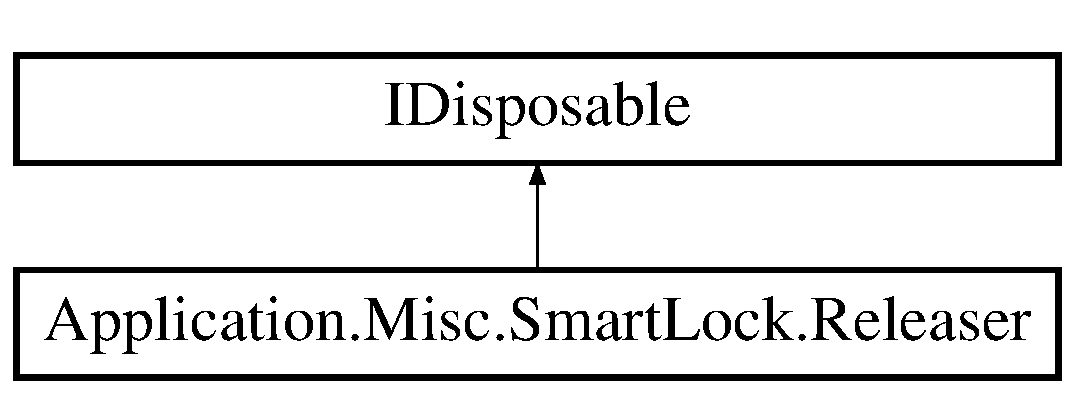
\includegraphics[height=2.000000cm]{struct_application_1_1_misc_1_1_smart_lock_1_1_releaser}
\end{center}
\end{figure}
\subsection*{Public Member Functions}
\begin{DoxyCompactItemize}
\item 
void \mbox{\hyperlink{struct_application_1_1_misc_1_1_smart_lock_1_1_releaser_a373f33cf67fe31aece5a6bf41417bd3c}{Dispose}} ()
\end{DoxyCompactItemize}


\subsection{Member Function Documentation}
\mbox{\Hypertarget{struct_application_1_1_misc_1_1_smart_lock_1_1_releaser_a373f33cf67fe31aece5a6bf41417bd3c}\label{struct_application_1_1_misc_1_1_smart_lock_1_1_releaser_a373f33cf67fe31aece5a6bf41417bd3c}} 
\index{Application\+::\+Misc\+::\+Smart\+Lock\+::\+Releaser@{Application\+::\+Misc\+::\+Smart\+Lock\+::\+Releaser}!Dispose@{Dispose}}
\index{Dispose@{Dispose}!Application\+::\+Misc\+::\+Smart\+Lock\+::\+Releaser@{Application\+::\+Misc\+::\+Smart\+Lock\+::\+Releaser}}
\subsubsection{\texorpdfstring{Dispose()}{Dispose()}}
{\footnotesize\ttfamily void Application.\+Misc.\+Smart\+Lock.\+Releaser.\+Dispose (\begin{DoxyParamCaption}{ }\end{DoxyParamCaption})}



The documentation for this struct was generated from the following file\+:\begin{DoxyCompactItemize}
\item 
Misc/\mbox{\hyperlink{_smart_lock_8cs}{Smart\+Lock.\+cs}}\end{DoxyCompactItemize}

\hypertarget{class_application_1_1_misc_1_1_smart_lock}{}\section{Application.\+Misc.\+Smart\+Lock Class Reference}
\label{class_application_1_1_misc_1_1_smart_lock}\index{Application.\+Misc.\+Smart\+Lock@{Application.\+Misc.\+Smart\+Lock}}


Inspired by\+: \href{https://blogs.msdn.microsoft.com/pfxteam/2012/02/12/building-async-coordination-primitives-part-6-asynclock/}{\tt https\+://blogs.\+msdn.\+microsoft.\+com/pfxteam/2012/02/12/building-\/async-\/coordination-\/primitives-\/part-\/6-\/asynclock/}  


\subsection*{Classes}
\begin{DoxyCompactItemize}
\item 
struct \mbox{\hyperlink{struct_application_1_1_misc_1_1_smart_lock_1_1_releaser}{Releaser}}
\end{DoxyCompactItemize}
\subsection*{Public Member Functions}
\begin{DoxyCompactItemize}
\item 
\mbox{\hyperlink{class_application_1_1_misc_1_1_smart_lock_a0457fe6081ff3c8eec2afa42ed24bc8f}{Smart\+Lock}} ()
\item 
Task$<$ \mbox{\hyperlink{struct_application_1_1_misc_1_1_smart_lock_1_1_releaser}{Releaser}} $>$ \mbox{\hyperlink{class_application_1_1_misc_1_1_smart_lock_af850c4ff0257ebcd9318688e13204e91}{Lock\+Async}} ()
\item 
\mbox{\hyperlink{struct_application_1_1_misc_1_1_smart_lock_1_1_releaser}{Releaser}} \mbox{\hyperlink{class_application_1_1_misc_1_1_smart_lock_a10db87dc210c66e3760ebcdb897b4522}{Lock}} ()
\end{DoxyCompactItemize}


\subsection{Detailed Description}
Inspired by\+: \href{https://blogs.msdn.microsoft.com/pfxteam/2012/02/12/building-async-coordination-primitives-part-6-asynclock/}{\tt https\+://blogs.\+msdn.\+microsoft.\+com/pfxteam/2012/02/12/building-\/async-\/coordination-\/primitives-\/part-\/6-\/asynclock/} 



\subsection{Constructor \& Destructor Documentation}
\mbox{\Hypertarget{class_application_1_1_misc_1_1_smart_lock_a0457fe6081ff3c8eec2afa42ed24bc8f}\label{class_application_1_1_misc_1_1_smart_lock_a0457fe6081ff3c8eec2afa42ed24bc8f}} 
\index{Application\+::\+Misc\+::\+Smart\+Lock@{Application\+::\+Misc\+::\+Smart\+Lock}!Smart\+Lock@{Smart\+Lock}}
\index{Smart\+Lock@{Smart\+Lock}!Application\+::\+Misc\+::\+Smart\+Lock@{Application\+::\+Misc\+::\+Smart\+Lock}}
\subsubsection{\texorpdfstring{Smart\+Lock()}{SmartLock()}}
{\footnotesize\ttfamily Application.\+Misc.\+Smart\+Lock.\+Smart\+Lock (\begin{DoxyParamCaption}{ }\end{DoxyParamCaption})}



\subsection{Member Function Documentation}
\mbox{\Hypertarget{class_application_1_1_misc_1_1_smart_lock_a10db87dc210c66e3760ebcdb897b4522}\label{class_application_1_1_misc_1_1_smart_lock_a10db87dc210c66e3760ebcdb897b4522}} 
\index{Application\+::\+Misc\+::\+Smart\+Lock@{Application\+::\+Misc\+::\+Smart\+Lock}!Lock@{Lock}}
\index{Lock@{Lock}!Application\+::\+Misc\+::\+Smart\+Lock@{Application\+::\+Misc\+::\+Smart\+Lock}}
\subsubsection{\texorpdfstring{Lock()}{Lock()}}
{\footnotesize\ttfamily \mbox{\hyperlink{struct_application_1_1_misc_1_1_smart_lock_1_1_releaser}{Releaser}} Application.\+Misc.\+Smart\+Lock.\+Lock (\begin{DoxyParamCaption}{ }\end{DoxyParamCaption})}

\mbox{\Hypertarget{class_application_1_1_misc_1_1_smart_lock_af850c4ff0257ebcd9318688e13204e91}\label{class_application_1_1_misc_1_1_smart_lock_af850c4ff0257ebcd9318688e13204e91}} 
\index{Application\+::\+Misc\+::\+Smart\+Lock@{Application\+::\+Misc\+::\+Smart\+Lock}!Lock\+Async@{Lock\+Async}}
\index{Lock\+Async@{Lock\+Async}!Application\+::\+Misc\+::\+Smart\+Lock@{Application\+::\+Misc\+::\+Smart\+Lock}}
\subsubsection{\texorpdfstring{Lock\+Async()}{LockAsync()}}
{\footnotesize\ttfamily Task$<$\mbox{\hyperlink{struct_application_1_1_misc_1_1_smart_lock_1_1_releaser}{Releaser}}$>$ Application.\+Misc.\+Smart\+Lock.\+Lock\+Async (\begin{DoxyParamCaption}{ }\end{DoxyParamCaption})}



The documentation for this class was generated from the following file\+:\begin{DoxyCompactItemize}
\item 
Misc/\mbox{\hyperlink{_smart_lock_8cs}{Smart\+Lock.\+cs}}\end{DoxyCompactItemize}

\hypertarget{class_application_1_1_interfaces_1_1_timed_out_user_event_args}{}\section{Application.\+Interfaces.\+Timed\+Out\+User\+Event\+Args Class Reference}
\label{class_application_1_1_interfaces_1_1_timed_out_user_event_args}\index{Application.\+Interfaces.\+Timed\+Out\+User\+Event\+Args@{Application.\+Interfaces.\+Timed\+Out\+User\+Event\+Args}}
Inheritance diagram for Application.\+Interfaces.\+Timed\+Out\+User\+Event\+Args\+:\begin{figure}[H]
\begin{center}
\leavevmode
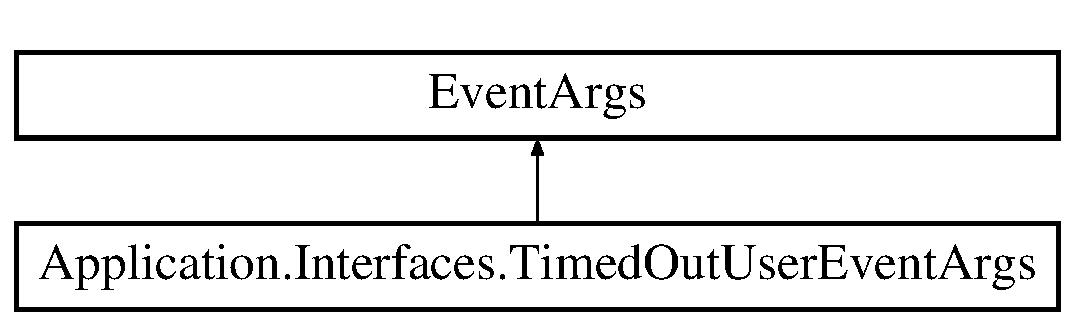
\includegraphics[height=2.000000cm]{class_application_1_1_interfaces_1_1_timed_out_user_event_args}
\end{center}
\end{figure}
\subsection*{Public Member Functions}
\begin{DoxyCompactItemize}
\item 
\mbox{\hyperlink{class_application_1_1_interfaces_1_1_timed_out_user_event_args_ad70d0e4500f69bf4459ef76d86e5412d}{Timed\+Out\+User\+Event\+Args}} (string username)
\end{DoxyCompactItemize}
\subsection*{Properties}
\begin{DoxyCompactItemize}
\item 
string \mbox{\hyperlink{class_application_1_1_interfaces_1_1_timed_out_user_event_args_ad359e7a3cc388ea94e1332e9109cebf8}{Timed\+Out\+Username}}\hspace{0.3cm}{\ttfamily  \mbox{[}get\mbox{]}}
\end{DoxyCompactItemize}


\subsection{Constructor \& Destructor Documentation}
\mbox{\Hypertarget{class_application_1_1_interfaces_1_1_timed_out_user_event_args_ad70d0e4500f69bf4459ef76d86e5412d}\label{class_application_1_1_interfaces_1_1_timed_out_user_event_args_ad70d0e4500f69bf4459ef76d86e5412d}} 
\index{Application\+::\+Interfaces\+::\+Timed\+Out\+User\+Event\+Args@{Application\+::\+Interfaces\+::\+Timed\+Out\+User\+Event\+Args}!Timed\+Out\+User\+Event\+Args@{Timed\+Out\+User\+Event\+Args}}
\index{Timed\+Out\+User\+Event\+Args@{Timed\+Out\+User\+Event\+Args}!Application\+::\+Interfaces\+::\+Timed\+Out\+User\+Event\+Args@{Application\+::\+Interfaces\+::\+Timed\+Out\+User\+Event\+Args}}
\subsubsection{\texorpdfstring{Timed\+Out\+User\+Event\+Args()}{TimedOutUserEventArgs()}}
{\footnotesize\ttfamily Application.\+Interfaces.\+Timed\+Out\+User\+Event\+Args.\+Timed\+Out\+User\+Event\+Args (\begin{DoxyParamCaption}\item[{string}]{username }\end{DoxyParamCaption})}



\subsection{Property Documentation}
\mbox{\Hypertarget{class_application_1_1_interfaces_1_1_timed_out_user_event_args_ad359e7a3cc388ea94e1332e9109cebf8}\label{class_application_1_1_interfaces_1_1_timed_out_user_event_args_ad359e7a3cc388ea94e1332e9109cebf8}} 
\index{Application\+::\+Interfaces\+::\+Timed\+Out\+User\+Event\+Args@{Application\+::\+Interfaces\+::\+Timed\+Out\+User\+Event\+Args}!Timed\+Out\+Username@{Timed\+Out\+Username}}
\index{Timed\+Out\+Username@{Timed\+Out\+Username}!Application\+::\+Interfaces\+::\+Timed\+Out\+User\+Event\+Args@{Application\+::\+Interfaces\+::\+Timed\+Out\+User\+Event\+Args}}
\subsubsection{\texorpdfstring{Timed\+Out\+Username}{TimedOutUsername}}
{\footnotesize\ttfamily string Application.\+Interfaces.\+Timed\+Out\+User\+Event\+Args.\+Timed\+Out\+Username\hspace{0.3cm}{\ttfamily [get]}}



The documentation for this class was generated from the following file\+:\begin{DoxyCompactItemize}
\item 
Interfaces/\mbox{\hyperlink{_i_user_cache_8cs}{I\+User\+Cache.\+cs}}\end{DoxyCompactItemize}

\hypertarget{class_application_1_1_misc_1_1_user_cache}{}\section{Application.\+Misc.\+User\+Cache Class Reference}
\label{class_application_1_1_misc_1_1_user_cache}\index{Application.\+Misc.\+User\+Cache@{Application.\+Misc.\+User\+Cache}}
Inheritance diagram for Application.\+Misc.\+User\+Cache\+:\begin{figure}[H]
\begin{center}
\leavevmode
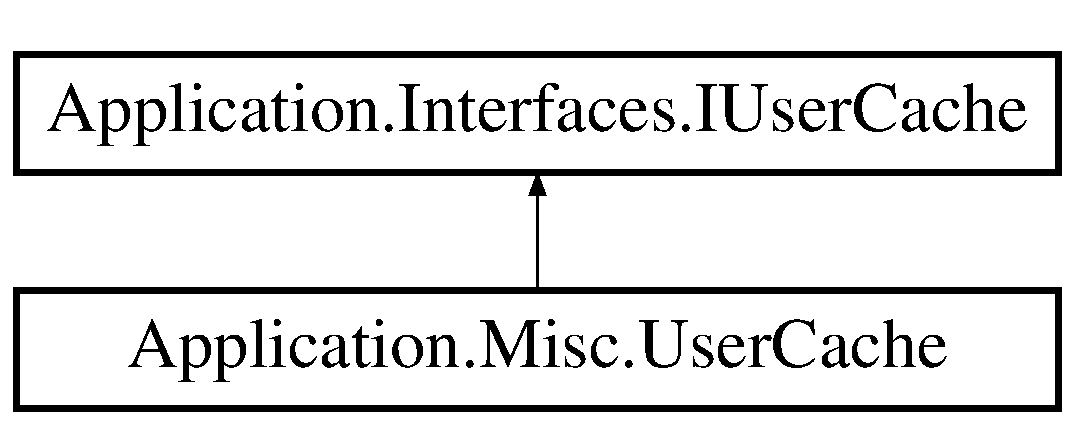
\includegraphics[height=2.000000cm]{class_application_1_1_misc_1_1_user_cache}
\end{center}
\end{figure}
\subsection*{Public Member Functions}
\begin{DoxyCompactItemize}
\item 
\mbox{\hyperlink{class_application_1_1_misc_1_1_user_cache_ab52d91840d3b6c3d4162992b35bbf3a5}{User\+Cache}} (\mbox{\hyperlink{interface_application_1_1_interfaces_1_1_i_timer}{I\+Timer}} timer)
\item 
void \mbox{\hyperlink{class_application_1_1_misc_1_1_user_cache_ab56ecb52b9a7bc855729b439a5c5bb36}{Add\+Or\+Update}} (string username, string password)
\begin{DoxyCompactList}\small\item\em Adds a user to the cache with the default timeout of 20 minutes. \end{DoxyCompactList}\item 
void \mbox{\hyperlink{class_application_1_1_misc_1_1_user_cache_a7c8d6acdc76809a72a36db8ba8fdd8f8}{Add\+Or\+Update}} (string username, string password, Date\+Time timeout)
\begin{DoxyCompactList}\small\item\em Adds a user to the cache with the timeout given in the paramater timeout. \end{DoxyCompactList}\item 
bool \mbox{\hyperlink{class_application_1_1_misc_1_1_user_cache_a77b10de2cba0f07aa9af6fd5ad53e2c6}{Confirm}} (string username)
\begin{DoxyCompactList}\small\item\em Confirms that the user is currently in the cache. Does N\+OT refresh his timeout. \end{DoxyCompactList}\item 
bool \mbox{\hyperlink{class_application_1_1_misc_1_1_user_cache_ad11a0422af31b1492098415d8e4aaad8}{Confirm\+And\+Refresh}} (string username, string password)
\begin{DoxyCompactList}\small\item\em Confirms that the user is currenty in the cache and if so refreshes the user\textquotesingle{}s timeout. The password must match. Returns true if user is found and refreshed, else false. \end{DoxyCompactList}\item 
bool \mbox{\hyperlink{class_application_1_1_misc_1_1_user_cache_af685f56bf378e2bde07f7f6f933a8e0e}{Remove}} (string username, string password)
\begin{DoxyCompactList}\small\item\em Removes the user from the cache. Returns true if succesful. Else false. \end{DoxyCompactList}\end{DoxyCompactItemize}
\subsection*{Properties}
\begin{DoxyCompactItemize}
\item 
I\+Read\+Only\+Dictionary$<$ string, Date\+Time $>$ \mbox{\hyperlink{class_application_1_1_misc_1_1_user_cache_ad5b655841c5a15022a372cfe9fb6960d}{Expiration\+Stamps}}\hspace{0.3cm}{\ttfamily  \mbox{[}get\mbox{]}}
\begin{DoxyCompactList}\small\item\em This was added for unit-\/testing purposes. This is not thread-\/safe and should not be used for anything other than testing Will return a dictionary with usernames as keys and the value coresponding to the timeout of the user \end{DoxyCompactList}\end{DoxyCompactItemize}
\subsection*{Events}
\begin{DoxyCompactItemize}
\item 
Event\+Handler$<$ \mbox{\hyperlink{class_application_1_1_interfaces_1_1_timed_out_user_event_args}{Timed\+Out\+User\+Event\+Args}} $>$ \mbox{\hyperlink{class_application_1_1_misc_1_1_user_cache_aac04127fb652a14238e2742d0bba6558}{Users\+Timed\+Out\+Event}}
\end{DoxyCompactItemize}


\subsection{Constructor \& Destructor Documentation}
\mbox{\Hypertarget{class_application_1_1_misc_1_1_user_cache_ab52d91840d3b6c3d4162992b35bbf3a5}\label{class_application_1_1_misc_1_1_user_cache_ab52d91840d3b6c3d4162992b35bbf3a5}} 
\index{Application\+::\+Misc\+::\+User\+Cache@{Application\+::\+Misc\+::\+User\+Cache}!User\+Cache@{User\+Cache}}
\index{User\+Cache@{User\+Cache}!Application\+::\+Misc\+::\+User\+Cache@{Application\+::\+Misc\+::\+User\+Cache}}
\subsubsection{\texorpdfstring{User\+Cache()}{UserCache()}}
{\footnotesize\ttfamily Application.\+Misc.\+User\+Cache.\+User\+Cache (\begin{DoxyParamCaption}\item[{\mbox{\hyperlink{interface_application_1_1_interfaces_1_1_i_timer}{I\+Timer}}}]{timer }\end{DoxyParamCaption})}



\subsection{Member Function Documentation}
\mbox{\Hypertarget{class_application_1_1_misc_1_1_user_cache_ab56ecb52b9a7bc855729b439a5c5bb36}\label{class_application_1_1_misc_1_1_user_cache_ab56ecb52b9a7bc855729b439a5c5bb36}} 
\index{Application\+::\+Misc\+::\+User\+Cache@{Application\+::\+Misc\+::\+User\+Cache}!Add\+Or\+Update@{Add\+Or\+Update}}
\index{Add\+Or\+Update@{Add\+Or\+Update}!Application\+::\+Misc\+::\+User\+Cache@{Application\+::\+Misc\+::\+User\+Cache}}
\subsubsection{\texorpdfstring{Add\+Or\+Update()}{AddOrUpdate()}\hspace{0.1cm}{\footnotesize\ttfamily [1/2]}}
{\footnotesize\ttfamily void Application.\+Misc.\+User\+Cache.\+Add\+Or\+Update (\begin{DoxyParamCaption}\item[{string}]{username,  }\item[{string}]{password }\end{DoxyParamCaption})}



Adds a user to the cache with the default timeout of 20 minutes. 


\begin{DoxyParams}{Parameters}
{\em username} & Username of user\\
\hline
{\em password} & password of user\\
\hline
\end{DoxyParams}
\begin{DoxyReturn}{Returns}

\end{DoxyReturn}


Implements \mbox{\hyperlink{interface_application_1_1_interfaces_1_1_i_user_cache_a607deb5ebf1cfb0f237daf9981206d73}{Application.\+Interfaces.\+I\+User\+Cache}}.

\mbox{\Hypertarget{class_application_1_1_misc_1_1_user_cache_a7c8d6acdc76809a72a36db8ba8fdd8f8}\label{class_application_1_1_misc_1_1_user_cache_a7c8d6acdc76809a72a36db8ba8fdd8f8}} 
\index{Application\+::\+Misc\+::\+User\+Cache@{Application\+::\+Misc\+::\+User\+Cache}!Add\+Or\+Update@{Add\+Or\+Update}}
\index{Add\+Or\+Update@{Add\+Or\+Update}!Application\+::\+Misc\+::\+User\+Cache@{Application\+::\+Misc\+::\+User\+Cache}}
\subsubsection{\texorpdfstring{Add\+Or\+Update()}{AddOrUpdate()}\hspace{0.1cm}{\footnotesize\ttfamily [2/2]}}
{\footnotesize\ttfamily void Application.\+Misc.\+User\+Cache.\+Add\+Or\+Update (\begin{DoxyParamCaption}\item[{string}]{username,  }\item[{string}]{password,  }\item[{Date\+Time}]{timeout }\end{DoxyParamCaption})}



Adds a user to the cache with the timeout given in the paramater timeout. 


\begin{DoxyParams}{Parameters}
{\em username} & Username of user\\
\hline
{\em password} & password of user\\
\hline
{\em timeout} & \\
\hline
\end{DoxyParams}
\begin{DoxyReturn}{Returns}

\end{DoxyReturn}


Implements \mbox{\hyperlink{interface_application_1_1_interfaces_1_1_i_user_cache_aec631e3f0e466a067018b3196457056a}{Application.\+Interfaces.\+I\+User\+Cache}}.

\mbox{\Hypertarget{class_application_1_1_misc_1_1_user_cache_a77b10de2cba0f07aa9af6fd5ad53e2c6}\label{class_application_1_1_misc_1_1_user_cache_a77b10de2cba0f07aa9af6fd5ad53e2c6}} 
\index{Application\+::\+Misc\+::\+User\+Cache@{Application\+::\+Misc\+::\+User\+Cache}!Confirm@{Confirm}}
\index{Confirm@{Confirm}!Application\+::\+Misc\+::\+User\+Cache@{Application\+::\+Misc\+::\+User\+Cache}}
\subsubsection{\texorpdfstring{Confirm()}{Confirm()}}
{\footnotesize\ttfamily bool Application.\+Misc.\+User\+Cache.\+Confirm (\begin{DoxyParamCaption}\item[{string}]{username }\end{DoxyParamCaption})}



Confirms that the user is currently in the cache. Does N\+OT refresh his timeout. 


\begin{DoxyParams}{Parameters}
{\em username} & \\
\hline
\end{DoxyParams}
\begin{DoxyReturn}{Returns}

\end{DoxyReturn}


Implements \mbox{\hyperlink{interface_application_1_1_interfaces_1_1_i_user_cache_a4978aad56d7292eafa02e8e7ad66f2c2}{Application.\+Interfaces.\+I\+User\+Cache}}.

\mbox{\Hypertarget{class_application_1_1_misc_1_1_user_cache_ad11a0422af31b1492098415d8e4aaad8}\label{class_application_1_1_misc_1_1_user_cache_ad11a0422af31b1492098415d8e4aaad8}} 
\index{Application\+::\+Misc\+::\+User\+Cache@{Application\+::\+Misc\+::\+User\+Cache}!Confirm\+And\+Refresh@{Confirm\+And\+Refresh}}
\index{Confirm\+And\+Refresh@{Confirm\+And\+Refresh}!Application\+::\+Misc\+::\+User\+Cache@{Application\+::\+Misc\+::\+User\+Cache}}
\subsubsection{\texorpdfstring{Confirm\+And\+Refresh()}{ConfirmAndRefresh()}}
{\footnotesize\ttfamily bool Application.\+Misc.\+User\+Cache.\+Confirm\+And\+Refresh (\begin{DoxyParamCaption}\item[{string}]{username,  }\item[{string}]{password }\end{DoxyParamCaption})}



Confirms that the user is currenty in the cache and if so refreshes the user\textquotesingle{}s timeout. The password must match. Returns true if user is found and refreshed, else false. 


\begin{DoxyParams}{Parameters}
{\em username} & \\
\hline
{\em password} & \\
\hline
\end{DoxyParams}
\begin{DoxyReturn}{Returns}

\end{DoxyReturn}


Implements \mbox{\hyperlink{interface_application_1_1_interfaces_1_1_i_user_cache_a3516a7abf1f40f9ddd10243cad03bb65}{Application.\+Interfaces.\+I\+User\+Cache}}.

\mbox{\Hypertarget{class_application_1_1_misc_1_1_user_cache_af685f56bf378e2bde07f7f6f933a8e0e}\label{class_application_1_1_misc_1_1_user_cache_af685f56bf378e2bde07f7f6f933a8e0e}} 
\index{Application\+::\+Misc\+::\+User\+Cache@{Application\+::\+Misc\+::\+User\+Cache}!Remove@{Remove}}
\index{Remove@{Remove}!Application\+::\+Misc\+::\+User\+Cache@{Application\+::\+Misc\+::\+User\+Cache}}
\subsubsection{\texorpdfstring{Remove()}{Remove()}}
{\footnotesize\ttfamily bool Application.\+Misc.\+User\+Cache.\+Remove (\begin{DoxyParamCaption}\item[{string}]{username,  }\item[{string}]{password }\end{DoxyParamCaption})}



Removes the user from the cache. Returns true if succesful. Else false. 


\begin{DoxyParams}{Parameters}
{\em username} & \\
\hline
{\em password} & \\
\hline
\end{DoxyParams}
\begin{DoxyReturn}{Returns}

\end{DoxyReturn}


Implements \mbox{\hyperlink{interface_application_1_1_interfaces_1_1_i_user_cache_ac8ccbf20ac25069528e1e5117d5481ee}{Application.\+Interfaces.\+I\+User\+Cache}}.



\subsection{Property Documentation}
\mbox{\Hypertarget{class_application_1_1_misc_1_1_user_cache_ad5b655841c5a15022a372cfe9fb6960d}\label{class_application_1_1_misc_1_1_user_cache_ad5b655841c5a15022a372cfe9fb6960d}} 
\index{Application\+::\+Misc\+::\+User\+Cache@{Application\+::\+Misc\+::\+User\+Cache}!Expiration\+Stamps@{Expiration\+Stamps}}
\index{Expiration\+Stamps@{Expiration\+Stamps}!Application\+::\+Misc\+::\+User\+Cache@{Application\+::\+Misc\+::\+User\+Cache}}
\subsubsection{\texorpdfstring{Expiration\+Stamps}{ExpirationStamps}}
{\footnotesize\ttfamily I\+Read\+Only\+Dictionary$<$string, Date\+Time$>$ Application.\+Misc.\+User\+Cache.\+Expiration\+Stamps\hspace{0.3cm}{\ttfamily [get]}}



This was added for unit-\/testing purposes. This is not thread-\/safe and should not be used for anything other than testing Will return a dictionary with usernames as keys and the value coresponding to the timeout of the user 



\subsection{Event Documentation}
\mbox{\Hypertarget{class_application_1_1_misc_1_1_user_cache_aac04127fb652a14238e2742d0bba6558}\label{class_application_1_1_misc_1_1_user_cache_aac04127fb652a14238e2742d0bba6558}} 
\index{Application\+::\+Misc\+::\+User\+Cache@{Application\+::\+Misc\+::\+User\+Cache}!Users\+Timed\+Out\+Event@{Users\+Timed\+Out\+Event}}
\index{Users\+Timed\+Out\+Event@{Users\+Timed\+Out\+Event}!Application\+::\+Misc\+::\+User\+Cache@{Application\+::\+Misc\+::\+User\+Cache}}
\subsubsection{\texorpdfstring{Users\+Timed\+Out\+Event}{UsersTimedOutEvent}}
{\footnotesize\ttfamily Event\+Handler$<$\mbox{\hyperlink{class_application_1_1_interfaces_1_1_timed_out_user_event_args}{Timed\+Out\+User\+Event\+Args}}$>$ Application.\+Misc.\+User\+Cache.\+Users\+Timed\+Out\+Event}



The documentation for this class was generated from the following file\+:\begin{DoxyCompactItemize}
\item 
Misc/\mbox{\hyperlink{_user_cache_8cs}{User\+Cache.\+cs}}\end{DoxyCompactItemize}

\hypertarget{class_application_1_1_controllers_1_1_user_controller}{}\section{Application.\+Controllers.\+User\+Controller Class Reference}
\label{class_application_1_1_controllers_1_1_user_controller}\index{Application.\+Controllers.\+User\+Controller@{Application.\+Controllers.\+User\+Controller}}


\mbox{\hyperlink{namespace_application}{Application}} User Controller The main purpose of this class is to decouple the framework from our application logic  


Inheritance diagram for Application.\+Controllers.\+User\+Controller\+:\begin{figure}[H]
\begin{center}
\leavevmode
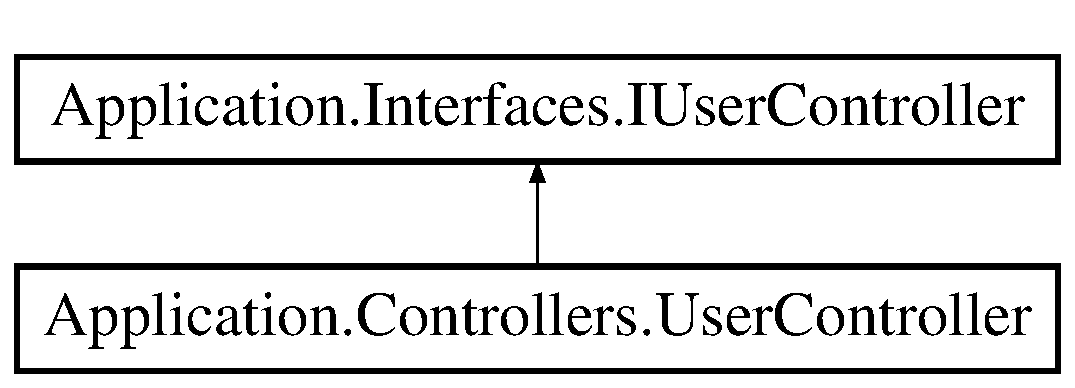
\includegraphics[height=2.000000cm]{class_application_1_1_controllers_1_1_user_controller}
\end{center}
\end{figure}
\subsection*{Public Member Functions}
\begin{DoxyCompactItemize}
\item 
\mbox{\hyperlink{class_application_1_1_controllers_1_1_user_controller_aedfae5fded8199d832e92294b088e418}{User\+Controller}} (I\+User\+Repository user\+Repository, \mbox{\hyperlink{interface_application_1_1_interfaces_1_1_i_login_manager}{I\+Login\+Manager}} login\+Manager)
\item 
I\+User \mbox{\hyperlink{class_application_1_1_controllers_1_1_user_controller_adb2565915559692fae6a146d23d5fe01}{Get\+User}} (string username, string password)
\begin{DoxyCompactList}\small\item\em Returns the user with the given username and password. Null if not found \end{DoxyCompactList}\item 
I\+User \mbox{\hyperlink{class_application_1_1_controllers_1_1_user_controller_abf08955a5adc363fa137399a961a14fc}{Create\+User}} (I\+User user)
\begin{DoxyCompactList}\small\item\em Creates a new user to be stored in the database. Returns valid user upon succes. Otherwise null \end{DoxyCompactList}\item 
I\+User \mbox{\hyperlink{class_application_1_1_controllers_1_1_user_controller_af509b1d73f3a654edfb48dcc1f623ca8}{Update\+User}} (string username, I\+User user)
\begin{DoxyCompactList}\small\item\em Updates the user as given by username and password. Will return null if unsuccesfull \end{DoxyCompactList}\end{DoxyCompactItemize}


\subsection{Detailed Description}
\mbox{\hyperlink{namespace_application}{Application}} User Controller The main purpose of this class is to decouple the framework from our application logic 



\subsection{Constructor \& Destructor Documentation}
\mbox{\Hypertarget{class_application_1_1_controllers_1_1_user_controller_aedfae5fded8199d832e92294b088e418}\label{class_application_1_1_controllers_1_1_user_controller_aedfae5fded8199d832e92294b088e418}} 
\index{Application\+::\+Controllers\+::\+User\+Controller@{Application\+::\+Controllers\+::\+User\+Controller}!User\+Controller@{User\+Controller}}
\index{User\+Controller@{User\+Controller}!Application\+::\+Controllers\+::\+User\+Controller@{Application\+::\+Controllers\+::\+User\+Controller}}
\subsubsection{\texorpdfstring{User\+Controller()}{UserController()}}
{\footnotesize\ttfamily Application.\+Controllers.\+User\+Controller.\+User\+Controller (\begin{DoxyParamCaption}\item[{I\+User\+Repository}]{user\+Repository,  }\item[{\mbox{\hyperlink{interface_application_1_1_interfaces_1_1_i_login_manager}{I\+Login\+Manager}}}]{login\+Manager }\end{DoxyParamCaption})}



\subsection{Member Function Documentation}
\mbox{\Hypertarget{class_application_1_1_controllers_1_1_user_controller_abf08955a5adc363fa137399a961a14fc}\label{class_application_1_1_controllers_1_1_user_controller_abf08955a5adc363fa137399a961a14fc}} 
\index{Application\+::\+Controllers\+::\+User\+Controller@{Application\+::\+Controllers\+::\+User\+Controller}!Create\+User@{Create\+User}}
\index{Create\+User@{Create\+User}!Application\+::\+Controllers\+::\+User\+Controller@{Application\+::\+Controllers\+::\+User\+Controller}}
\subsubsection{\texorpdfstring{Create\+User()}{CreateUser()}}
{\footnotesize\ttfamily I\+User Application.\+Controllers.\+User\+Controller.\+Create\+User (\begin{DoxyParamCaption}\item[{I\+User}]{user }\end{DoxyParamCaption})}



Creates a new user to be stored in the database. Returns valid user upon succes. Otherwise null 


\begin{DoxyParams}{Parameters}
{\em user} & User to be stored\\
\hline
\end{DoxyParams}
\begin{DoxyReturn}{Returns}

\end{DoxyReturn}


Implements \mbox{\hyperlink{interface_application_1_1_interfaces_1_1_i_user_controller_aca064ba3a4c3c2d0dd1339b8a4995e86}{Application.\+Interfaces.\+I\+User\+Controller}}.

\mbox{\Hypertarget{class_application_1_1_controllers_1_1_user_controller_adb2565915559692fae6a146d23d5fe01}\label{class_application_1_1_controllers_1_1_user_controller_adb2565915559692fae6a146d23d5fe01}} 
\index{Application\+::\+Controllers\+::\+User\+Controller@{Application\+::\+Controllers\+::\+User\+Controller}!Get\+User@{Get\+User}}
\index{Get\+User@{Get\+User}!Application\+::\+Controllers\+::\+User\+Controller@{Application\+::\+Controllers\+::\+User\+Controller}}
\subsubsection{\texorpdfstring{Get\+User()}{GetUser()}}
{\footnotesize\ttfamily I\+User Application.\+Controllers.\+User\+Controller.\+Get\+User (\begin{DoxyParamCaption}\item[{string}]{username,  }\item[{string}]{password }\end{DoxyParamCaption})}



Returns the user with the given username and password. Null if not found 


\begin{DoxyParams}{Parameters}
{\em username} & Username of requested user\\
\hline
{\em password} & Password of requested user\\
\hline
\end{DoxyParams}
\begin{DoxyReturn}{Returns}
User
\end{DoxyReturn}


Implements \mbox{\hyperlink{interface_application_1_1_interfaces_1_1_i_user_controller_afdea9f68822192392d4b973e300f56af}{Application.\+Interfaces.\+I\+User\+Controller}}.

\mbox{\Hypertarget{class_application_1_1_controllers_1_1_user_controller_af509b1d73f3a654edfb48dcc1f623ca8}\label{class_application_1_1_controllers_1_1_user_controller_af509b1d73f3a654edfb48dcc1f623ca8}} 
\index{Application\+::\+Controllers\+::\+User\+Controller@{Application\+::\+Controllers\+::\+User\+Controller}!Update\+User@{Update\+User}}
\index{Update\+User@{Update\+User}!Application\+::\+Controllers\+::\+User\+Controller@{Application\+::\+Controllers\+::\+User\+Controller}}
\subsubsection{\texorpdfstring{Update\+User()}{UpdateUser()}}
{\footnotesize\ttfamily I\+User Application.\+Controllers.\+User\+Controller.\+Update\+User (\begin{DoxyParamCaption}\item[{string}]{username,  }\item[{I\+User}]{user }\end{DoxyParamCaption})}



Updates the user as given by username and password. Will return null if unsuccesfull 


\begin{DoxyParams}{Parameters}
{\em username} & Username of user to be updated\\
\hline
{\em user} & User object containing updated information\\
\hline
\end{DoxyParams}
\begin{DoxyReturn}{Returns}

\end{DoxyReturn}


Implements \mbox{\hyperlink{interface_application_1_1_interfaces_1_1_i_user_controller_a433f4021d60dafe735aff4d4b5536370}{Application.\+Interfaces.\+I\+User\+Controller}}.



The documentation for this class was generated from the following file\+:\begin{DoxyCompactItemize}
\item 
Controllers/\mbox{\hyperlink{_user_controller_8cs}{User\+Controller.\+cs}}\end{DoxyCompactItemize}

\chapter{File Documentation}
\hypertarget{_game_controller_8cs}{}\section{Controllers/\+Game\+Controller.cs File Reference}
\label{_game_controller_8cs}\index{Controllers/\+Game\+Controller.\+cs@{Controllers/\+Game\+Controller.\+cs}}
\subsection*{Classes}
\begin{DoxyCompactItemize}
\item 
class \mbox{\hyperlink{class_application_1_1_controllers_1_1_game_controller}{Application.\+Controllers.\+Game\+Controller}}
\end{DoxyCompactItemize}
\subsection*{Namespaces}
\begin{DoxyCompactItemize}
\item 
namespace \mbox{\hyperlink{namespace_application_1_1_controllers}{Application.\+Controllers}}
\end{DoxyCompactItemize}

\hypertarget{_lobby_controller_8cs}{}\section{R\+E\+S\+T\+Controllers/\+Lobby\+Controller.cs File Reference}
\label{_lobby_controller_8cs}\index{R\+E\+S\+T\+Controllers/\+Lobby\+Controller.\+cs@{R\+E\+S\+T\+Controllers/\+Lobby\+Controller.\+cs}}
\subsection*{Classes}
\begin{DoxyCompactItemize}
\item 
class \mbox{\hyperlink{class_communication_1_1_r_e_s_t_controllers_1_1_lobby_controller}{Communication.\+R\+E\+S\+T\+Controllers.\+Lobby\+Controller}}
\end{DoxyCompactItemize}
\subsection*{Namespaces}
\begin{DoxyCompactItemize}
\item 
namespace \mbox{\hyperlink{namespace_communication_1_1_r_e_s_t_controllers}{Communication.\+R\+E\+S\+T\+Controllers}}
\end{DoxyCompactItemize}

\hypertarget{_user_controller_8cs}{}\section{Controllers/\+User\+Controller.cs File Reference}
\label{_user_controller_8cs}\index{Controllers/\+User\+Controller.\+cs@{Controllers/\+User\+Controller.\+cs}}
\subsection*{Classes}
\begin{DoxyCompactItemize}
\item 
class \mbox{\hyperlink{class_application_1_1_controllers_1_1_user_controller}{Application.\+Controllers.\+User\+Controller}}
\begin{DoxyCompactList}\small\item\em \mbox{\hyperlink{namespace_application}{Application}} User Controller The main purpose of this class is to decouple the framework from our application logic \end{DoxyCompactList}\end{DoxyCompactItemize}
\subsection*{Namespaces}
\begin{DoxyCompactItemize}
\item 
namespace \mbox{\hyperlink{namespace_application_1_1_controllers}{Application.\+Controllers}}
\end{DoxyCompactItemize}

\hypertarget{_i_game_controller_8cs}{}\section{Interfaces/\+I\+Game\+Controller.cs File Reference}
\label{_i_game_controller_8cs}\index{Interfaces/\+I\+Game\+Controller.\+cs@{Interfaces/\+I\+Game\+Controller.\+cs}}
\subsection*{Classes}
\begin{DoxyCompactItemize}
\item 
interface \mbox{\hyperlink{interface_application_1_1_interfaces_1_1_i_game_controller}{Application.\+Interfaces.\+I\+Game\+Controller}}
\end{DoxyCompactItemize}
\subsection*{Namespaces}
\begin{DoxyCompactItemize}
\item 
namespace \mbox{\hyperlink{namespace_application_1_1_interfaces}{Application.\+Interfaces}}
\end{DoxyCompactItemize}

\hypertarget{_i_lobby_controller_8cs}{}\section{Interfaces/\+I\+Lobby\+Controller.cs File Reference}
\label{_i_lobby_controller_8cs}\index{Interfaces/\+I\+Lobby\+Controller.\+cs@{Interfaces/\+I\+Lobby\+Controller.\+cs}}
\subsection*{Classes}
\begin{DoxyCompactItemize}
\item 
interface \mbox{\hyperlink{interface_application_1_1_interfaces_1_1_i_lobby_controller}{Application.\+Interfaces.\+I\+Lobby\+Controller}}
\end{DoxyCompactItemize}
\subsection*{Namespaces}
\begin{DoxyCompactItemize}
\item 
namespace \mbox{\hyperlink{namespace_application_1_1_interfaces}{Application.\+Interfaces}}
\end{DoxyCompactItemize}

\hypertarget{_i_lobby_pool_8cs}{}\section{Interfaces/\+I\+Lobby\+Pool.cs File Reference}
\label{_i_lobby_pool_8cs}\index{Interfaces/\+I\+Lobby\+Pool.\+cs@{Interfaces/\+I\+Lobby\+Pool.\+cs}}
\subsection*{Classes}
\begin{DoxyCompactItemize}
\item 
interface \mbox{\hyperlink{interface_application_1_1_interfaces_1_1_i_lobby_pool}{Application.\+Interfaces.\+I\+Lobby\+Pool}}
\end{DoxyCompactItemize}
\subsection*{Namespaces}
\begin{DoxyCompactItemize}
\item 
namespace \mbox{\hyperlink{namespace_application_1_1_interfaces}{Application.\+Interfaces}}
\end{DoxyCompactItemize}

\hypertarget{_i_login_manager_8cs}{}\section{Interfaces/\+I\+Login\+Manager.cs File Reference}
\label{_i_login_manager_8cs}\index{Interfaces/\+I\+Login\+Manager.\+cs@{Interfaces/\+I\+Login\+Manager.\+cs}}
\subsection*{Classes}
\begin{DoxyCompactItemize}
\item 
interface \mbox{\hyperlink{interface_application_1_1_interfaces_1_1_i_login_manager}{Application.\+Interfaces.\+I\+Login\+Manager}}
\end{DoxyCompactItemize}
\subsection*{Namespaces}
\begin{DoxyCompactItemize}
\item 
namespace \mbox{\hyperlink{namespace_application_1_1_interfaces}{Application.\+Interfaces}}
\end{DoxyCompactItemize}
\subsection*{Functions}
\begin{DoxyCompactItemize}
\item 
delegate void \mbox{\hyperlink{namespace_application_1_1_interfaces_a3ba96a057acca29f3e2e533aeb2f30e0}{Application.\+Interfaces.\+User\+Logged\+Out\+Handle}} (object obj, string username)
\begin{DoxyCompactList}\small\item\em The handler for \textquotesingle{}User Logged-\/\+Out\textquotesingle{} events \end{DoxyCompactList}\end{DoxyCompactItemize}

\hypertarget{_i_timer_8cs}{}\section{Interfaces/\+I\+Timer.cs File Reference}
\label{_i_timer_8cs}\index{Interfaces/\+I\+Timer.\+cs@{Interfaces/\+I\+Timer.\+cs}}
\subsection*{Classes}
\begin{DoxyCompactItemize}
\item 
interface \mbox{\hyperlink{interface_application_1_1_interfaces_1_1_i_timer}{Application.\+Interfaces.\+I\+Timer}}
\end{DoxyCompactItemize}
\subsection*{Namespaces}
\begin{DoxyCompactItemize}
\item 
namespace \mbox{\hyperlink{namespace_application_1_1_interfaces}{Application.\+Interfaces}}
\end{DoxyCompactItemize}

\hypertarget{_i_user_cache_8cs}{}\section{Interfaces/\+I\+User\+Cache.cs File Reference}
\label{_i_user_cache_8cs}\index{Interfaces/\+I\+User\+Cache.\+cs@{Interfaces/\+I\+User\+Cache.\+cs}}
\subsection*{Classes}
\begin{DoxyCompactItemize}
\item 
class \mbox{\hyperlink{class_application_1_1_interfaces_1_1_timed_out_user_event_args}{Application.\+Interfaces.\+Timed\+Out\+User\+Event\+Args}}
\item 
interface \mbox{\hyperlink{interface_application_1_1_interfaces_1_1_i_user_cache}{Application.\+Interfaces.\+I\+User\+Cache}}
\end{DoxyCompactItemize}
\subsection*{Namespaces}
\begin{DoxyCompactItemize}
\item 
namespace \mbox{\hyperlink{namespace_application_1_1_interfaces}{Application.\+Interfaces}}
\end{DoxyCompactItemize}

\hypertarget{_i_user_controller_8cs}{}\section{Interfaces/\+I\+User\+Controller.cs File Reference}
\label{_i_user_controller_8cs}\index{Interfaces/\+I\+User\+Controller.\+cs@{Interfaces/\+I\+User\+Controller.\+cs}}
\subsection*{Classes}
\begin{DoxyCompactItemize}
\item 
interface \mbox{\hyperlink{interface_application_1_1_interfaces_1_1_i_user_controller}{Application.\+Interfaces.\+I\+User\+Controller}}
\end{DoxyCompactItemize}
\subsection*{Namespaces}
\begin{DoxyCompactItemize}
\item 
namespace \mbox{\hyperlink{namespace_application_1_1_interfaces}{Application.\+Interfaces}}
\end{DoxyCompactItemize}

\hypertarget{_login_manager_8cs}{}\section{Managers/\+Login\+Manager.cs File Reference}
\label{_login_manager_8cs}\index{Managers/\+Login\+Manager.\+cs@{Managers/\+Login\+Manager.\+cs}}
\subsection*{Classes}
\begin{DoxyCompactItemize}
\item 
class \mbox{\hyperlink{class_application_1_1_managers_1_1_login_manager}{Application.\+Managers.\+Login\+Manager}}
\end{DoxyCompactItemize}
\subsection*{Namespaces}
\begin{DoxyCompactItemize}
\item 
namespace \mbox{\hyperlink{namespace_application_1_1_managers}{Application.\+Managers}}
\end{DoxyCompactItemize}

\hypertarget{_cache_list_8cs}{}\section{Misc/\+Cache\+List.cs File Reference}
\label{_cache_list_8cs}\index{Misc/\+Cache\+List.\+cs@{Misc/\+Cache\+List.\+cs}}
\subsection*{Classes}
\begin{DoxyCompactItemize}
\item 
class \mbox{\hyperlink{class_application_1_1_misc_1_1_cache_list}{Application.\+Misc.\+Cache\+List$<$ T\+Class $>$}}
\item 
class \mbox{\hyperlink{class_application_1_1_misc_1_1_cache_list_1_1_contained_item}{Application.\+Misc.\+Cache\+List$<$ T\+Class $>$.\+Contained\+Item}}
\item 
interface \mbox{\hyperlink{interface_application_1_1_misc_1_1_i_cache_handle}{Application.\+Misc.\+I\+Cache\+Handle}}
\item 
class {\bfseries Application.\+Misc.\+Date\+Time\+Extentions}
\end{DoxyCompactItemize}
\subsection*{Namespaces}
\begin{DoxyCompactItemize}
\item 
namespace \mbox{\hyperlink{namespace_application_1_1_misc}{Application.\+Misc}}
\end{DoxyCompactItemize}

\hypertarget{_count_down_timer_8cs}{}\section{Misc/\+Count\+Down\+Timer.cs File Reference}
\label{_count_down_timer_8cs}\index{Misc/\+Count\+Down\+Timer.\+cs@{Misc/\+Count\+Down\+Timer.\+cs}}
\subsection*{Classes}
\begin{DoxyCompactItemize}
\item 
class \mbox{\hyperlink{class_application_1_1_misc_1_1_count_down_timer}{Application.\+Misc.\+Count\+Down\+Timer}}
\end{DoxyCompactItemize}
\subsection*{Namespaces}
\begin{DoxyCompactItemize}
\item 
namespace \mbox{\hyperlink{namespace_application_1_1_misc}{Application.\+Misc}}
\end{DoxyCompactItemize}

\hypertarget{_lobby_pool_8cs}{}\section{Misc/\+Lobby\+Pool.cs File Reference}
\label{_lobby_pool_8cs}\index{Misc/\+Lobby\+Pool.\+cs@{Misc/\+Lobby\+Pool.\+cs}}
\subsection*{Classes}
\begin{DoxyCompactItemize}
\item 
class \mbox{\hyperlink{class_application_1_1_misc_1_1_lobby_pool}{Application.\+Misc.\+Lobby\+Pool}}
\end{DoxyCompactItemize}
\subsection*{Namespaces}
\begin{DoxyCompactItemize}
\item 
namespace \mbox{\hyperlink{namespace_application_1_1_misc}{Application.\+Misc}}
\end{DoxyCompactItemize}

\hypertarget{_smart_lock_8cs}{}\section{Misc/\+Smart\+Lock.cs File Reference}
\label{_smart_lock_8cs}\index{Misc/\+Smart\+Lock.\+cs@{Misc/\+Smart\+Lock.\+cs}}
\subsection*{Classes}
\begin{DoxyCompactItemize}
\item 
class \mbox{\hyperlink{class_application_1_1_misc_1_1_smart_lock}{Application.\+Misc.\+Smart\+Lock}}
\begin{DoxyCompactList}\small\item\em Inspired by\+: \href{https://blogs.msdn.microsoft.com/pfxteam/2012/02/12/building-async-coordination-primitives-part-6-asynclock/}{\tt https\+://blogs.\+msdn.\+microsoft.\+com/pfxteam/2012/02/12/building-\/async-\/coordination-\/primitives-\/part-\/6-\/asynclock/} \end{DoxyCompactList}\item 
struct \mbox{\hyperlink{struct_application_1_1_misc_1_1_smart_lock_1_1_releaser}{Application.\+Misc.\+Smart\+Lock.\+Releaser}}
\end{DoxyCompactItemize}
\subsection*{Namespaces}
\begin{DoxyCompactItemize}
\item 
namespace \mbox{\hyperlink{namespace_application_1_1_misc}{Application.\+Misc}}
\end{DoxyCompactItemize}

\hypertarget{_user_cache_8cs}{}\section{Misc/\+User\+Cache.cs File Reference}
\label{_user_cache_8cs}\index{Misc/\+User\+Cache.\+cs@{Misc/\+User\+Cache.\+cs}}
\subsection*{Classes}
\begin{DoxyCompactItemize}
\item 
class \mbox{\hyperlink{class_application_1_1_misc_1_1_user_cache}{Application.\+Misc.\+User\+Cache}}
\item 
class {\bfseries Application.\+Misc.\+Date\+Time\+Helper}
\end{DoxyCompactItemize}
\subsection*{Namespaces}
\begin{DoxyCompactItemize}
\item 
namespace \mbox{\hyperlink{namespace_application_1_1_misc}{Application.\+Misc}}
\end{DoxyCompactItemize}

\hypertarget{_debug_2netcoreapp2_80_2_application_8_assembly_info_8cs}{}\section{obj/\+Debug/netcoreapp2.0/\+Application.Assembly\+Info.\+cs File Reference}
\label{_debug_2netcoreapp2_80_2_application_8_assembly_info_8cs}\index{obj/\+Debug/netcoreapp2.\+0/\+Application.\+Assembly\+Info.\+cs@{obj/\+Debug/netcoreapp2.\+0/\+Application.\+Assembly\+Info.\+cs}}

\hypertarget{_release_2netcoreapp2_80_2_application_8_assembly_info_8cs}{}\section{obj/\+Release/netcoreapp2.0/\+Application.Assembly\+Info.\+cs File Reference}
\label{_release_2netcoreapp2_80_2_application_8_assembly_info_8cs}\index{obj/\+Release/netcoreapp2.\+0/\+Application.\+Assembly\+Info.\+cs@{obj/\+Release/netcoreapp2.\+0/\+Application.\+Assembly\+Info.\+cs}}

%--- End generated contents ---

% Index
\backmatter
\newpage
\phantomsection
\clearemptydoublepage
\addcontentsline{toc}{chapter}{Index}
\printindex

\end{document}
